%% METIS_DRLD.tex
%%
%% METIS data reduction library design document
%%
%% 2020-05-27: initialised from specification document (OC)
%%
\newcommand{\doctitle}{%
  \parbox[t]{\textwidth}{Data Reduction Library\\Design}}
\newcommand{\docnumber}	{E-xxx-AST-MET-xxxx}     % Document number
\newcommand{\issuenumber}{0-1}                % Version
\newcommand{\issuedate}{2020-05-27}              % Date
\newcommand{\workpackage}{Science Pipeline}      % Workpackage

\newcommand{\authorname}{%                       % Authors
  O.~Czoske,\\
  W.~Kausch,\\
  N.~Sabha,\\
  W.~Zeilinger}
\newcommand{\authorsigndate}  {} % date of signature of author

\newcommand{\reviewername}     {%
}       % checked by name
\newcommand{\reviewersigndate} {} % date of signature of checker

\newcommand{\approvername}    {%
}       % name of the approver
\newcommand{\approvalsigndate}{} % date of signature of approver

\newcommand{\releasername}{%
}
\newcommand{\releasesigndate}{}  % date of release

% Title displayed in the header
\newcommand{\shorttitle}{Data Reduction Library Design}

\newif\ifshowSVN \showSVNfalse  % flag to show SVN info instead of Issue info



%%%%%%%%%%%%%%%%%%%%%%%%%%%%%%%%%%%%%%%%%%%%%%%%%%%%%%%%%%%%%%%%%%%%%%%%%%%%%
\documentclass[11pt,oneside,a4paper]{article}

%% Layout  --- TeX commands
\raggedbottom
\topmargin=-9mm
\headsep=0.5cm
\textheight=246mm
\textwidth=164mm
\hoffset=0cm
\oddsidemargin=-2mm
\parindent=0mm
\parskip=0.3em

\renewcommand{\floatpagefraction}{0.98} % separate float page does not work
\renewcommand{\bottomfraction}{1.0}

%% Fonts
\usepackage{mathptmx}
\usepackage[scaled=0.92]{helvet}

\usepackage[pdftex]{graphicx}
\graphicspath{{./figures/}}

\usepackage{fancyhdr}
\usepackage{titlesec}
\usepackage{booktabs}
\usepackage{tabularx}
\usepackage{array}
\usepackage{longtable}
\usepackage{numprint}
\usepackage{placeins}
\usepackage{enumitem}
\usepackage{acronym}

\usepackage{xcolor}
\usepackage{colortbl}
\definecolor{listingbg}{gray}{0.95}
\definecolor{darkgreen}{rgb}{0.0, 0.7, 0.0}
\definecolor{darkblue} {rgb}{0.0, 0.0, 0.7}
\definecolor{darkred}  {rgb}{0.7, 0.0, 0.0}
\definecolor{darkorange}{rgb}{1.0, 0.49, 0.0}

\usepackage[many]{tcolorbox}
\usepackage{multirow}
\usepackage[autokw=true]{svn-multi}

% does not work with my version of biblatex:
% \usepackage[defernumbers=true,backend=biber,hyperref=true,url=false]{biblatex}
\usepackage[%
   defernumbers=true,
   backend=biber,
   hyperref=true,
   url=false,
   sorting=none]{biblatex}

\usepackage[%
% pagebackref=true,   % does not work with biblatex
   pdfpagelabels=true,
   plainpages=false,
   colorlinks=false]{hyperref}

% does not work with my version:
%\usepackage[xindy,nopostdot,nogroupskip]{glossaries}
\usepackage[xindy]{glossaries}
%\makeglossaries

\usepackage{lastpage}
\usepackage{multirow}
\usepackage[%
   font=small,
   format=plain,
   indention=1.5em,
   labelfont={small,bf},
   up,
   justification=justified,
   singlelinecheck=true]{caption}

%% for sidewaysfigure and sidewaystable
\usepackage{rotating}

%% put recipe names, QC parameters, etc., in \lstinline{}
\usepackage{listings}
\lstloadlanguages{csh, c}

\usepackage{textcomp}

\usepackage{subfloat}

%% Write recipe names like this: \REC{metis_do_stuff}
\makeatletter
\lstdefinestyle{RECstyle}{%
  basicstyle=\ttfamily\color{darkgreen}%
  \lst@ifdisplaystyle\scriptsize\fi}
\makeatother
\newcommand{\REC}[1]{\lstinline[style=RECstyle]!#1!}

%% Write QC parameters like this: \QC{QC_SOMETHING_OR_OTHER}
\makeatletter
\lstdefinestyle{QCstyle}{%
  basicstyle=\ttfamily\color{darkblue}%
  \lst@ifdisplaystyle\scriptsize\fi}
\makeatother
\newcommand{\QC}[1]{\lstinline[style=QCstyle]!#1!}

%% Write templates like this: \TPL{DARK_LM}
\makeatletter
\lstdefinestyle{TPLstyle}{%
  basicstyle=\ttfamily\color{darkred}%
  \lst@ifdisplaystyle\scriptsize\fi}
\makeatother
\newcommand{\TPL}[1]{\lstinline[style=TPLstyle]!#1!}

%% Write products like this: \PROD{SOME_THING}
\makeatletter
\lstdefinestyle{PRODstyle}{%
  basicstyle=\ttfamily\color{darkorange}%
  \lst@ifdisplaystyle\scriptsize\fi}
\makeatother
\newcommand{\PROD}[1]{\lstinline[style=PRODstyle]!#1!}

%% Write requirements like this: \REQ{METIS-xxxx}
\newcommand{\REQ}[1]{\textcolor{brown}{#1}}

%% external calib files
\makeatletter
\lstdefinestyle{EXTCALIBstyle}{%
  basicstyle=\ttfamily\color{cyan}%
  \lst@ifdisplaystyle\scriptsize\fi}
\makeatother
\newcommand{\EXTCALIB}[1]{\lstinline[style=EXTCALIBstyle]!#1!}

% static calib files
\makeatletter
\lstdefinestyle{STATCALIBstyle}{%
  basicstyle=\ttfamily\color{teal}%
  \lst@ifdisplaystyle\scriptsize\fi}
\makeatother
\newcommand{\STATCALIB}[1]{\lstinline[style=STATCALIBstyle]!#1!}

%% Write FITS keywords (and values) like this: \FITS{EXPTIME}
\newcommand{\FITS}[1]{\lstinline[]!#1!}

%% Write code snippets like this: \CODE{SOMETHING==ELSE}
%% (I know, this is a bit stupid)
\newcommand{\CODE}[1]{\lstinline[]!#1!}

%% Use environment recipedef to define a new recipe.
\newenvironment{recipedef}
{% begin code
  \begin{tcolorbox}[breakable,enhanced jigsaw]%
    \begin{longtable}{p{0.24\hsize}p{0.74\hsize}}}
      {% end code
    \end{longtable}%
  \end{tcolorbox}}

%%%%% This is a definition that has the flow diagram within the box:
%% \newcommand{\theimage}{}  % dummy definition
%% \newenvironment{recipedef}[1]
%% {% begin
%% code
%% \renewcommand{\theimage}{#1}
%% \begin{tcolorbox}%
%%   \begin{tabular}{p{0.24\hsize}p{0.74\hsize}}
%%   }%
%%     {% end code
%%   \end{tabular}%
%%   \begin{center}%
%%     \includegraphics[width=0.6\textwidth]{\theimage}%
%%   \end{center}%
%% \end{tcolorbox}}


%% Proper typography for micrometer
\newcommand{\micron}{\textmu\mathrm{m}}

%% Ion
\DeclareRobustCommand{\ion}[2]{%
  \textup{#1{\mdseries\textsc{#2}}}%
}

%%%% \la...kleiner als ungef"ahr
\def\la{\mathrel{\mathchoice {\vcenter{\offinterlineskip\halign{\hfil
          $\displaystyle##$\hfil\cr<\cr\sim\cr}}}
    {\vcenter{\offinterlineskip\halign{\hfil$\textstyle##$\hfil\cr
          <\cr\sim\cr}}}
    {\vcenter{\offinterlineskip\halign{\hfil$\scriptstyle##$\hfil\cr
          <\cr\sim\cr}}}
    {\vcenter{\offinterlineskip\halign{\hfil$\scriptscriptstyle##$\hfil\cr
          <\cr\sim\cr}}}}}

%%%% \ga...Gr"o"ser als ungef"ahr
\def\ga{\mathrel{\mathchoice {\vcenter{\offinterlineskip\halign{\hfil
          $\displaystyle##$\hfil\cr>\cr\sim\cr}}}
    {\vcenter{\offinterlineskip\halign{\hfil$\textstyle##$\hfil\cr
          >\cr\sim\cr}}}
    {\vcenter{\offinterlineskip\halign{\hfil$\scriptstyle##$\hfil\cr
          >\cr\sim\cr}}}
    {\vcenter{\offinterlineskip\halign{\hfil$\scriptscriptstyle##$\hfil\cr
          >\cr\sim\cr}}}}}

%%%% Degrees, arcmin, arcsec
\def\degr{\hbox{$^\circ$}}

\def\arcmin{\hbox{$^\prime$}}

\def\arcsec{\hbox{$^{\prime\prime}$}}

%% Bright red for things that still need to be looked at. None of
%% these should appear in the release version
\newcommand{\TODO}[1]{\textcolor{red}{\bfseries TODO: #1}}

\newcommand{\intentblankpage}{}

%% paragraph column, centred text
\newcolumntype{P}[1]{>{\centering\arraybackslash}p{#1}}

%=== SUBVERSION INFO ==========================================================
\svnid{$Id$}
\newcommand{\svnrevisiondate}{\svnday-\svnmonth-\svnyear}  % <<<<< svn date

%=== Header / Footer definition ===============================================
\newcommand{\headerformat}{%
  \lhead{\small\sffamily
    \begin{tabularx}{\textwidth}{Xlll}
      \ifshowSVN
      \shorttitle & \docnumber & SVN \ \svnrev & \svnrevisiondate\\[0.7ex]
      \else
      \shorttitle & \docnumber & \issuenumber & \issuedate\\[0.7ex]
      \fi
    \end{tabularx}}
  \rhead{}
  \cfoot{\small\bfseries\sffamily
    Page {\textbf{\thepage}}  of {\textbf{\pageref{LastPage}}} }
  \rfoot{\raisebox{-0.3\height}{
\includegraphics[width=25mm]{metis_noText.pdf}} }
}

\fancypagestyle{plain}{\fancyhf{} \headerformat}
\headerformat
\definecolor{brn}{RGB}{99,36,35}
\definecolor{rd1}{RGB}{229,184,183}
\definecolor{rd2}{RGB}{242,219,219}

\renewcommand\headrule{%
  \begingroup
  \color{brn}
  \hrule height 0.5pt width\headwidth
  \endgroup
}

\renewcommand{\contentsname}{Table of Contents}

%% ---- Format of section titles --------------------------------
% Combining sffamily and scshape works only for some fonts
\titleformat{\section}{\LARGE\sffamily\scshape}{\thesection}{1em}{\textsc{}}
\titleformat{\subsection}{\Large\sffamily}{\thesubsection}{1em}{}
\titleformat{\subsubsection}{\large\sffamily}{\thesubsubsection}{1em}{}

\setlength\heavyrulewidth{1.5pt}


% === PDF Definition ==========================================================
\hypersetup{%
  setpagesize,
  bookmarksnumbered=true,
  pdfborder= 0 0 0,
  pdftitle={\shorttitle},
  pdfauthor={\authorname}}
\pdfinfo{ /CreationDate (D:\svnpdfdate)}


% === biblatex Definitions ====================================================
\bibstyle{apj}
\addbibresource{references.bib}
\newbibmacro{string+doiurlisbn}[1]{\iffieldundef{url}{#1}{\href{\thefield{url}}{#1}}}
\DeclareFieldFormat{title}{\usebibmacro{string+doiurlisbn}{\mkbibemph{#1}}}


% === glossaries definitions  =================================================
% \input{../common/metis_glossary.tex}     % the common glossary file
\renewcommand{\glossarysection}[2][]{}   % Avoid the heading 'Glossary'
\setlength{\LTleft}{0pt}                 % make all longtables aligned left
\setlength{\glsdescwidth}{0.8\textwidth}


%%%%%%%%%%%%%%%%%%%%%%%%%%%%%%%%%%%%%%%%%%%%%%%%%%%%%%%%%%%%%%%%%%%%%%%%%%%%%
%
% Start of document
%
%%%%%%%%%%%%%%%%%%%%%%%%%%%%%%%%%%%%%%%%%%%%%%%%%%%%%%%%%%%%%%%%%%%%%%%%%%%%%
%
\begin{document}

% listings style
\lstset{basicstyle=\ttfamily\lst@ifdisplaystyle\scriptsize\fi,
  columns=flexible,
  frame=single,
  backgroundcolor=\color{listingbg},
  captionpos=b,
  showspaces=false}


%%%%% titlepage
\thispagestyle{empty}

% Logo
\vspace*{-1em}

\includegraphics[width=6.69cm]{metis_logo.pdf}

\vspace*{\fill}

% Document title
{\color{brn}\rule[1.9ex]{\textwidth}{1.5pt}}
\scalebox{1.44}{\Huge\textsf{\doctitle}}\\
{\color{brn}\rule{\textwidth}{1.5pt}}\\ [0.5ex]

% Document info
{\Large\textsf{\docnumber}}  \\ [1ex]
{\Large\textsf{Issue \issuenumber}} \\ [1ex]
{\Large\textsf{\issuedate}}  \\ [1ex]
{\Large\textsf{Work package: \workpackage}}  \\[1ex]

\vspace*{\fill}

% Signature table
\begin{center}
  \renewcommand{\arraystretch}{0.75}
%  \begin{tabularx}{\textwidth}{XXXX}
  \begin{tabular}{p{0.2\textwidth}p{0.4\textwidth}p{0.2\textwidth}p{0.2\textwidth}}
    \arrayrulecolor{brn}
    \toprule
    & \multicolumn{3}{l}{\scriptsize\textsf{Signature and Approval}} \\
    \midrule
    & {\scriptsize\textsf Name}
    & {\scriptsize\textsf Date}
    & {\scriptsize\textsf Signature} \\
      \cline{2-4} \\[-1mm]
    \textsf{Prepared} & \parbox[c]{\hsize}{\raggedright \authorname} & \authorsigndate & \\
    \midrule
    \textsf{Reviewed} & \parbox[c]{\hsize}{\raggedright \reviewername} & \reviewersigndate & \\
    \midrule
    \textsf{Approved} & \parbox[c]{\hsize}{\raggedright \approvername} & \approvalsigndate & \\
    \midrule
    \textsf{Released} & \parbox[c]{\hsize}{\raggedright \releasername} & \releasesigndate & \\
    \bottomrule
     %    \end{tabularx}
  \end{tabular}
\end{center}

%%% Local Variables:
%%% TeX-master: "METIS_DRLD"
%%% End:


% === MAIN TEXT================================================================

\clearpage
\pagestyle{fancy}

% === Revision History =========================================================
\section*{Revision History}

\renewcommand{\arraystretch}{1.2}
\arrayrulecolor{brn}
\begin{tabularx}{\textwidth}{|l|l|l|X|}
  \hline
  \rowcolor{rd1}
  \textbf{Issue}     & \textbf{Date} & \textbf{Owner} & \textbf{Changes}                           \\
  \hline
%  $10^{-6}$	     & 28-Feb-2017   &                & initial draft created                      \\
%  $1.01\cdot10^{-6}$  & 5-Apr-2017    &                & added HDRL-parameters                      \\
%                     &               &                & filled in recipes for N-band imaging       \\
%  $2\cdot10^{-6}$     & 9-May-2017    & none           & converted to official template format      \\
%  $3\cdot10^{-6}$     & 01-Jun-2017   & Kausch         & added Long-slit spectroscopy               \\
%  $4\cdot10^{-6}$     & 25-Aug-2017   & K\"ohler       & added IFU spectroscopy                     \\
%  $5\cdot10^{-6}$     & 5-Dec-2017    & K\"ohler       & added draft of instrument data description \\
  0.1                & 2020-05-27    & Czoske         & initial draft                             \\
  \hline
\end{tabularx}


%=== Indexes ==================================================================
\newpage
\tableofcontents
\clearpage
\listoffigures
\clearpage
\listoftables

\clearpage
\phantom{a}
\vfill
\begin{center}
  This page intentionally left blank
\end{center}
\vfill
\clearpage

%%%%%%%%%%%%%%%%%%%%%%%%%%%%%%%%%%%%%%%%%%%%%%%%%%%%%%%%%%%%%%%%%%%%%%%%%%%%%


% INTRODUCTION
\section{Introduction}
\label{sec:intro}

\subsection{Scope}

This document describes the design of the data reduction software for
METIS, the Mid-infrared ELT Imager and Spectrograph. It is based on
the Data Reduction Library Specifications document \cite{DRLS} presented
for PDR.

\subsection{Applicable documents}

\begin{refcontext}[labelprefix=AD]
  \printbibliography[keyword=applicable, heading=none]
\end{refcontext}


\subsection{Reference documents}

\begin{refcontext}[labelprefix=RD]
  \printbibliography[keyword=reference, heading=none]
\end{refcontext}

\subsection{Acronyms}
\label{ssec:acronyms}
%%% Acronym list

This document employs several abbreviations and acronyms to refer concisely to an item, after it has been introduced.
The following list is aimed to help the reader in recalling the extended meaning of each short expression:

\begin{acronym}[AAAAAAA]
   \acro{ADC}{Atmospheric Dispersion Corrector}
   \acro{ADI}{Angular Differential Imaging}
   \acro{ADU}{Analogue-Digital-Unit}
   % \acro{AGB}{Asymptotic Giant Branch}
   \acro{AIT}{Assembly Integration and Test}
%    \acro{AIV}{Assembly Integration and Verification}
   \acro{AO}{Adaptive Optics}
%   \acro{APP}{Apodizing Phase Plate}
%   \acro{CFO}{Common Fore Optics}
%   \acro{CLC}{Classical Lyot Coronagraph}
   \acro{CRIRES}{CRyogenic high-resolution InfraRed Echelle Spectrograph}
   \acro{CPL}{Common Pipeline Library}
%   \acro{CVC}{Classical Vortex Coronagraph}
%   \acro{DFS}{Data Flow System}
%   \acro{DIT}{Detector Integration Time}
   \acro{DRL}{Data Reduction Library}
%   \acro{DRLD}{Data Reduction Library Design}
   \acro{DRS}{Data Reduction Software}
   \acro{EDPS}{ESO Data Processing System}
   \acro{ELFN}{Excess Low Frequency Noise}
   \acro{ELT}{Extremely Large Telescope}
   \acro{ESO}{European Southern Observatory}
   \acro{FDR}{Final Design Review}
   \acro{FITS}{Flexible Image Transport System}
   \acro{FWHM}{Full Width Half Maximum}
%   \acro{FP}{Focal Plane}
   \acro{HCI}{High-Contrast Imaging}
   \acro{HDRL}{High-Level Data-Reduction Library}
   \acro{HITRAN}{HIgh-resolution TRANsmission molecular absorption database}
   \acro{HST}{Hubble-Space-Telescope}
%   \acro{HDU}{Header Data Unit}
   \acro{ICS}{Instrument Control System}
%   \acro{IFS}{Integral Field Spectrograph}
   \acro{IAU}{International Astronomical Union}
   \acro{IFU}{Integral Field Unit}
   \acro{IMG}{Imaging Mode}
%   \acro{IR}{Infrared}
   \acro{IRTF}{NASA Infrared Telescope Facility}
   \acro{JWST}{James-Webb-Space-Telescope}
   \acro{KMOS}{K-band Multi Object Spectrograph}
   \acro{LHATPRO}{Humidity And Temperature PROfiler}
   \acro{LSF}{Line Spread Function}
   \acro{LMS}{L/M band Spectrograph Subsystem}
   \acro{LSS}{Long-Slit Spectroscopy}
%   \acro{MAIT}{Manufacture, Assembly, Integration and Test}
   \acro{METIS}{Mid-infrared E-ELT Imager and Spectrograph}
   \acro{MIR}{Mid-Infrared}
%   \acro{NIR}{Near-Infrared}
   \acro{OB}{Observation Block}
   \acro{PAE}{Preliminary Acceptance Europe}
   \acro{PDR}{Preliminary Design Review}
%   \acro{PP}{Pupil Plane}
   \acro{PSF}{Point Spread Function}
   \acro{PWV}{Precipitable Water Vapour}
   \acro{QC}{Quality Control}
   \acro{QCL}{Quantum Cascade Laser}
%   \acro{RAVC}{Ring Apodized Vortex Coronagraph}
   \acro{RMS}{Root Mean Square}
   \acro{RSRF}{Relative Spectral Response Function}
   \acro{SNR}{Signal-to-Noise Ratio}
      \acro{SCAO}{Single Conjugate Adaptive Optics}
%   \acro{SED}{Spectral Energy Distribution}
   \acro{SDP}{Science Data Product}
   \acro{SOF}{Set-of-Files}
   \acro{STD}{Standard star}
%   \acro{TBC}{To Be Confirmed}
%   \acro{TBD}{To Be Determined}
%   \acro{VLT}{Very Large Telescope}
    \acro{TSS}{Telluric Standard Star}
%   \acro{WCS}{World Coordinate System}
    \acro{WFS}{Wave Front Sensor}
  \acro{VISIR}{VLT Imager and Spectrometer for mid Infrared}
  \acro{WCU}{Warm Calibration Unit}
\end{acronym}

%%%%%%%%%%%%%%%%%%%%%%%%%%%%%%%%%%%%%%%%%%%%%%%%%%%%%%%

%%% Local Variables:
%%% TeX-master: "METIS_DRLD"
%%% End:


\clearpage


\section{Data Processing Overview}
\label{sec:data_processing_overview}

% General part on pipeline and DFS
% \section{Functional and Workflows Description}
% ESO-037611 expects a section called "Functional and Workflows Description" in the DRLD
% "Data Processing Overview" is the term used for the DRLS.
%\section{Data Processing Overview}
\label{sec:data_processing_overview}

The METIS data reduction system runs in different environments and
serves various purposes.  According to the setting, the following
pipeline levels are distinguished~\cite{1618}:

\begin{description}
\item[Quality Control Level 0 (QC0):] The QC0 pipeline runs
  automatically in real time on a dedicated pipeline workstation in
  the instrument control room at the observatory. Its purpose is to
  analyse every FITS file created by the instrument and produce
  quality control parameters that allow assessment of whether the
  observation and instrument performance were within specifications.
  The appropriate reduction recipe is triggered either when a single
  FITS file is delivered to the workstation or when a template is
  finished. The files are classified based on header keywords, grouped
  and associated to the necessary standard calibration files.

\item[Quality Control Level 1 (QC1):] The goal of the QC1 pipeline is
  to produce certified calibration products from calibration
  observations as well as to produce QC parameters that are used to
  check the quality of observations and to monitor observing
  conditions and instrument health.
  The QC1 pipeline is run automatically by ESO in Garching.
  Calibration products and QC parameters are ingested into the ESO Science Archive.

\item[Quality Control Level 2 (QC2):] The QC2 pipeline produces
  Science Data Products compliant with~\cite{ESO-products_standard} as
  well as QC parameters derived from science exposures. It runs
  offline in an automatic way and uses the best calibration products
  for the night of observation (produced by the QC1 pipeline).
  The QC2 pipeline is run automatically by ESO in Garching.
  Science data products and QC parameters are ingested into the ESO Science Archive.

\item[Science-Grade Desktop Environment:] The pipeline recipes are
  delivered to the astronomical community to enable users to reduce
  data in an optimal and interactive way. Recipes can be run from the
  command line using the \lstinline{esorex} front-end or in the
  context of a \lstinline{Reflex}/\ac{EDPS} workflow. While the desktop recipes
  are identical to those used in the QC2 pipeline, the user can change
  recipe parameters to optimise the reduction. Within the
  \lstinline{Reflex}/\ac{EDPS} environment, interactive tools are provided that
  allow the user to assess the quality of individual reduction steps
  and to repeat them with different parameters. The products of this
  pipeline are compliant with~\cite{ESO-products_standard}.

\end{description}


The rest of this document describes the recipes primarily from the perspective of the desktop pipeline.
The QC0, QC1, QC2 pipelines use the subset of these recipes necessary for the goals described above.
Recipes used in the QC0 environment are written such that they can be run in real time, possibly requiring different defaults for processing parameters.


\subsection{Required calibrations}
\label{ssec:calibrations}

Table~\ref{tab:calibrations_per_mode} (taken from
\cite{METIS-calibration_plan}) lists the main calibration steps that
are required for each instrument mode.

%\TODO{Do we apply NCPA + PSF to HCI data? For ADI a simple recipe is foreseen.} The NCPA estimating algorithms are still under study by the HCI team.
%\begin{landscape}
\begin{table}
  \newcommand{\yes}{\tikz\fill[scale=0.35,color=green!50!black](0,.35) -- (.25,0) -- (0.9,.7) -- (.25,.15) -- cycle;}
  \newcommand{\no}{\textcolor{red!50!black}{---}}
    \caption[Overview of required calibrations per instrument mode]{Overview of required calibrations per instrument mode.
    The IFU modes refer to both the nominal configuration and to the extended wavelength configuration. From~\cite{METIS-calibration_plan}.}
  \label{tab:calibrations_per_mode}
  \centering\scriptsize
  \begin{tabularx}{\textwidth}{lXccXccccc}
    \hline
                           & Dark / Linearity & Flat & Wave & Offset type & Telluric & Flux & Distortion & NCPA + PSF & RSRF \\
    \hline\hline
    \CODE{IMG_LM}          & \yes & \yes & \no  & Dither         & \no      & \yes & \yes       & \no        & \no  \\
    \CODE{IMG_LM_(RA/C)VC} & \yes & \yes & \no  & ADI            & \no      & \yes & \yes       & \yes       & \no  \\
 %   \CODE{IMG_LM_CLC}      & \yes & \yes & \no  & ADI            & \no      & \yes & \yes       & \yes       & \no  \\
    \CODE{IMG_LM_APP}      & \yes & \yes & \no  & Dither + ADI   & \no      & \yes & \yes       & \yes       & \no  \\
    \CODE{SPEC_LM}         & \yes & \no  & \yes & Dither along slit & \yes  & \yes & \yes       & \no        & \yes \\
    \CODE{IFU}             & \yes & \no  & \yes & Dither         & \yes     & \yes & \yes       & \no        & \yes \\
    \CODE{IFU_APP}         & \yes & \no  & \yes & Dither\footnote{Dithering for background subtraction + IFU\_APP will not be practical due to AO halo.}  + ADI  & \yes     & \yes & \yes       & \yes       & \yes \\
    \CODE{IFU_(RA/C)VC}    & \yes  & \no  & \yes & ADI            & \yes     & \yes & \yes       & \yes       & \yes \\
   % \CODE{IFU_CLC}         & \yes & \no  & \yes & Dither + ADI   & \yes     & \yes & \yes       & \yes       & \yes \\
    \hline
    \CODE{IMG_N}           & \yes  & \yes & \no  & chop/nod       & \no      & \yes & \yes       & \no        & \no  \\
    \CODE{IMG_N_CVC}       & \yes  & \yes & \no  & three-point chopping & \no & \yes & \no       & \yes       & \no  \\
 %   \CODE{IMG_N_CLC}       & \no  & \yes & \no  & out-of-field chopping & \no & \yes & \no      & \yes       & \no  \\
    \CODE{SPEC_N_LOW}      & \yes  & \no  & \yes & chop/nod along slit & \yes & \yes & \yes      & \no        & \yes \\
    \hline
  \end{tabularx}
\end{table}
%\end{landscape}
\FloatBarrier

%%%
\subsection{Imaging in LM and N}
\label{ssec:overview_lm_imaging}

% HB 20230731: This note is not really necessary I think.
%\textbf{Note: The pipeline layout has been modified compared to the
%  PDR design in order to achieve better modularity. Basic reduction
%  and background subtraction have been split into two recipes that now
%  are applied to both standard calibration and science data. ADI recipes have been added since PDR however integration of \ac{HCI}
%  into this workflow requires more work: \ac{HCI} images will be treated
%  the same way at least through basic reduction, possibly through
%  background subtraction. \ac{ADI} combination may require a separate
%  recipe, at least for some \ac{HCI} configurations.}

The purpose of the pipeline is to correct or remove contributions from
the instrument, telescope, and atmosphere and produce science-grade
data products.  In the case of the METIS imaging modes the main
contributions to correct or remove are dark current, flatfield, bad
pixels, and, most importantly, thermal background emission from the
sky and the telescope. Further effects include persistence,
cross-talk, geometric distortions, etc. The final product of the
imaging pipeline is one or more image(s) that are flux-calibrated in units of
photons/s/pixel against a standard star.
Several images can be stacked into a single possibly mosaiced image.

Due to the differences in characteristics between the HAWAII2RG
detector used for imaging in the L and M bands and the GeoSnap
detector used for the N band, the operational concept for the two
imager subsystems are quite different. This induces differences in the
way the data have to be reduced.

The GeoSnap detector has more stable gain than AQUARIUS detector,
which was still in the baseline at PDR\@.  Chopping is still necessary, albeit
at a lower frequency of a few Hz, and a chop/nod technique, which meets the
specific ELT requirements (Section~\ref{sssec:nbandsbackgroundsubtracion}),
will be employed  for background subtraction.  As the dark
signal is automatically removed when the exposures from the different
chop and nod positions are combined no master dark is required for the
reduction of science data. The GeoSnap data is also flat fielded.

Observations and reduction of LM band data with the HAWAII2RG detector
can proceed as in the near infrared. After dark subtraction and
flat-fielding, the background is estimated from a series of dithered
science exposures or from exposures on a nearby blank patch of sky.

The association maps for the current designs of the imaging pipelines
in~LM and~N are shown in Figs.~\ref{fig:IMG_LM_Assomap}
and~\ref{fig:IMG_N_Assomap}, respectively.

%\TODO{For \ac{HCI} data, \ac{ADI} may need to be part of reduction recipe if
%  individual background subtracted images are the goal?} We provide ADI recipes since PDR.

\begin{landscape}
  \begin{figure}
    \centering
    \resizebox{\linewidth}{!}{%% IMG_LM_assomap_tikz.tex
%% Created by Oliver Czoske
%%
%% 2019-02-26: Changed to LM only
%% 2019-02-26: Try to align it with the recipe flow
%% 2020-09-07: Pipeline redesign

\sffamily

\input{black_style}
\input{recipe_config}

%%% Picture: flow chart
\begin{tikzpicture}[on grid=false,node distance=0.8cm]

  \matrix (recipes) [column sep=0.1cm, row sep=1cm]{
    % The matrix has colums
    % detlin_*, dark_*, flat_*, std_*, sci1_*, sci2_*, adi
    %
    % The matrix has rows
    % *_raw, *_dark, *_flat, *_std, *_sci1, *_sci2, *_prod

    % Row *_raw
    \node [above] (lin_raw){%
      \recipebox{DETLIN}{det\_lingain}
    };
    &
    \node [above] (pers_raw){%
        \recipebox{PERSISTENCE}{persistence\_map}
    };
    &
    \node [above] (dist_raw){%
      \recipebox{DISTORTION}{lm\_img\_distortion}
    };
    &
    \node[above] (dark_raw) {%
      \recipebox{DARK}{det\_dark}
    };
    &
    \node[above] (flat_raw){%
      \recipebox{FLAT}{lm\_img\_flat}
    };
    &
    \node[above] (all1_raw){%
      \recipebox{SCIENCE, STD}{lm\_img\_basic}
    };
    &
    \node[above] (all2_raw){%
      \recipebox{SCIENCE, STD}{lm\_img\_background}
    };
    &
    \node[above] (std_raw){%
      \recipebox{PHOT STD}{lm\_img\_std\_process}
    };
    &
    \node[above] (sci1_raw){%
      \recipebox{SCIENCE}{lm\_img\_sci\_calibrate}
    };
    &
    \node[above] (sci2_raw){%
      \recipebox{SCIENCE}{lm\_img\_sci\_coadd}
    };

   % \node[above] (sci2_raw){%     % needs width parameter to box
   %  \begin{tcolorbox}[%
   %    width=4.5cm,
   %    colback=recipecolor]
   %    \centering lm\_img\_sci\_postprocess
   %  \end{tcolorbox}};
   %&
   %\node[above] (adi_raw){%
   %  \recipenotitlebox{adi\_postprocess}
   %};
   \\

    %%% Calibration products
    % Row *_lin
    \node (lin_lin) [statcalfile]{\hyperref[dataitem:linearity_2rg]{\STATCALIB{LINEARITY_2RG}}}; &
    \node (pers_lin)[empty]{}; &
    \node (dist_lin)[empty]{}; &
    \node (dark_lin)[empty]{}; &
    \node (flat_lin)[connection]{}; &
    \node (all1_lin)[connection]{}; &
    \node (all2_lin)[empty]{}; &
    \node (std_lin)[empty]{}; &
    \node (sci1_lin)[empty]{}; &
    \node (sci2_lin)[empty]{}; \\

    % Row persistence
    \node (lin_pers)[empty]{}; &
    \node (pers_pers)[extcalfile]{\STATCALIB{PERSISTENCE_MAP}}; &
    \node (dist_pers)[empty]{}; &
    \node (dark_pers)[empty]{}; &
    \node (flat_pers)[connection]{}; &
    \node (all1_pers)[connection]{}; &
    \node (all2_pers)[empty]{}; &
    \node (std_pers)[empty]{}; &
    \node (sci1_pers)[empty]{}; &
    \node (sci2_pers)[empty]{}; \\

    % Row *_dark
    \node (lin_dark) [empty]{}; &
    \node (pers_dark) [empty]{}; &
    \node (dist_dark) [empty]{}; &
    \node (dark_dark) [calibproduct]{\hyperref[dataitem:master_dark_2rg]{\PROD{MASTER_DARK_2RG}}}; &
    \node (flat_dark)[connection]{}; &
    \node (all1_dark)[connection]{}; &
    \node (all2_dark)[empty]{}; &
    \node (std_dark)[empty]{}; &
    \node (sci1_dark)[empty]{}; &
    \node (sci2_dark) [empty]{}; \\

    % Row *_flat
    \node (lin_flat) [empty]{}; &
    \node (pers_flat) [empty]{}; &
    \node (dist_flat)[empty]{}; &
    \node (dark_flat)[empty]{}; &
    \node (flat_flat) [calibproduct]{\hyperref[dataitem:master_flat_2rg]{\PROD{MASTER_FLAT_2RG}}}; &
    \node (all1_flat)[connection]{}; &
    \node (all2_flat)[empty]{}; &
    \node (std_flat)[empty]{}; &
    \node (sci1_flat)[empty]{}; &
    \node (sci2_flat) [empty]{}; \\

    % Row *_all1
    \node (lin_all1)[empty]{}; &
    \node (pers_all1) [empty]{}; &
    \node (dist_all1)[empty]{}; &
    \node (dark_all1)[empty]{}; &
    \node (flat_all1)[empty]{}; &
    \node (all1_all1)[calibproduct]{\hyperref[dataitem:std_reduced]{\PROD{STD_REDUCED}}}; &
    \node (all2_all1)[calibproduct]{\hyperref[dataitem:std_bkg_sub]{\PROD{STD_BKG_SUB}}}; &
    \node (std_all1)[connection]{}; &
    \node (sci1_all1)[empty]{}; &
    \node (sci2_all1) [empty]{}; \\

% Row *_all2
    \node (lin_all2) [empty]{}; &
    \node (pers_all2) [empty]{}; &
    \node (dist_all2)[empty]{}; &
    \node (dark_all2)[empty]{}; &
    \node (flat_all2)[empty]{}; &
    \node (all1_all2)[scienceproduct]{\hyperref[dataitem:sci_reduced]{\PROD{SCI_REDUCED}}}; &
    \node (all2_all2)[scienceproduct]{\hyperref[dataitem:sci_bkg_sub]{\PROD{SCI_BKG_SUB}}}; &
    \node (std_all2)[empty]{}; &
    \node (sci1_all2)[connection]{}; &
    \node (sci2_all2) [empty]{}; \\

    % Row *_dist
    \node (lin_dist) [empty]{}; &
    \node (pers_dist) [empty]{}; &
    \node (dist_dist)[statcalfile]{\hyperref[dataitem:distortion_tab]{\STATCALIB{DISTORTION_TAB}}}; &
    \node (dark_dist)[empty]{}; &
    \node (flat_dist) [empty]{}; &
    \node (all1_dist)[empty]{}; &
    \node (all2_dist)[empty]{}; &
    \node (std_dist)[empty]{}; &
    \node (sci1_dist)[connection]{}; &
    \node (sci2_dist) [empty]{}; \\

    % Row *_std
    \node (lin_std) [empty]{}; &
    \node (pers_std) [empty]{}; &
    \node (dist_std)[empty]{}; &
    \node (dark_std)[extcalfile]{\hyperref[dataitem:fluxstd_catalog]{\EXTCALIB{FLUXSTD_CATALOG}}}; &
    \node (flat_std)[empty]{}; &
    \node (all1_std)[empty]{}; &
    \node (all2_std)[empty]{}; &
    \node (std_std)[connection]{}; &
    \node (sci1_std)[empty]{}; &
    \node (sci2_std) [empty]{}; \\

    % Row *_sci1
    \node (lin_sci1) [empty]{}; &
    \node (pers_sci1) [empty]{}; &
    \node (dist_sci1)[empty]{}; &
    \node (dark_sci1)[empty]{}; &
    \node (flat_sci1)[empty]{}; &
    \node (all1_sci1)[empty]{}; &
    \node (all2_sci1)[empty]{}; &
    \node (std_sci1)[calibproduct]{\hyperref[dataitem:fluxcal_tab]{\PROD{FLUXCAL_TAB}}}; &
    \node (sci1_sci1)[connection]{}; &
    \node (sci2_sci1)[empty]{}; \\

    % Row *_sci2
    \node (lin_sci2) [empty]{}; &
    \node (pers_sci2) [empty]{}; &
    \node (dist_sci2)[empty]{}; &
    \node (dark_sci2)[empty]{}; &
    \node (flat_sci2)[empty]{}; &
    \node (all1_sci2)[empty]{}; &
    \node (all2_sci2)[empty]{}; &
    \node (std_sci2)[empty]{}; &
    \node (sci1_sci2) [scienceproduct]{\hyperref[dataitem:lm_sci_calibrated]{\PROD{LM_SCI_CALIBRATED}}}; &
    \node (sci2_sci2) [connection]{}; \\

    % Row *_prod
    \node(lin_prod) [empty]{}; &
    \node(pers_prod) [empty]{}; &
    \node(dist_prod) [empty]{}; &
    \node(dark_prod) [empty]{}; &
    \node(flat_prod) [empty]{}; &
    \node(all1_prod) [empty]{}; &
    \node(all2_prod) [empty]{}; &
    \node(std_prod) [empty]{}; &
    \node(sci1_prod) [empty]{}; &
    \node (sci2_prod)[scienceproduct]{\hyperref[dataitem:lm_sci_coadd]{\PROD{LM_SCI_COADD}}}; \\
  };    % end matrix

  \node (t1) at ($(dist_raw)!0.5!(dark_raw)$){};
  \node (t2) at ($(dist_prod)!0.5!(dark_prod)$){} ;
  \draw [thick,dashed] ([yshift=8mm]t1.north) -- ([yshift=-8mm]t2.south);



  %% Vertical connections
  \draw [arrow] (lin_raw)  -- (lin_lin);
  \draw [arrow] (pers_raw) -- (pers_pers);
  \draw [arrow] (dist_raw) -- (dist_dist);
  \draw [arrow] (dark_raw) -- (dark_dark);
  \draw [arrow] (flat_raw) -- (flat_flat);
  \draw [arrow] (all1_raw) -- (all1_all1);
  \draw [arrow] (all1_all1) -- (all1_all2);
  \draw [arrow] (std_all1) -- (std_sci1);
  \draw [arrow] (sci1_all2) -- (sci1_sci2);
  \draw [arrow] (sci2_sci2) -- (sci2_prod);
%  \draw [arrow] (adi_sci2) -- (adi_prod);

  %% Horizontal connections
  \draw [match] (lin_lin)   -- (all1_lin);
  \draw [match] (pers_pers) -- (all1_pers);
  \draw [match] (dark_dark) -- (all1_dark);
  \draw [match] (flat_flat) -- (all1_flat);
  \draw [match] (all1_all1) -- (all2_all1);
  \draw [match] (all2_all1) -- (std_all1);
  \draw [match] (all1_all2) -- (all2_all2);
  \draw [match] (all2_all2) -- (sci1_all2);
  \draw [match] (sci1_std) -- (sci1_sci1);
  \draw [match] (dist_dist) -- (sci1_dist);
  \draw [match] (dark_std) -- (std_std);
  \draw [match] (std_sci1) -- (sci1_sci1);
  \draw [match] (sci1_sci2) -- (sci2_sci2);

  %% Legend
  \matrix (legend) [draw, fill=gray!15, above right, row sep=0.3cm,
    column 1/.style={anchor=base},
    column 2/.style={anchor=base west}]
    at ([yshift=0ex]current bounding box.south west){%
      \node (leg_recipe) [recipe] {lm\_img\_flat};
      & \node {recipe}; \\
      \node (leg_calproduct) [calibproduct] {MASTER\_DARK\_2RG};
      & \node {calib.\ product}; \\
      \node (leg_sciproduct)[scienceproduct] {LM\_SCI\_REDUCED};
      & \node {science product}; \\
      \node (leg_statcalfile)[statcalfile] {MASTER\_RSRF};
      & \node {static calib.\ file};\\
      \node (leg_calfile)[extcalfile]{FLUXSTD\_CATALOG};
      & \node {external calib.\ file}; \\

    \draw [arrow,fill=black] (0,0.4) -- (0,-0.3);  %% should be centred relative to column
    & \node {processing step}; \\

    \draw (-1, 0.5ex) -- (1,0.5ex) node [connection,yshift=0cm]{};
    & \node {product match}; \\
  };    %% end matrix (legend)

\end{tikzpicture}
}
    \caption[Reduction cascade and association map for imaging in L and
      M]{Association map for imaging in the LM band. The figure shows only
      the primary product created from each recipe; for a full list of
      products refer to the recipe descriptions in
      Sect.~\ref{ssec:recipes_img_lm}. The dashed line separates
      calibration tasks that are done at AIT or infrequently during
      operations (left) from daily tasks (right). The prefix ``\texttt{metis\_}'' has been
      omitted from the recipe names to improve clarity.}
    \label{fig:IMG_LM_Assomap}
  \end{figure}
\end{landscape}

\begin{landscape}
\begin{figure}
  \centering
    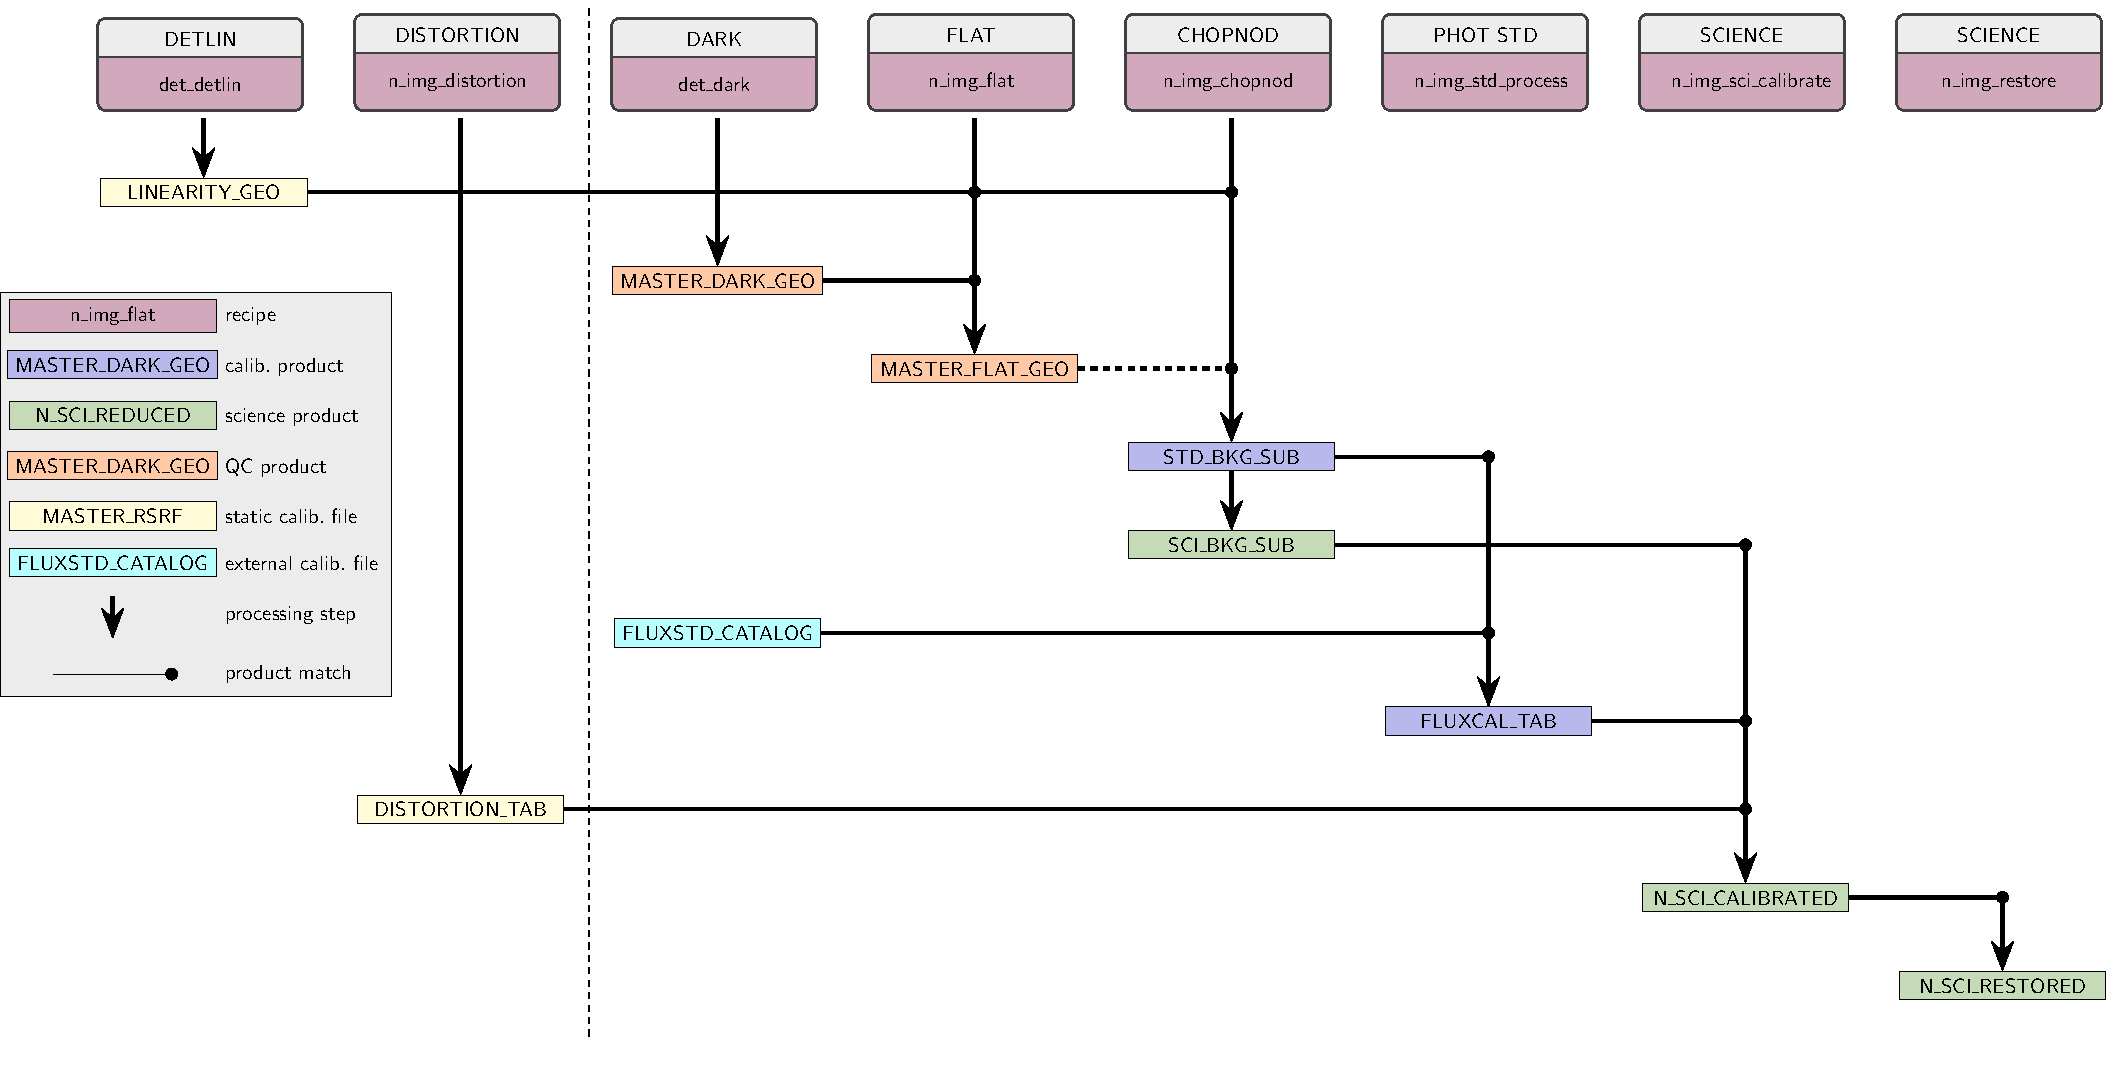
\includegraphics{IMG_N_assomap_tikz}
    \caption[Reduction cascade and association map for imaging in N]{%
      Association map for imaging in the N band. The figure shows
      only the primary product created from each recipe; for a full
      list of products refer to the recipe descriptions in
      Sect.~\ref{ssec:recipes_img_n}. The dashed line separates
      calibration tasks that are done at AIT or infrequently during
      operations (left) from daily tasks (right). The prefix ``\texttt{metis\_}'' has
      been omitted from the recipe names to improve clarity.}
    \label{fig:IMG_N_Assomap}
  \end{figure}
\end{landscape}

%%%%%%%%%%%%%%%%%%%%%%%%%%%%%%%%%%%%%%%%%%%%%%%%%%%%%%
%%% Local Variables:
%%% TeX-master: "METIS_DRLD"
%%% End:


%%%
\subsection{Long-Slit Spectroscopy in L/M- and N-bands}\label{lss:overview}
\subsubsection{The workflow cascades}\label{lss:cascade_overview}
The purpose of the pipeline is to correct or remove contributions from
the instrument, telescope, and atmosphere and generate science-grade
data products for the L/M- and N-band \ac{LSS}
mode. Since the detector properties are not fully specified, especially of the new Geosnap, we currently assume
basically the same reduction cascade for both spectral ranges LM and
N, respectively. The only major difference at the time being is the absence of \ac{WCU} laser sources in the N-band, which are only available during \ac{AIT} phase to generate a first guess of the pixel-to-wavelength relation. Therefore the first guess wavelength solution in the N-band will be based on that \ac{AIT} data. As we assume the instrument to be very stable, that approach should be sufficient for the low-resolution N-band spectroscopy. In the LM range, two fix-frequency lasers ($@3.39$µm and $@5.26$µm) and one tuneable ($4.68....4.78$µm) is foreseen in the \ac{WCU} to be taken on daily basis (cf. \cite{METIS-calibration_plan}). Although mainly foreseen to be used for the high-resolution spectroscopy \ac{LMS} mode, we can use these laser sources for the LM-band \ac{LSS} as well.

Special emphasis has to be drawn to the effects of the Earth's
atmosphere in several respects:
\begin{itemize}
\item Wavelength calibration: Absorption/emission features are intended to be
  used for the wavelength calibration. Thus, a good knowledge on /
  identification of these features is crucial for the accuracy of the
  wavelength calibration.
\item Telluric correction: In the MIR regime telluric absorption is
  one of the most dominant effects visible in spectra. Modelling
  approaches like \texttt{molecfit} heavily rely on accurate
  atmospheric input profiles, which represent the actual state and
  composition of the Earth's atmosphere. This especially applies to
  the \ac{PWV} content since this is the most
  dominant and most variable species.
\item Atmospheric dispersion: \ac{METIS} will have \ac{ADC}s compensating the
  effect of atmospheric dispersion. However, for technical reasons
  these ADCs are fixed at several positions. This means that the
  compensation is only partially. This leads to two practical effects:
  (a) wavelength-dependent slit losses, and (b) distortions in both,
  the spatial and the spectral direction (see \cite{METIS-ADC_study}
  for more details). For both, the pipeline needs to correct
  for. It is foreseen to determine these slitlosses on yearly basis with a separate calibration task (cf. \cite{METIS-calibration_plan}) and create a slit-loss table to be included in the static calibration database.
\end{itemize}

%However, to keep flexibility and independence of both branches, we
%define different recipes for the time being, although they will be
%mostly based on the same algorithms. We therefore focus here on the LM-band only.

Figures~\ref{Fig:LMLssAssomap1} and \ref{Fig:LMLssAssomap2} show the reduction cascade and the association map for the recipes handling L/M-long-slit
spectroscopy data.  Table~\ref{Tab:LMLssDatProc} contains the data processing table for this mode. For the N-band \ac{LSS} mode the cascade and the data processing table is given in Fig.\ref{Fig:NLssAssomap} and Table~\ref{Tab:NLssDatProc}, respectively (cf. also Fig.~\ref{Fig:LSScascadelegend}).

In general, there are four major steps in each of the two cascades:
\begin{itemize}
    \item \textbf{Preparation step:} This contains the recipes, which are invoked only rarely, e.g. after major instrument interventions, or on monthly/yearly basis to update the static calibration database. These recipes are therefore not shown in the cascade in Figs.~\ref{Fig:LMLssAssomap1}/\ref{Fig:LMLssAssomap2} and \ref{Fig:NLssAssomap} and the corresponding data processing tables. In case of the \ac{LSS} pipeline this concerns the creation of the gain maps/linearity checks (see Section~\ref{sssec:metis_det_lingain}), the determination of the slit losses induced by the fixed positions of the ADCs (cf. Section~\ref{sssec:adc_slitlosses} and Section "Calibration of slit losses" in Calibration plan \cite{METIS-calibration_plan}) and the zero position of the chopping mirror (see Section~\ref{ssec:metisimgchophome} and Section "Chopper Home Position" in \cite{METIS-calibration_plan} for more details). T
    \item \textbf{Basic steps}: The basic steps aim for correcting the detector influence, in particular the dark correction and the determination of the master \ac{RSRF}.
    \item \textbf{Calibration/correction steps}: This is the main part which incorporates the order trace detection, distortion, wavelength and flux correction.
    \item \textbf{Post-calibration steps}: After havig calibrated spectra at hand, the last step is the telluric absorption correction.
\end{itemize}

\begin{figure}[ht]
  \centering
  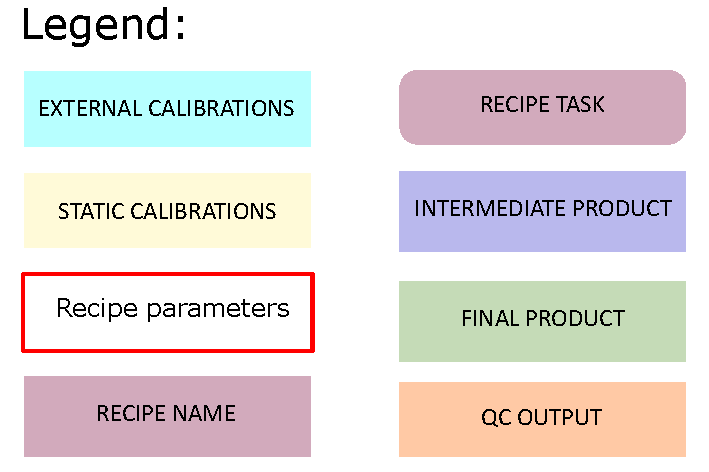
\includegraphics[width=0.4\textheight]{figures/legend.pdf}
  \caption[Legend]{Legend of the coloured boxes in the \ac{LSS} cascades.}
  \label{Fig:LSScascadelegend}
\end{figure}
\clearpage

\begin{sidewaysfigure}[ht]
  \centering
  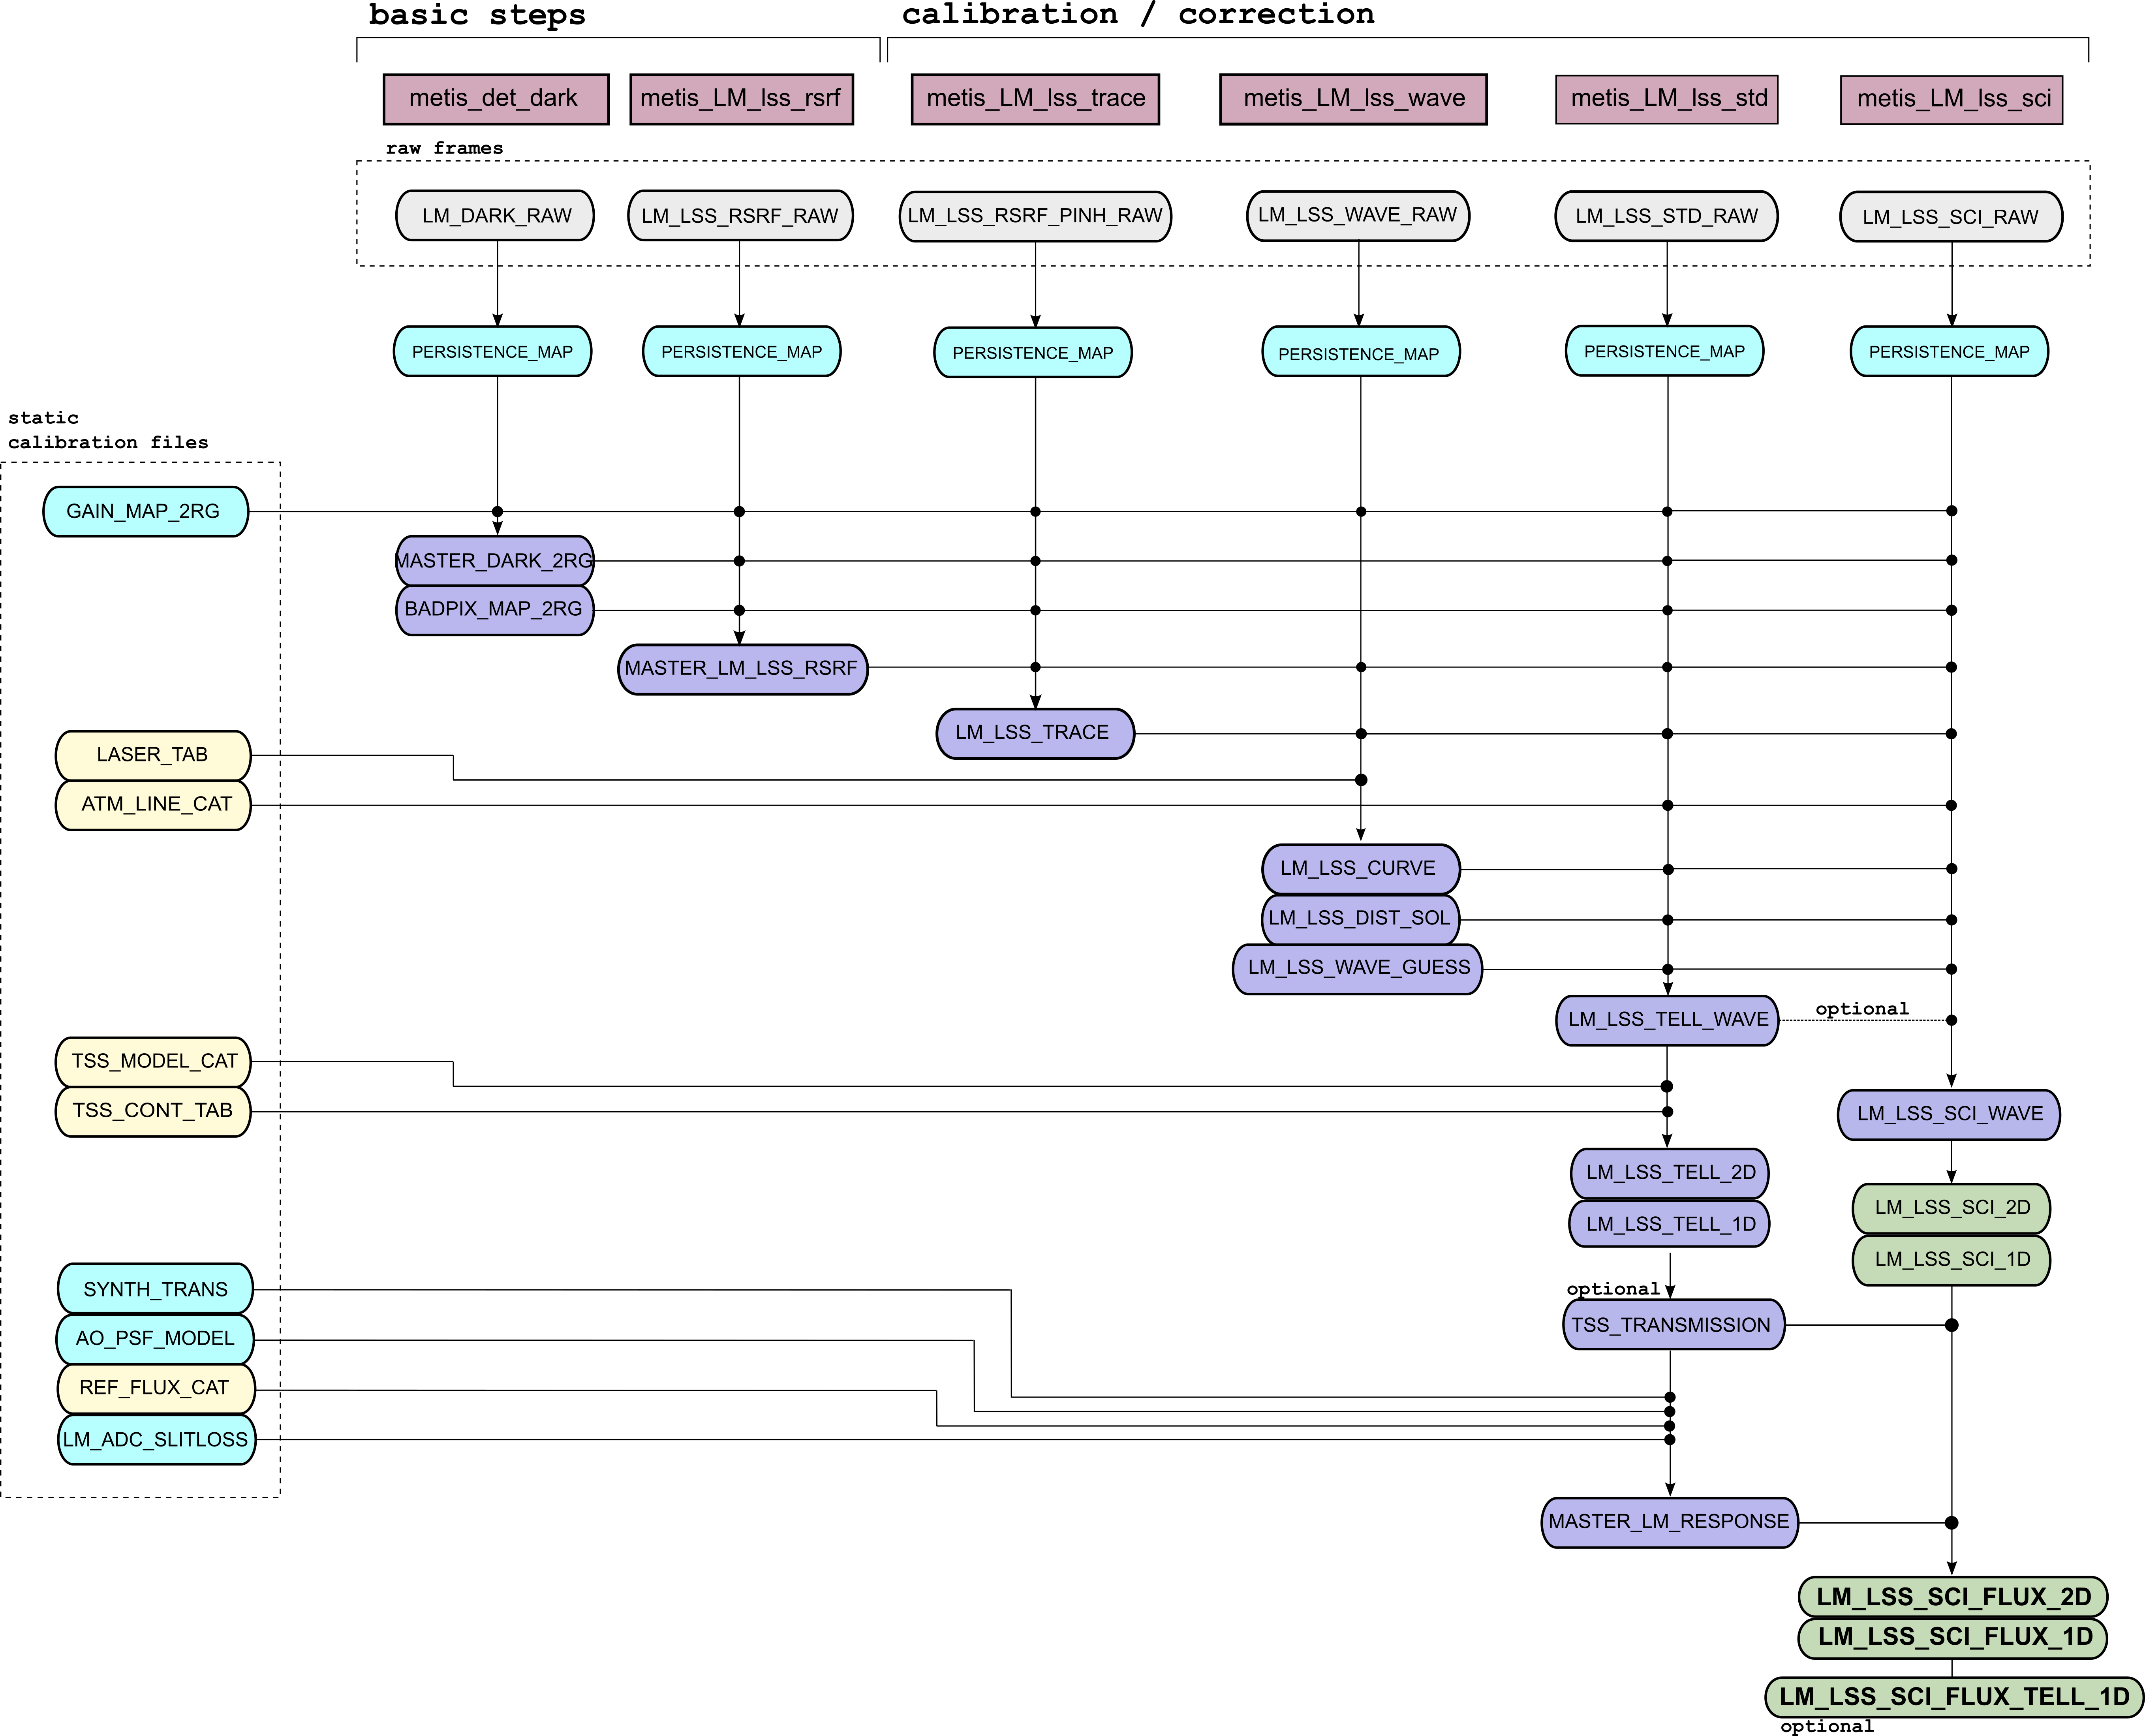
\includegraphics[width=0.9\textheight]{figures/LM_LSS_pipeline_wf_draft_latest_part_1_v0.80.png}
  \caption[Reduction cascade and association map for LM long-slit
  spectroscopy]{Part 1 of the reduction cascade and association map for long-slit
    spectroscopy in the LM bands.  }
  \label{Fig:LMLssAssomap1}
\end{sidewaysfigure}

\begin{sidewaysfigure}[ht]
  \centering
  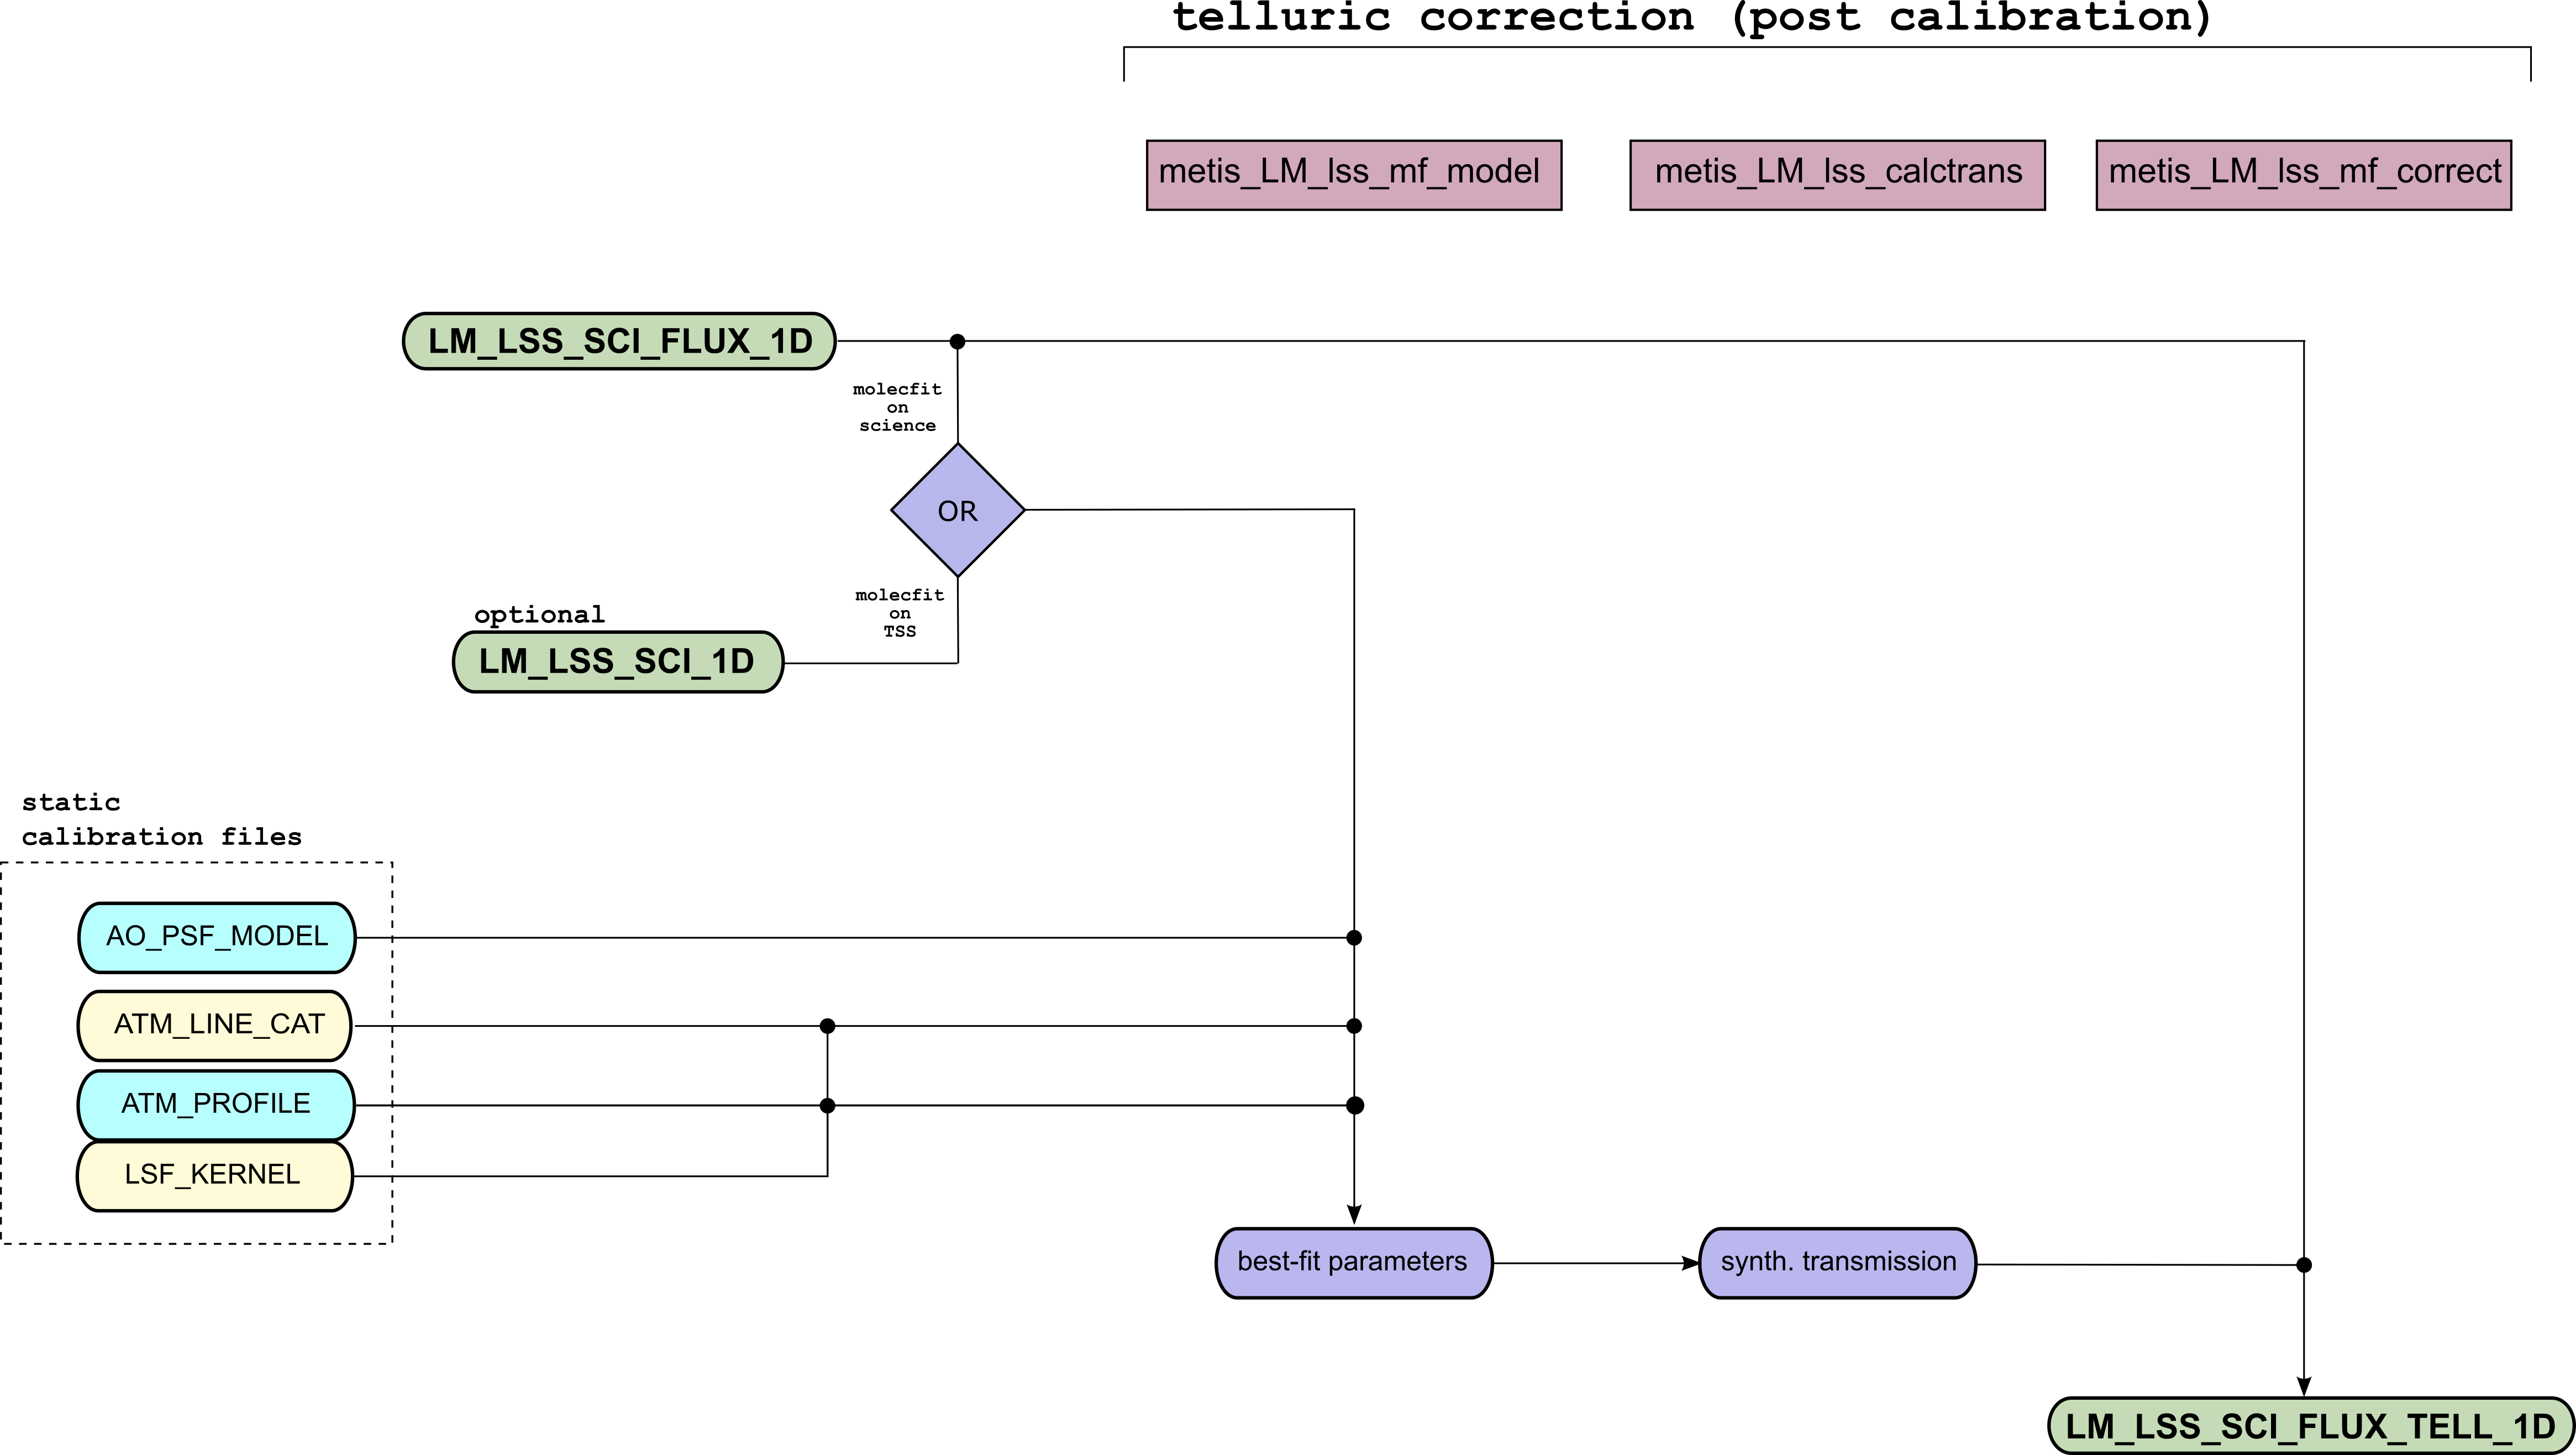
\includegraphics[width=0.8\textheight]{figures/LM_LSS_pipeline_wf_draft_latest_part_2_v0.80.png}
  \caption[Reduction cascade and association map for LM long-slit
  spectroscopy]{Part 2 of the reduction cascade and association map for long-slit
    spectroscopy in the LM bands.  }
  \label{Fig:LMLssAssomap2}
\end{sidewaysfigure}


% \begin{sidewaysfigure}[ht]
%   \centering
%   \includegraphics[width=0.9\textheight]{figures/NQ_LSS_pipeline_wf_draft_latest.png}
%   \caption[Reduction cascade and association map for N long-slit
%   spectroscopy]{Reduction cascade and association map for long-slit
%     spectroscopy in the N band.  }
%   \label{Fig:NQLssAssomap}
% \end{sidewaysfigure}


%% ---- Table: LM long-slit spectroscopy
\begin{sidewaystable}
  \footnotesize
  \begin{center}
    \caption[Data Processing table for LM long-slit spectroscopy]{%
      Data Processing table for LM long-slit spectroscopy
      calibration mode; }\bigskip
    \label{Tab:LMLssDatProc}
    \begin{tabular}{|l|l|l|l|l|l|}
      \hline
      Data Type   & Classification & Recipe (Level)	& FITS Keywords & static CalibDB & Products\\
    (Templates) & Keywords	 & Processing steps	&		&	  &	\\
    \hline
    \TPL{DARK}	& \CODE{DPR.CATG==CALIB} & \hyperref[sssec:metis_det_dark]{\REC{metis_det_dark}} & Exposure time	&	\hyperref[dataitem:gainmap2rg]{\PROD{GAIN_MAP_2RG}}& Averaged dark frame\\
    		& \CODE{DPR.TYPE==DARK}  &			&		&	& Bad pixel map\\
    		& \CODE{DPR.TECH==IMAGE}  &			&		&	& \\
    \hline
    \TPL{FLAT}	& \CODE{DPR.CATG==CALIB} & \hyperref[rec:lsslmrsrf]{\REC{metis_LM_lss_rsrf}} & Exposure time	& \hyperref[dataitem:gainmap2rg]{\PROD{GAIN_MAP_2RG}}	& Averaged, normalized flatfield\\
    		& \CODE{DPR.TYPE==FLAT}  &			&	Grism	& 	& \\
    		& \CODE{DPR.TECH==SPECTRUM}  &			&	Slit	&	& \\
    \hline
         	& \CODE{DPR.CATG==CALIB} &\hyperref[rec:lsslmtrace]{\REC{metis_LM_lss_trace}} & Exposure time	& \hyperref[dataitem:gainmap2rg]{\PROD{GAIN_MAP_2RG}}	& Order location\\
    		& \CODE{DPR.TYPE==FLAT}  &			&		&	& (polynomial fit)\\
    		& \CODE{DPR.TECH==SPECTRUM}  &			&		&	& \\
    \hline
    \TPL{WAVE,LASER} & \CODE{DPR.CATG==CATG} &\hyperref[rec:lsslmwave]{\REC{metis_LM_lss_wave}} & Exposure time &  \hyperref[dataitem:gainmap2rg]{\PROD{GAIN_MAP_2RG}} & wavelength solution\\
    		& \CODE{DPR.TYPE==WAVE,LASER}   &			   & Grism & \hyperref[dataitem:lasertab]{\STATCALIB{LASER_TAB}} &\\
    		& \CODE{DPR.TECH==SPECTRUM}  &			& Slit		&	& \\
    		& \CODE{PRO.CATG==SPECTRUM}   &  &  & & \\
    \hline
    \TPL{FLUX,STD} & \CODE{DPR.CATG==CALIB} & \hyperref[rec:lsslmstd]{\REC{metis_LM_lss_flux}}& Object name (Flux STD) & \hyperref[dataitem:gainmap2rg]{\PROD{GAIN_MAP_2RG}} & Instrumental\\
    		& \CODE{DPR.TYPE==FLUX,STD}   &			   & Exposure time & \hyperref[dataitem:atmlinecat]{\EXTCALIB{ATM_LINE_CAT}} & response function\\
    		& \CODE{DPR.TECH==SPECTRUM}  &			&	Grism	&	\hyperref[dataitem:lmsynthtrans]{\STATCALIB{LM_SYNTH_TRANS}}& \\
    		& \CODE{PRO.CATG==SPECTRUM}   &  & Slit & \hyperref[dataitem:lmadcslitloss]{\STATCALIB{LM_ADC_SLITLOSS}} & \\
    		& & & & \hyperref[dataitem:aopsfmodel]{\EXTCALIB{AO_PSF_MODEL}} &\\    
    		& & & & \hyperref[dataitem:reffluxcat]{\STATCALIB{REF_FLUX_CAT}} &\\    \hline
    \TPL{SCIENCE} & \CODE{DPR.CATG==SCIENCE} & \hyperref[rec:lsslmsci]{\REC{metis_LM_lss_sci}} & Object name &  \hyperref[dataitem:gainmap2rg]{\PROD{GAIN_MAP_2RG}} & Science grade spectrum\\
    		& \CODE{DPR.TYPE==OBJECT}   &			   & Exposure time & \hyperref[dataitem:lmadcslitloss]{\STATCALIB{LM_ADC_SLITLOSS}} &\\
    		& \CODE{DPR.TECH==SPECTRUM}  &			&	Grism	& \hyperref[dataitem:atmlinecat]{\EXTCALIB{ATM_LINE_CAT}}	& \\
    		& \CODE{PRO.CATG==SPECTRUM}   &  & Slit  &  & \\
    \hline
            & \CODE{DPR.CATG==SCIENCE} & \hyperref[rec:LMLSSmfmodel]{\REC{metis_LM_lss_mf_model}} & Object name & \hyperref[dataitem:lsfkernel]{\STATCALIB{LSF_KERNEL}}	 & Best-fit \\
    		& \CODE{DPR.TYPE==OBJECT}   &			  & & \hyperref[dataitem:atmprofile]{\EXTCALIB{ATM_PROFILE}}  & \texttt{molecfit} parameters\\
    		& \CODE{DPR.TECH==TBD}  &			&		& \hyperref[dataitem:atmlinecat]{\EXTCALIB{ATM_LINE_CAT}}	& \\
    		& \CODE{PRO.CATG==TBD}   &  &  & start parameter set & \\
    \hline
            & \CODE{DPR.CATG==SCIENCE} &  \hyperref[rec:LMLSSmfcalctrans]{\REC{metis_LM_lss_mf_calctrans}} & Object name & \hyperref[dataitem:atmlinecat]{\EXTCALIB{ATM_LINE_CAT}}	 & synthetic \\
    		& \CODE{DPR.TYPE==LSS}   &		&	   &   & Transmission curve\\
    		& \CODE{DPR.TECH==TBD}  &			&		& 	& \\
    		& \CODE{PRO.CATG==TBD}   &  &  & & \\
    \hline
            & \CODE{DPR.CATG==SCIENCE} &  \hyperref[rec:LMLSSmfcorrect]{\REC{metis_LM_lss_mf_correct}} & Object name & 	 & Absorption corrected\\
    		& \CODE{DPR.TYPE==LSS}   &			   & & synthetic Transmission curve  & science spectrum\\
    		& \CODE{DPR.TECH==TBD}  &			&		&	& \\
    		& \CODE{PRO.CATG==TBD}   &  &  & & \\
    \hline
    \end{tabular}
  \end{center}
\end{sidewaystable}

\begin{sidewaysfigure}[ht]
  \centering
  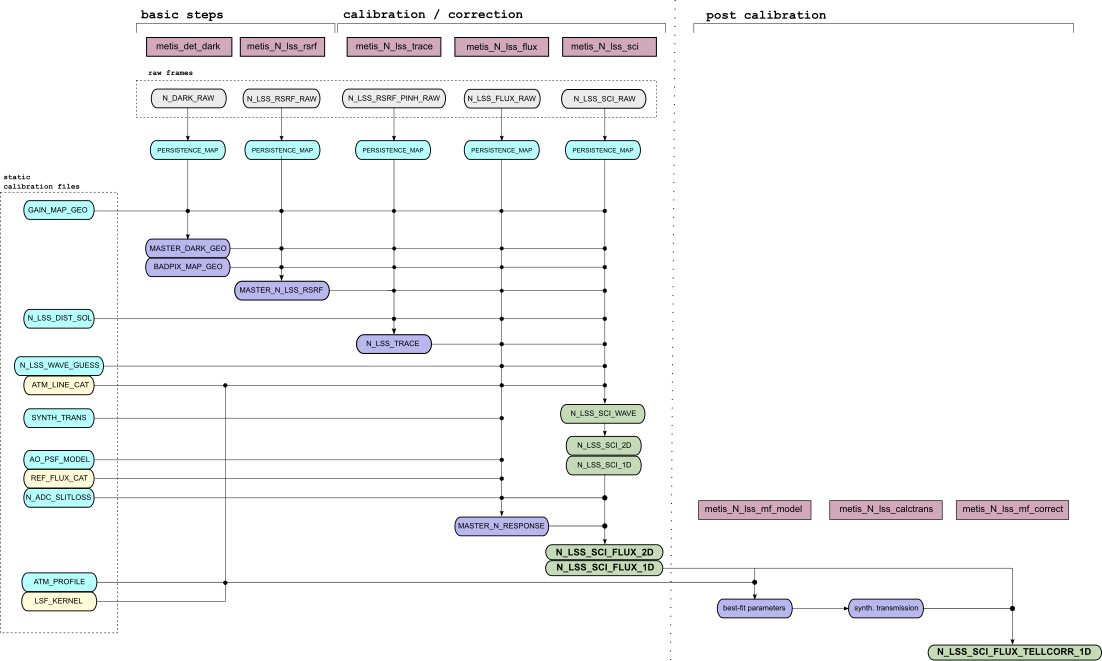
\includegraphics[width=0.9\textheight]{figures/N_LSS_pipeline_wf_draft_latest_v0.74.png}
  \caption[Reduction cascade and association map for N long-slit
  spectroscopy]{Reduction cascade and association map for long-slit
    spectroscopy in the N bands. }
  \label{Fig:NLssAssomap}
\end{sidewaysfigure}

%% ---- Table: N long-slit spectroscopy
\begin{sidewaystable}
  \footnotesize
  \begin{center}
    \caption[Data Processing table for N-band long-slit spectroscopy]{%
      Data Processing table for N long-slit spectroscopy
      calibration mode}\bigskip
    \label{Tab:NLssDatProc}
    \begin{tabular}{|l|l|l|l|l|l|}
      \hline
      Data Type   & Classification & Recipe (Level)	& FITS Keywords & static CalibDB & Products\\
    (Templates) & Keywords	 & Processing steps	&		&	  &	\\
    \hline
    \TPL{DARK}	& \CODE{DPR.CATG==CALIB} & \hyperref[sssec:metis_det_dark]{\REC{metis_det_dark}} & Exposure time	& \hyperref[dataitem:gainmap2rg]{\PROD{GAIN_MAP_GEO}}	& Averaged dark frame\\
    		& \CODE{DPR.TYPE==DARK}  &			&		&	& Bad pixel map\\
    		& \CODE{DPR.TECH==IMAGE}  &			&		&	& \\
    \hline
    \TPL{FLAT}	& \CODE{DPR.CATG==CALIB} & \hyperref[rec:lssnrsrf]{\REC{metis_N_lss_rsrf}} & Exposure time	& \hyperref[dataitem:gainmap2rg]{\PROD{GAIN_MAP_GEO}}	& Averaged, normalized flatfield (\ac{RSRF}\\
    		& \CODE{DPR.TYPE==FLAT}  &			&	Grism	&	& Bad pixel map\\
    		& \CODE{DPR.TECH==SPECTRUM}  &			& Slit		&	& \\
    \hline
         	& \CODE{DPR.CATG==CALIB} & \hyperref[rec:lssntrace]{\REC{metis_N_lss_trace} }& Exposure time	& \hyperref[dataitem:gainmap2rg]{\PROD{GAIN_MAP_GEO}}	& Order location\\
    		& \CODE{DPR.TYPE==FLAT}  &			&	Grism	&	& (polynomial fit)\\
    		& \CODE{DPR.TECH==SPECTRUM}  &			&	Slit	&	& \\
    \hline
    \TPL{FLUX,STD} & \CODE{DPR.CATG==CALIB} & \hyperref[rec:lssnflux]{\REC{metis_N_lss_flux}} & Object name (Flux STD) & \hyperref[dataitem:gainmap2rg]{\PROD{GAIN_MAP_GEO}} & Instrumental\\
    		& \CODE{DPR.TYPE==FLUX,STD}   &			   & Exposure time & \hyperref[dataitem:nlsswaveguess]{\STATCALIB{N_LSS_WAVE_GUESS}} & response function\\
    		& \CODE{DPR.TECH==SPECTRUM}   &			   & Grism		& \hyperref[dataitem:atmlinecat]{\EXTCALIB{ATM_LINE_CAT}}	& \\
    		& \CODE{PRO.CATG==SPECTRUM}   &  &  Slit & \hyperref[dataitem:nsynthtrans]{\STATCALIB{N_SYNTH_TRANS}} & \\
    		& & & & \hyperref[dataitem:nadcslitloss]{\STATCALIB{N_ADC_SLITLOSS}} &\\
    		& & & &  \hyperref[dataitem:reffluxcat]{\STATCALIB{REF_FLUX_CAT}} &\\
    		& & & & \hyperref[dataitem:aopsfmodel]{\EXTCALIB{AO_PSF_MODEL}} &\\
    		& & & & \hyperref[dataitem:nlssdistsol]{\STATCALIB{N_LSS_DIST_SOL}} &\\
    		& & & & \hyperref[dataitem:reffluxcat]{\STATCALIB{REF_FLUX_CAT}} &\\
    \hline
    \TPL{SCIENCE} & \CODE{DPR.CATG==SCIENCE} & \hyperref[rec:lssnsci]{\REC{metis_N_lss_sci}} & Object name & \hyperref[dataitem:gainmap2rg]{\PROD{GAIN_MAP_GEO}}  & Science grade spectrum\\
    		& \CODE{DPR.TYPE==OBJECT}   &			   & Exposure time &  \hyperref[dataitem:atmlinecat]{\EXTCALIB{ATM_LINE_CAT}} &\\
    		& \CODE{DPR.TECH==SPECTRUM}  &			&	Grism	&\hyperref[dataitem:nadcslitloss]{\STATCALIB{N_ADC_SLITLOSS}}	& \\
    		& \CODE{PRO.CATG==SPECTRUM}   &  & Slit & \hyperref[dataitem:nlsswaveguess]{\STATCALIB{N_LSS_WAVE_GUESS}} & \\
    		& & & & \hyperref[dataitem:nlssdistsol]{\STATCALIB{N_LSS_DIST_SOL}} &\\
    \hline
            & \CODE{DPR.CATG==SCIENCE} & \hyperref[rec:NLSSmfmodel]{\REC{metis_N_lss_mf_model}} & Object name & \hyperref[dataitem:lsfkernel]{\STATCALIB{LSF_KERNEL}}	 & Best-fit \\
    		& \CODE{DPR.TYPE==OBJECT}   &			  & & \hyperref[dataitem:atmprofile]{\EXTCALIB{ATM_PROFILE}}  & \texttt{molecfit} parameters\\
    		& \CODE{DPR.TECH==TBD}  &			&		& \hyperref[dataitem:atmlinecat]{\EXTCALIB{ATM_LINE_CAT}}	& \\
    		& \CODE{PRO.CATG==TBD}   &  &  & start parameter set & \\
    \hline
            & \CODE{DPR.CATG==SCIENCE} & \hyperref[rec:NLSSmfcalctrans]{\REC{metis_N_lss_mf_calctrans}} & Object name & \hyperref[dataitem:atmlinecat]{\EXTCALIB{ATM_LINE_CAT}}	 & synthetic \\
    		& \CODE{DPR.TYPE==LSS}   &		&	   &  & Transmission curve\\
    		& \CODE{DPR.TECH==TBD}  &			&		&  	& \\
    		& \CODE{PRO.CATG==TBD}   &  &  & & \\
    \hline
            & \CODE{DPR.CATG==SCIENCE} & \hyperref[rec:NLSSmfcorrect]{\REC{metis_N_lss_mf_correct}} & Object name & 	 & Absorption corrected\\
    		& \CODE{DPR.TYPE==LSS}   &			   &  & synthetic Transmission curve & science spectrum\\
    		& \CODE{DPR.TECH==TBD}  &			&		&	& \\
    		& \CODE{PRO.CATG==TBD}   &  &  & & \\
    \hline
    \end{tabular}
  \end{center}
\end{sidewaystable}

\subsubsection{Static calibration database}\label{lss:static_calib}
The static calibration database comprises several data sets, some are updated from time to time:
\begin{itemize}
    \item \hyperref[dataitem:gainmap2rg]{\hyperref[dataitem:gainmap2rg]{\PROD{GAIN_MAP_2RG}}} and \hyperref[dataitem:gainmapgeo]{\hyperref[dataitem:gainmap2rg]{\PROD{GAIN_MAP_GEO}}}: These are the detector gain maps of the detectors (2RG=Hawaii2RG, LM-band; GEO=Geosnap, N-band), which are created by the recipe \hyperref[sssec:metis_det_lingain]{\REC{metis_det_lingain}} (see Section~\ref{sssec:metis_det_lingain}). This recipe also checks the linearity of the pixels and is carried out every once in a while (yearly, TBD, see \cite{METIS-calibration_plan}) as we assume the detectors to be fairly stable.
    \item \hyperref[dataitem:lasertab]{\STATCALIB{LASER_TAB}}: The \ac{WCU} provides laser sources for the first guess of the wavelength solution. The main laser frequencies are fixed (\cite{METIS-calibration_plan}) and given in a static table.
    \item \hyperref[dataitem:atmlinecat]{\EXTCALIB{ATM_LINE_CAT}}: The main wavelength calibration will be done by means of atmospheric lines, most probably based on the \ac{HITRAN}\footnote{\url{https://hitran.org/}}. They are given in a static catalogue. This database is also required by the telluric correction package \texttt{molecfit}.
    \item \hyperref[dataitem:lmsynthtrans]{\STATCALIB{LM_SYNTH_TRANS}}/\hyperref[dataitem:nsynthtrans]{\STATCALIB{N_SYNTH_TRANS}}: For the determination of the continuum of flux standard stars a rough telluric correction is needed. We intend to apply static transmission curves for that purpose as we deem it to be sufficient and more time efficient than applying the telluric correction package \texttt{molecfit} every time. This static transmission curve will be determined during commissioning via \texttt{molecfit}.
    \item \hyperref[dataitem:aopsfmodel]{\EXTCALIB{AO_PSF_MODEL}}: For the determination of \ac{AO}-induced slit losses we intend to use a static \ac{PSF} model, which is scaled by the \ac{AO} telemetry data. Details on that are TBD.
    \item \hyperref[dataitem:reffluxcat]{\STATCALIB{REF_FLUX_CAT}}: The absolute flux calibration will be done by observations of specific flux standard stars, which are compared to their theoretical models. The \hyperref[dataitem:reffluxcat]{\STATCALIB{REF_FLUX_CAT}} will contain these models. Currently, the catalogue of flux standard stars comprises the stars from the catalogue of the \ac{VISIR} instrument.

    \item \hyperref[dataitem:tssmodelcat]{\STATCALIB{TSS_MODEL_CAT}}: In some cases, the default modelling method for the telluric correction might not be possible or leading to bad results. We therefore foresee the possibility to use telluric standard stars. For the determination of the transmisison function a model of the selected telluric star is required. In this table, a model of a set of such stars
    \item \hyperref[dataitem:tssconttab]{\STATCALIB{TSS_CONT_TAB}}: 

    \item \hyperref[dataitem:lmadcslitloss]{\STATCALIB{LM_ADC_SLITLOSS}}/\hyperref[dataitem:nadcslitloss]{\STATCALIB{N_ADC_SLITLOSS}}: It is expected that the fixed positions of the \ac{ADC} will introduce specific slit losses. These losses are determined in the recipes \hyperref[rec:metislmadcmslitloss]{\REC{metis_lm_adc_slitloss}} and \hyperref[rec:metisnadcmslitloss]{\REC{metis_n_adc_slitloss}} (see Section~\ref{sssec:adc_slitlosses} and \cite{METIS-calibration_plan}). As these losses are assumed to be very stable, these recipes will be carried out only rarely.
    \item \hyperref[dataitem:atmprofile]{\EXTCALIB{ATM_PROFILE}} and \hyperref[dataitem:lsfkernel]{\STATCALIB{LSF_KERNEL}}: The telluric correction package \texttt{molecfit} requires an atmospheric profile incorporating height information of the temperature, pressure and molecular abundances as input. Currently we use a static profile (equatorial \texttt{equ.atm}\footnote{\url{https://eodg.atm.ox.ac.uk/RFM/atm/}}) as starting point of the fit of the molecular column densities. In addition, a kernel for the \ac{LSF} is provided. We intend to determine the kernel during commissioning and use this as input. However, it is still unclear in how far the \ac{AO} influences that kernel. The current baseline is to use the static \hyperref[dataitem:lsfkernel]{\STATCALIB{LSF_KERNEL}} as starting point for fitting the line spread function.
    \item \hyperref[dataitem:nlssdistsol]{\STATCALIB{N_LSS_DIST_SOL}}/\hyperref[dataitem:nlsswaveguess]{\STATCALIB{N_LSS_WAVE_GUESS}}: First guess solutions of the N-band LSS mode are static due to the absence of laser sources after \ac{AIT}. As the instrument is expected to be very stable, these calibration files will be created only once and kept static.
\end{itemize}

%%%
\subsection{LM IFU: integral-field spectroscopy}
\label{ssec:overview_ifu}

The \ac{IFU} pipeline has not yet been revised since PDR, hence the
description in \cite{DRLS} applies. For reference, the association map
is shown in Fig.~\ref{Fig:IfuAssomap}.

We will consider rearranging the recipes to be in line with the
imaging pipelines. This would entail handling basic reduction and
background subtraction for of both science and standard exposures in
common recipes (\REC{metis_ifu_basic}, \REC{metis_ifu_background}),
then having a recipe to analyse the standard observations
(\REC{metis_ifu_photstd}). The science exposures are then fully
calibrated (\REC{metis_ifu_calibrate}). A full set of exposures would
then be assembled and restored with a fully sampled PSF in a
post-processing recipe (\REC{metis_ifu_combine}).

\begin{sidewaysfigure}[ht]
  \centering
  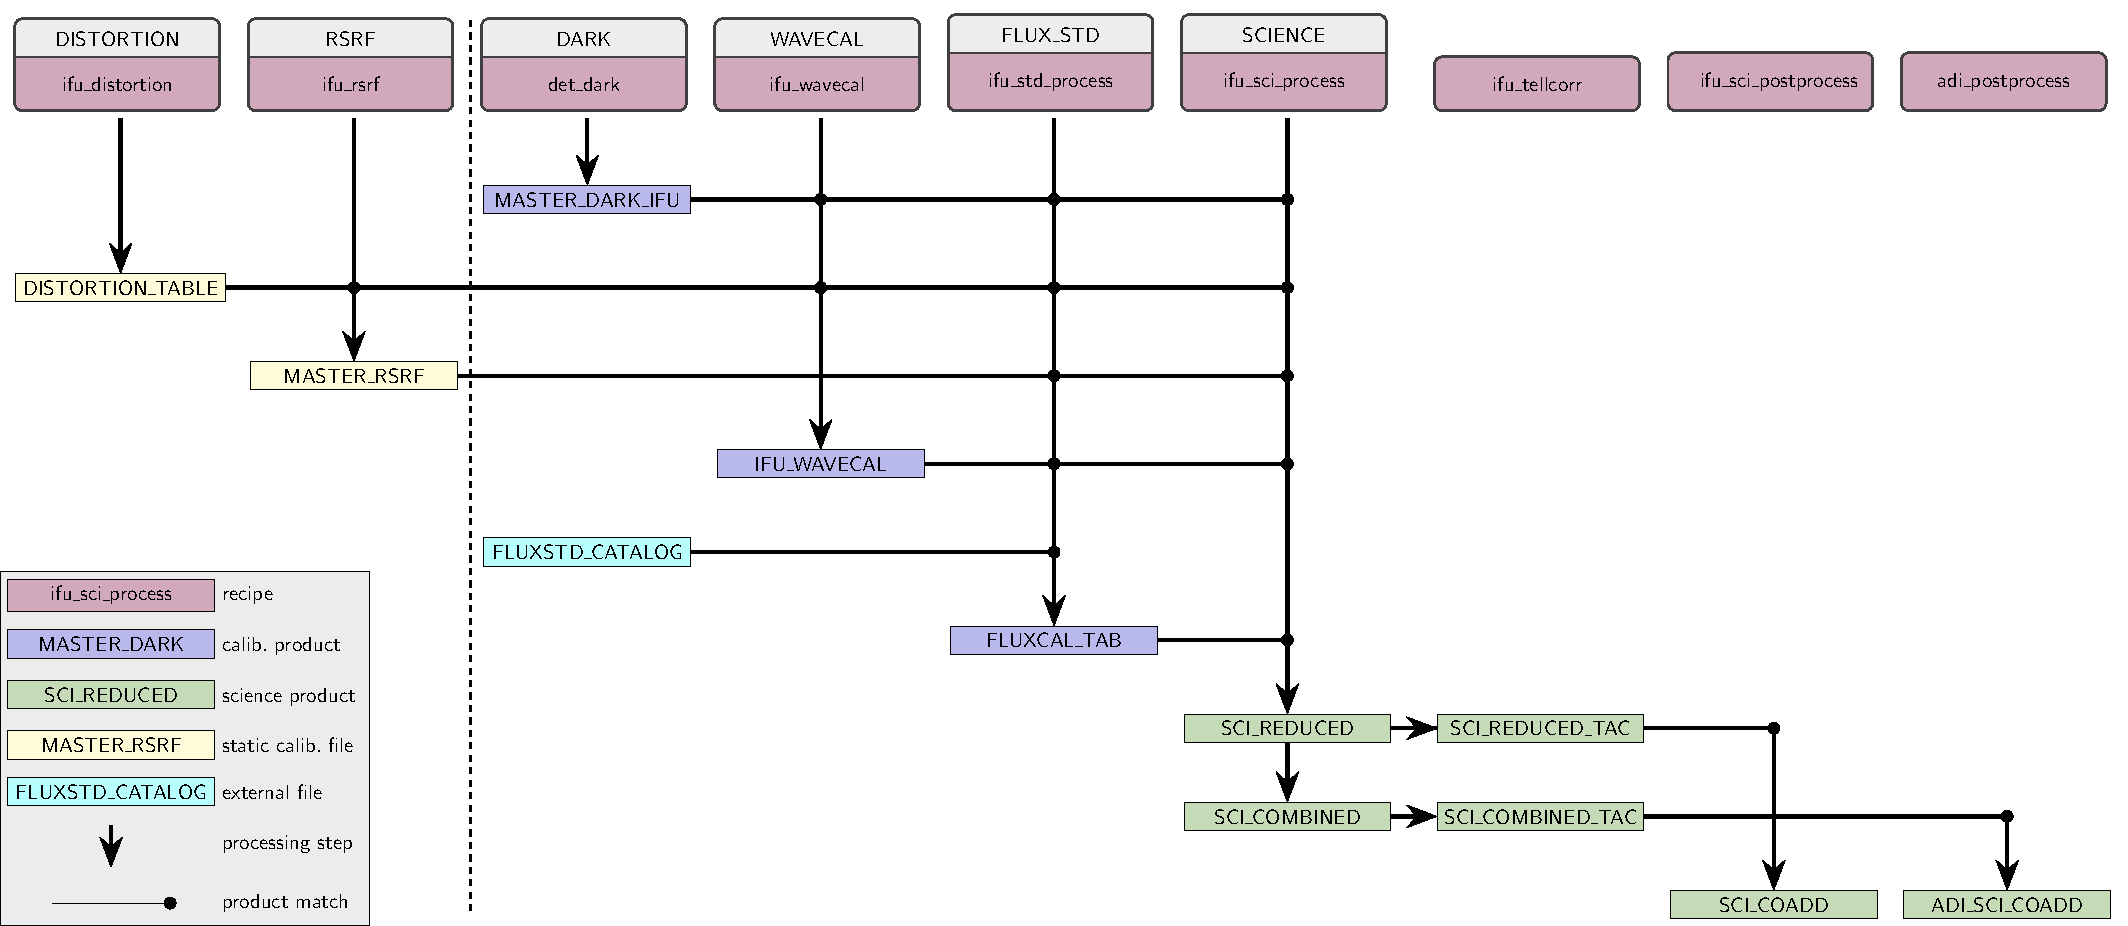
\includegraphics[width=\textheight]{IFU_assomap_tikz}
  \caption[Reduction cascade and association map for IFU
  spectroscopy]{%
    Association map for \ac{IFU} spectroscopy in L- and M-band. The
    figure shows only the primary products created by each recipe; for
    a full list of products refer to the recipe descriptions in
    Sect.~\ref{ssec:IFU_recipes}. The dashed line separates
    calibration tasks that are done at AIT or infrequently during
    operations from tasks done daily. The prefix ``\REC{metis_}'' has been
    omitted from the recipe names to improve clarity.}
  \label{Fig:IfuAssomap}
\end{sidewaysfigure}



%%%%%%%%%%%%%%%%%%%%%%%%%%%%%%%%%%%%%%%%%%%%%%%%%%%%%%

%%% Local Variables:
%%% TeX-master: "METIS_DRLD"
%%% End:


\subsection{Parallel Observing Modes}
\label{ssec:combinedmodes}

There are three parallel observing modes:

\begin{itemize}
\item Parallel observing mode IMG-LM and IMG-N (Section~\ref{sssec:parallellmnimg})
\item Parallel observing mode LSS-LM and LSS-N (Section~\ref{sssec:parallellmnspec})
\item Parallel observing mode IMG-LM and IFU (Section~\ref{sssec:parallellmnspec})
\end{itemize}

The respective templates corresponding to these modes will produce raw data files that can be processed independently by the relevant workflows.
That is, the templates will trigger two different recipe cascades, and there are no specific recipes for any of the parallel observing modes.

\subsubsection{Parallel observing mode IMG-LM and IMG-N}\label{sssec:parallellmnimg}
There are two specific templates for parallel imaging observations in the LM-band and N-band:
\begin{itemize}
 \item \TPL{METIS_img_lmn_obs_AutoChopNod}
 \item \TPL{METIS_img_lmn_obs_GenericChopNod}
\end{itemize}
These templates produce two kind of raw images that are processed independently in either the LM-band or N-band imaging workflow.
This fulfills \REQ{METIS-7244}.


\subsubsection{Parallel observing mode LSS-LM and LSS-N}\label{sssec:parallellmnspec}
There is one specific template for parallel LSS observations in the LM-band and N-band:
\begin{itemize}
 \item \TPL{METIS_spec_lmn_obs_AutoChopNodOnSlit}
\end{itemize}
These templates produce two kind of raw images that are processed independently in either the LM-band or N-band LSS workflow.
This fulfills \REQ{METIS-7245}.

\subsubsection{Parallel observing mode IMG-LM and IFU}\label{sssec:parallellmifu}
Parallel observing mode IMG-LM and IFU is also needed to perform non-common path pointing and aberration correction in \ac{HCI} modes:
real-time monitoring of non-common path aberrations between the \ac{SCAO} \ac{WFS} and the \ac{HCI} elements cannot be performed with the \ac{IFU} due to slicing and sampling issues.

The IFU pickoff optic is a beamsplitter with a transmission of ~10\% to the LM imager and a reflectivity of ~90\% to the IFU. % https://polarion.astron.nl/polarion/#/project/METIS/workitem?id=METIS-3111
LM-band images can therefore be taken in parallel with the IFU exposures, for any of the IFU templates.
The LM-band images and IFU exposures are processed independently.
This fulfills \REQ{METIS-6072}.


\subsection{Workflows}
The association matrices described in the previous sections will be converted one-to-one into Reflex or \ac{EDPS} workflows.

Any interactivity in the workflows is described with the individual recipes.


\subsection{Matched FITS keywords}

The workflow management system (e.g. \ac{EDPS}) uses the `matched keywords'
to find calibration data when processing data.
That is, the system will compare the FITS keywords of the primary input, to
the FITS headers of the pool of possible calibration files to use, in order
to decide what data to use.

For example, most calibration data has to be taken with the same \FITS{DET.DIT}
and \FITS{DET.NDIT} combination as the science data.
Several calibration products also need to use the same filter, or the same mask, or the same grism as the science data.

All selections are done on equality.
That is, no interpolation between, e.g., \FITS{DET.DIT}, will be done if only an approximate matching data product is found.

The following two tables provide an overview of the matched FITS
keywords. Table~\ref{tab:fitskeywordaliasses} defines several high level keyword
aliases used for convenience when there are several combinations
of instrumental keywords (INS.) which are needed to match with the correct
calibration files. These keywords are used in the Matched Keyword
descriptions in the recipes in Chapter~\ref{sec:pipeline_recipes}.
Table~\ref{tab:fitsmatchedkeywordssummary}
summaries the input data, calibration files, and the FITS
keyworlds needed to match them for all the recipes listed in
Chapter~\ref{sec:pipeline_recipes}. The second defines various high
level aliases used for convenience when there are several combinations
of instrumental keywords which are needed to match with the correct
calibration files.

\begin{table}
    \caption{FITS keyword aliases}
    \label{tab:fitskeywordaliasses}
  \begin{tabular}[c]{|p{3cm}|p{5cm}|p{5cm}|}
      \hline
      \textbf{Alias} & \textbf{Description} & \textbf{FITS keywords} \\
      \hline
\FITS{DRS.FILTER}   & Filter Information (LM or N)  & value of \FITS{INS.OPTI10.NAME} or \FITS{INS.OPTI13.NAME} \\
\FITS{DRS.NDFILTER} & ND Filter information	        & value of \FITS{INS.OPTI11.NAME} or \FITS{INS.OPTI13.NAME} \\
\FITS{DRS.SLIT}     & Slit Information (LM or N)    & value of \FITS{INS.OPTI3.NAME} and \FITS{INS.OPTI12.NAME} or  \FITS{INS.OPTI9.NAME} \\
\FITS{DRS.MASK}     & Mask information for Coronagraphy	& value of \FITS{INS.OPTI1.NAME}, \FITS{INS.OPTI3.NAME}, \FITS{INS.OPTI5.NAME}, \FITS{INS.OPTI9.NAME}, \FITS{INS.OPTI12.NAME} \\
\FITS{DRS.PUPIL}    & Pupil information             & value of \FITS{INS.OPTI15.NAME} or \FITS{INS.OPTI16.NAME}\\
\hline
    \end{tabular}
\end{table}


\newgeometry{bottom=0.1cm, right=0.1cm, left=0.1cm, top=0.1cm}
\begin{landscape}
{
  \begin{longtable}[c]{|p{4.2cm}|p{4.6cm}|p{5.6cm}|p{3.5cm}|p{3.5cm}|}
%  \begin{longtable}[c]{|l|l|l|l|l|}
 \caption{FITS matched keywords summary}
 \label{tab:fitsmatchedkeywordssummary}
 \endfirsthead
 \hline
 \textbf{Recipe} & \textbf{Main Input} & \textbf{Calibration Data} & \textbf{FITS keywords} & \textbf{Aliases} \\
 \hline
    \endhead
 \hline
 \textbf{Recipe} & \textbf{Main Input} & \textbf{Calibration Data} & \textbf{FITS keywords} & \textbf{Aliases} \\
 \hline
\REC{metis_det_lingain} & \RAW{DETLIN_det_RAW}, \RAW{det_WCU_OFF_RAW} &  &  &  \\
\REC{metis_det_dark} & \RAW{DARK_det_RAW} & \PROD{LINEARITY_det}, \PROD{PERSISTENCE_MAP} &  &  \\
\REC{metis_det_persistence} &  &  &  &  \\
\REC{metis_lm_img_flat} & \RAW{LM_FLAT_LAMP_RAW}, \RAW{LM_FLAT_TWILIGHT_RAW} & \PROD{MASTER_DARK_2RG} & \FITS{DET.DIT}, \FITS{DET.NDIT}, \FITS{INS.OPTI10.NAME} & \FITS{DET.DIT}, \FITS{DET.NDIT}, \FITS{DRS.FILTER},  \\
\REC{metis_lm_img_basic_reduce} & \RAW{LM_IMAGE_SCI_RAW} & \PROD{MASTER_DARK_2RG}, \PROD{MASTER_IMG_FLAT_LAMP_LM}, \PROD{MASTER_IMG_FLAT_TWILIGHT_LM} & \FITS{DET.DIT}, \FITS{DET.NDIT}, \FITS{INS.OPTI10.NAME} & \FITS{DET.DIT}, \FITS{DET.NDIT}, \FITS{DRS.FILTER},  \\
\REC{metis_lm_img_background} & \RAW{LM_SCI_BASIC_REDUCED}, \RAW{LM_STD_BASIC_REDUCED} &  & \FITS{INS.OPTI10.NAME} & \FITS{DRS.FILTER},  \\
\REC{metis_lm_img_std_process} & \RAW{LM_STD_BKG_SUBTRACTED} & \PROD{FLUXSTD_CATALOG} & \FITS{INS.OPTI10.NAME} & \FITS{DRS.FILTER},  \\
\REC{metis_lm_img_calibrate} & \RAW{LM_SCI_BKG_SUBTRACTED} & \PROD{FLUXCAL_TAB}, \PROD{LM_DISTORTION_TABLE} & \FITS{INS.OPTI10.NAME} & \FITS{DRS.FILTER},  \\
\REC{metis_lm_img_sci_postprocess} & \RAW{LM_SCI_CALIBRATED} &  & \FITS{INS.OPTI10.NAME} & \FITS{DRS.FILTER},  \\
\REC{metis_lm_img_distortion} & \RAW{LM_DISTORTION_RAW}, \RAW{LM_WCU_OFF_RAW} & \EXTCALIB{PINHOLE_TABLE} & \FITS{INS.OPTI10.NAME} & \FITS{DRS.FILTER},  \\
\REC{metis_n_img_flat} & \RAW{N_FLAT_LAMP_RAW}, \RAW{N_FLAT_TWILIGHT_RAW} & \PROD{MASTER_DARK_GEO} & \FITS{DET.DIT}, \FITS{DET.NDIT}, \FITS{INS.OPTI10.NAME} & \FITS{DET.DIT}, \FITS{DET.NDIT}, \FITS{DRS.FILTER},  \\
\REC{metis_n_img_chopnod} & \RAW{N_IMAGE_SCI_RAW} & \PROD{N_FLAT_LAMP_RAW}, \PROD{N_FLAT_TWILIGHT_RAW} & \FITS{DET.DIT}, \FITS{DET.NDIT}, \FITS{INS.OPTI10.NAME} & \FITS{DET.DIT}, \FITS{DET.NDIT}, \FITS{DRS.FILTER},  \\
\REC{metis_n_img_std_process} & \RAW{N_STD_BKG_SUBTRACTED} & \PROD{FLUXSTD_CATALOG} & \FITS{INS.OPTI13.NAME} & \FITS{DRS.FILTER},  \\
\REC{metis_n_img_calibrate} & \RAW{N_SCI_BKG_SUBTRACTED} & \PROD{FLUXCAL_TAB}, \PROD{N_DISTORTION_TABLE} & \FITS{INS.OPTI13.NAME} & \FITS{DRS.FILTER},  \\
\REC{metis_n_img_restore} & \RAW{N_SCI_CALIBRATED} &  & \FITS{INS.OPTI13.NAME} & \FITS{DRS.FILTER},  \\
\REC{metis_n_img_distortion} & \RAW{N_DISTORTION_RAW}, \RAW{N_WCU_OFF_RAW} & \EXTCALIB{PINHOLE_TABLE} & \FITS{INS.OPTI13.NAME} & \FITS{DRS.FILTER},  \\
\REC{metis_lm_lss_rsrf} & \RAW{LM_LSS_RSRF_RAW}, \RAW{LM_WCU_OFF_RAW} & \PROD{LINEARITY_2RG}, \PROD{PERSISTENCE_MAP}, \PROD{GAIN_MAP_2RG}, \PROD{MASTER_DARK_2RG} & \FITS{DET.DIT}, \FITS{DET.NDIT}, \FITS{INS.OPTI9.NAME} & \FITS{DET.DIT}, \FITS{DET.NDIT}, \FITS{DRS.SLIT},  \\
\REC{metis_lm_lss_trace} & \RAW{LM_LSS_RSRF_PINH_RAW}, \RAW{LM_WCU_OFF_RAW} & \PROD{LINEARITY_2RG}, \PROD{PERSISTENCE_MAP}, \PROD{GAIN_MAP_2RG}, \PROD{MASTER_DARK_2RG}, \PROD{MASTER_LM_LSS_RSRF} & \FITS{DET.DIT}, \FITS{DET.NDIT}, \FITS{INS.OPTI9.NAME} & \FITS{DET.DIT}, \FITS{DET.NDIT}, \FITS{DRS.SLIT},  \\
\REC{metis_lm_lss_wave} & \RAW{LM_LSS_WAVE_RAW} & \PROD{LINEARITY_2RG}, \PROD{PERSISTENCE_MAP}, \PROD{GAIN_MAP_2RG}, \PROD{MASTER_DARK_2RG}, \PROD{MASTER_LM_LSS_RSRF}, \PROD{LM_LSS_TRACE}, \PROD{LASER_TAB} & \FITS{DET.DIT}, \FITS{DET.NDIT}, \FITS{INS.OPTI9.NAME}, \FITS{SEQ.WCU.LASERn} & \FITS{DET.DIT}, \FITS{DET.NDIT}, \FITS{DRS.SLIT}, \FITS{SEQ.WCU.LASERn},  \\
\REC{metis_lm_lss_std} & \RAW{LM_LSS_STD_RAW} & \PROD{LINEARITY_2RG}, \PROD{PERSISTENCE_MAP}, \PROD{GAIN_MAP_2RG}, \PROD{MASTER_DARK_2RG}, \PROD{MASTER_LM_LSS_RSRF}, \PROD{LM_LSS_DIST_SOL}, \PROD{LM_LSS_WAVE_GUESS}, \PROD{AO_PSF_MODEL}, \PROD{ATM_LINE_CAT}, \PROD{LM_ADC_SLITLOSS}, \PROD{LM_SYNTH_TRANS}, \PROD{REF_STD_CAT} & \FITS{DET.DIT}, \FITS{DET.NDIT}, \FITS{INS.OPTI9.NAME} & \FITS{DET.DIT}, \FITS{DET.NDIT}, \FITS{DRS.SLIT},  \\
\REC{metis_n_lss_sci} & \RAW{LM_LSS_SCI_RAW} & \PROD{LINEARITY_2RG}, \PROD{PERSISTENCE_MAP}, \PROD{GAIN_MAP_2RG}, \PROD{MASTER_DARK_2RG}, \PROD{MASTER_LM_LSS_RSRF}, \PROD{LM_LSS_DIST_SOL}, \PROD{LM_LSS_WAVE_GUESS}, \PROD{AO_PSF_MODEL}, \PROD{ATM_LINE_CAT}, \PROD{LM_ADC_SLITLOSS}, \PROD{STD_TRANSMISSION}, \PROD{MASTER_LM_RESPONSE} & \FITS{DET.DIT}, \FITS{DET.NDIT}, \FITS{INS.OPTI9.NAME} & \FITS{DET.DIT}, \FITS{DET.NDIT}, \FITS{DRS.SLIT},  \\
\REC{metis_lm_lss_mf_model} & \RAW{LM_LSS_SCI_FLUX_1D} & \PROD{LSF_KERNEL}, \PROD{ATM_PROFILE}, \PROD{ATM_LINE_CAT} & \FITS{INS.OPTI9.NAME} & \FITS{DRS.SLIT},  \\
\REC{metis_lm_lss_mf_calctrans} & \RAW{MF_BEST_FIT_TAB} & \PROD{LSF_KERNEL}, \PROD{ATM_PROFILE}, \PROD{ATM_LINE_CAT} & \FITS{INS.OPTI9.NAME} & \FITS{DRS.SLIT},  \\
\REC{metis_lm_lss_mf_correct} & \RAW{LM_LSS_SCI_FLUX_1D}, \RAW{LM_LSS_SYNTH_TRANS} &  & \FITS{INS.OPTI9.NAME} & \FITS{DRS.SLIT},  \\
\REC{metis_n_lss_rsrf} & \RAW{N_LSS_RSRF_RAW}, \RAW{N_WCU_OFF_RAW} & \PROD{LINEARITY_GEO}, \PROD{PERSISTENCE_MAP}, \PROD{GAIN_MAP_GEO}, \PROD{MASTER_DARK_GEO} & \FITS{DET.DIT}, \FITS{DET.NDIT}, \FITS{INS.OPTI12.NAME} & \FITS{DET.DIT}, \FITS{DET.NDIT}, \FITS{DRS.SLIT},  \\
\REC{metis_n_lss_trace} & \RAW{N_LSS_RSRF_PINH_RAW}, \RAW{N_WCU_OFF_RAW} & \PROD{LINEARITY_GEO}, \PROD{PERSISTENCE_MAP}, \PROD{GAIN_MAP_GEO}, \PROD{MASTER_DARK_GEO}, \PROD{MASTER_N_LSS_RSRF} & \FITS{DET.DIT}, \FITS{DET.NDIT}, \FITS{INS.OPTI12.NAME} & \FITS{DET.DIT}, \FITS{DET.NDIT}, \FITS{DRS.SLIT},  \\
%\REC{metis_n_lss_wave} & \RAW{N_LSS_WAVE_RAW} & \PROD{LINEARITY_GEO}, \PROD{PERSISTENCE_MAP}, \PROD{GAIN_MAP_GEO}, \PROD{MASTER_DARK_GEO}, \PROD{MASTER_N_LSS_RSRF}, \PROD{N_LSS_TRACE}, \PROD{LASER_TAB} & \FITS{DET.DIT}, \FITS{DET.NDIT}, \FITS{INS.OPTI12.NAME}, \FITS{SEQ.WCU.LASERn} & \FITS{DET.DIT}, \FITS{DET.NDIT}, \FITS{DRS.SLIT}, \FITS{SEQ.WCU.LASERn},  \\
\REC{metis_n_lss_std} & \RAW{N_LSS_STD_RAW} & \PROD{LINEARITY_GEO}, \PROD{PERSISTENCE_MAP}, \PROD{GAIN_MAP_GEO}, \PROD{MASTER_DARK_GEO}, \PROD{MASTER_N_LSS_RSRF}, \PROD{N_LSS_DIST_SOL}, \PROD{N_LSS_WAVE_GUESS}, \PROD{AO_PSF_MODEL}, \PROD{ATM_LINE_CAT}, \PROD{N_ADC_SLITLOSS}, \PROD{N_SYNTH_TRANS}, \PROD{REF_STD_CAT} & \FITS{DET.DIT}, \FITS{DET.NDIT}, \FITS{INS.OPTI12.NAME} & \FITS{DET.DIT}, \FITS{DET.NDIT}, \FITS{DRS.SLIT},  \\
\REC{metis_n_lss_sci} & \RAW{N_LSS_SCI_RAW} & \PROD{LINEARITY_GEO}, \PROD{PERSISTENCE_MAP}, \PROD{GAIN_MAP_GEO}, \PROD{MASTER_DARK_GEO}, \PROD{MASTER_N_LSS_RSRF}, \PROD{N_LSS_DIST_SOL}, \PROD{N_LSS_WAVE_GUESS}, \PROD{AO_PSF_MODEL}, \PROD{ATM_LINE_CAT}, \PROD{N_ADC_SLITLOSS}, \PROD{STD_TRANSMISSION}, \PROD{MASTER_N_RESPONSE} & \FITS{DET.DIT}, \FITS{DET.NDIT}, \FITS{INS.OPTI12.NAME} & \FITS{DET.DIT}, \FITS{DET.NDIT}, \FITS{DRS.SLIT},  \\
\REC{metis_n_lss_mf_model} & \RAW{N_LSS_SCI_FLUX_1D} & \PROD{LSF_KERNEL}, \PROD{ATM_PROFILE}, \PROD{ATM_LINE_CAT} & \FITS{INS.OPTI12.NAME} & \FITS{DRS.SLIT},  \\
\REC{metis_n_lss_mf_calctrans} & \RAW{MF_BEST_FIT_TAB} & \PROD{LSF_KERNEL}, \PROD{ATM_PROFILE}, \PROD{ATM_LINE_CAT} & \FITS{INS.OPTI12.NAME} & \FITS{DRS.SLIT},  \\
\REC{metis_n_lss_mf_correct} & \RAW{N_LSS_SCI_FLUX_1D}, \RAW{N_LSS_SYNTH_TRANS} &  & \FITS{INS.OPTI12.NAME} & \FITS{DRS.SLIT},  \\
\REC{metis_ifu_wavecal} & \RAW{IFU_WAVE_RAW} & \PROD{MASTER_DARK_IFU}, \PROD{IFU_DISTORTION_TABLE} & \FITS{DET.DIT}, \FITS{DET.NDIT}, \FITS{INS.OPTI6.NAME} & \FITS{DET.DIT}, \FITS{DET.NDIT}, \FITS{DRS.IFU},  \\
\REC{metis_ifu_rsrf} & \RAW{IFU_RSRF_RAW} & \PROD{MASTER_DARK_IFU}, \PROD{IFU_WAVECAL} & \FITS{DET.DIT}, \FITS{DET.NDIT}, \FITS{INS.OPTI6.NAME} & \FITS{DET.DIT}, \FITS{DET.NDIT}, \FITS{DRS.IFU},  \\
\REC{metis_ifu_calibrate} & \RAW{IFU_STD_RAW} & \PROD{MASTER_DARK_IFU}, \PROD{RSRF_IFU}, \PROD{IFU_WAVECAL}, \PROD{IFU_DISTORTION_TABLE} & \FITS{DET.DIT}, \FITS{DET.NDIT}, \FITS{INS.OPTI6.NAME} & \FITS{DET.DIT}, \FITS{DET.NDIT}, \FITS{DRS.IFU},  \\
\REC{metis_ifu_telluric} & \RAW{IFU_SCI_COMBINED} & \PROD{LSF_KERNEL}, \PROD{ATM_PROFILE} & \FITS{DET.DIT}, \FITS{DET.NDIT}, \FITS{INS.OPTI6.NAME} & \FITS{DET.DIT}, \FITS{DET.NDIT}, \FITS{DRS.IFU},  \\
\REC{metis_ifu_calibrate} & \RAW{IFU_SCI_REDUCED}, \PROD{FLUXCAL_TAB} &  & \FITS{INS.OPTI6.NAME} & \FITS{DRS.IFU},  \\
\REC{metis_ifu_postprocess} & \RAW{IFU_SCI_REDUCED} &  & \FITS{INS.OPTI6.NAME} & \FITS{DRS.IFU},  \\
\REC{metis_ifu_distortion} & \RAW{IFU_DISTORTION_RAW} & \EXTCALIB{PINHOLE_TABLE} & \FITS{INS.OPTI6.NAME} & \FITS{DRS.IFU},  \\
\REC{metis_img_adi_cgrph} & \RAW{LM_SCI_BASIC_REDUCED}, \RAW{N_SCI_BKG_SUBTRACTED} & \PROD{LM_DISTORTION_TABLE}, \PROD{N_DISTORTION_TABLE}, \PROD{LM_cgrph_SCI_THROUGHPUT}, \PROD{N_cgrph_SCI_THROUGHPUT} & \FITS{INS.OPTI1.NAME}, \FITS{INS.OPTI3.NAME}, \FITS{INS.OPTI5.NAME}, \FITS{INS.OPTI9.NAME}, \FITS{INS.OPTI10.NAME}, \FITS{INS.OPTI13.NAME} & \FITS{DRS.MASK},  \\
\REC{metis_lm_adi_app} & \RAW{LM_SCI_BASIC_REDUCED} & \PROD{LM_DISTORTION_TABLE}, \PROD{LM_OFF_AXIS_PSF_RAW} & \FITS{INS.OPTI5.NAME}, \FITS{INS.OPTI9.NAME}, \FITS{INS.OPTI10.NAME} & \FITS{DRS.MASK},  \\
\REC{metis_ifu_adi_cgrph} & \RAW{IFU_SCI_REDUCED} & \PROD{IFU_DISTORTION_TABLE}, \PROD{IFU_cgrph_SCI_THROUGHPUT} & \FITS{INS.OPTI6.NAME}, \FITS{INS.OPTI1.NAME}, \FITS{INS.OPTI3.NAME}, \FITS{INS.OPTI5.NAME}, \FITS{INS.OPTI9.NAME}, \FITS{INS.OPTI12.NAME} & \FITS{DRS.MASK},  \\
\REC{metis_pupil_imaging} & \RAW{LM_PUPIL_RAW}, \RAW{N_PUPIL_RAW} &  & \FITS{INS.OPTI15.NAME}, \FITS{INS.OPTI16.NAME}, \FITS{INS.OPTI10.NAME}, \FITS{INS.OPTI13.NAME} & \FITS{DRS.PUPIL},  \\
\REC{metis_cal_chophome} & \RAW{LM_CHOPHOME_RAW} & \PROD{LINEARITY_2RG}, \PROD{PERSISTENCE_MAP}, \PROD{GAIN_MAP_2RG}, \PROD{MASTER_DARK_2RG}, \PROD{MASTER_IMG_FLAT_LAMP_LM} & \FITS{DET.DIT}, \FITS{DET.NDIT}, \FITS{INS.OPTI10.NAME} & \FITS{DET.DIT}, \FITS{DET.NDIT}, \FITS{DRS.FILTER},  \\
\REC{metis_lm_adc_slitloss} & \RAW{LM_SLITLOSSES_RAW}, \RAW{LM_WCU_OFF_RAW} & \PROD{LINEARITY_2RG}, \PROD{PERSISTENCE_MAP}, \PROD{GAIN_MAP_2RG}, \PROD{MASTER_DARK_2RG}, \PROD{MASTER_IMG_FLAT_LAMP_LM} & \FITS{INS.OPTI10.NAME}, \FITS{INS.OPTI13.NAME} & \FITS{DET.DIT}, \FITS{DET.NDIT}, \FITS{DRS.FILTER},  \\
\REC{metis_n_adc_slitloss} & \RAW{LM_SLITLOSSES_RAW}, \RAW{LM_WCU_OFF_RAW} & \PROD{LINEARITY_GEO}, \PROD{PERSISTENCE_MAP}, \PROD{GAIN_MAP_GEO}, \PROD{MASTER_DARK_GEO}, \PROD{MASTER_IMG_FLAT_LAMP_N} & \FITS{INS.OPTI10.NAME}, \FITS{INS.OPTI13.NAME} & \FITS{DET.DIT}, \FITS{DET.NDIT}, \FITS{DRS.FILTER},  \\
    \hline
    \end{longtable}
  }
\end{landscape}
\restoregeometry

%%% Local Variables:
%%% TeX-master: "METIS_DRLD"
%%% End:


% Imaging-mode
% \input{05_1-Overview_Imaging}

% LSS-mode
\subsection{Long-Slit Spectroscopy in L/M- and N-bands}\label{lss:overview}
\subsubsection{The workflow cascades}\label{lss:cascade_overview}
The purpose of the pipeline is to correct or remove contributions from
the instrument, telescope, and atmosphere and generate science-grade
data products for the L/M- and N-band \ac{LSS}
mode. Since the detector properties are not fully specified, especially of the new Geosnap, we currently assume
basically the same reduction cascade for both spectral ranges LM and
N, respectively. The only major difference at the time being is the absence of \ac{WCU} laser sources in the N-band, which are only available during \ac{AIT} phase to generate a first guess of the pixel-to-wavelength relation. Therefore the first guess wavelength solution in the N-band will be based on that \ac{AIT} data. As we assume the instrument to be very stable, that approach should be sufficient for the low-resolution N-band spectroscopy. In the LM range, two fix-frequency lasers ($@3.39$µm and $@5.26$µm) and one tuneable ($4.68....4.78$µm) is foreseen in the \ac{WCU} to be taken on daily basis (cf. \cite{METIS-calibration_plan}). Although mainly foreseen to be used for the high-resolution spectroscopy \ac{LMS} mode, we can use these laser sources for the LM-band \ac{LSS} as well.

Special emphasis has to be drawn to the effects of the Earth's
atmosphere in several respects:
\begin{itemize}
\item Wavelength calibration: Absorption/emission features are intended to be
  used for the wavelength calibration. Thus, a good knowledge on /
  identification of these features is crucial for the accuracy of the
  wavelength calibration.
\item Telluric correction: In the MIR regime telluric absorption is
  one of the most dominant effects visible in spectra. Modelling
  approaches like \texttt{molecfit} heavily rely on accurate
  atmospheric input profiles, which represent the actual state and
  composition of the Earth's atmosphere. This especially applies to
  the \ac{PWV} content since this is the most
  dominant and most variable species.
\item Atmospheric dispersion: \ac{METIS} will have \ac{ADC}s compensating the
  effect of atmospheric dispersion. However, for technical reasons
  these ADCs are fixed at several positions. This means that the
  compensation is only partially. This leads to two practical effects:
  (a) wavelength-dependent slit losses, and (b) distortions in both,
  the spatial and the spectral direction (see \cite{METIS-ADC_study}
  for more details). For both, the pipeline needs to correct
  for. It is foreseen to determine these slitlosses on yearly basis with a separate calibration task (cf. \cite{METIS-calibration_plan}) and create a slit-loss table to be included in the static calibration database.
\end{itemize}

%However, to keep flexibility and independence of both branches, we
%define different recipes for the time being, although they will be
%mostly based on the same algorithms. We therefore focus here on the LM-band only.

Figures~\ref{Fig:LMLssAssomap1} and \ref{Fig:LMLssAssomap2} show the reduction cascade and the association map for the recipes handling L/M-long-slit
spectroscopy data.  Table~\ref{Tab:LMLssDatProc} contains the data processing table for this mode. For the N-band \ac{LSS} mode the cascade and the data processing table is given in Fig.\ref{Fig:NLssAssomap} and Table~\ref{Tab:NLssDatProc}, respectively (cf. also Fig.~\ref{Fig:LSScascadelegend}).

In general, there are four major steps in each of the two cascades:
\begin{itemize}
    \item \textbf{Preparation step:} This contains the recipes, which are invoked only rarely, e.g. after major instrument interventions, or on monthly/yearly basis to update the static calibration database. These recipes are therefore not shown in the cascade in Figs.~\ref{Fig:LMLssAssomap1}/\ref{Fig:LMLssAssomap2} and \ref{Fig:NLssAssomap} and the corresponding data processing tables. In case of the \ac{LSS} pipeline this concerns the creation of the gain maps/linearity checks (see Section~\ref{sssec:metis_det_lingain}), the determination of the slit losses induced by the fixed positions of the ADCs (cf. Section~\ref{sssec:adc_slitlosses} and Section "Calibration of slit losses" in Calibration plan \cite{METIS-calibration_plan}) and the zero position of the chopping mirror (see Section~\ref{ssec:metisimgchophome} and Section "Chopper Home Position" in \cite{METIS-calibration_plan} for more details). T
    \item \textbf{Basic steps}: The basic steps aim for correcting the detector influence, in particular the dark correction and the determination of the master \ac{RSRF}.
    \item \textbf{Calibration/correction steps}: This is the main part which incorporates the order trace detection, distortion, wavelength and flux correction.
    \item \textbf{Post-calibration steps}: After havig calibrated spectra at hand, the last step is the telluric absorption correction.
\end{itemize}

\begin{figure}[ht]
  \centering
  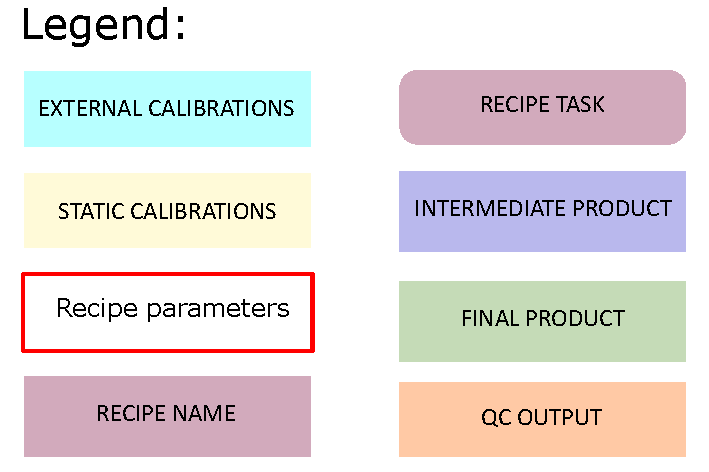
\includegraphics[width=0.4\textheight]{figures/legend.pdf}
  \caption[Legend]{Legend of the coloured boxes in the \ac{LSS} cascades.}
  \label{Fig:LSScascadelegend}
\end{figure}
\clearpage

\begin{sidewaysfigure}[ht]
  \centering
  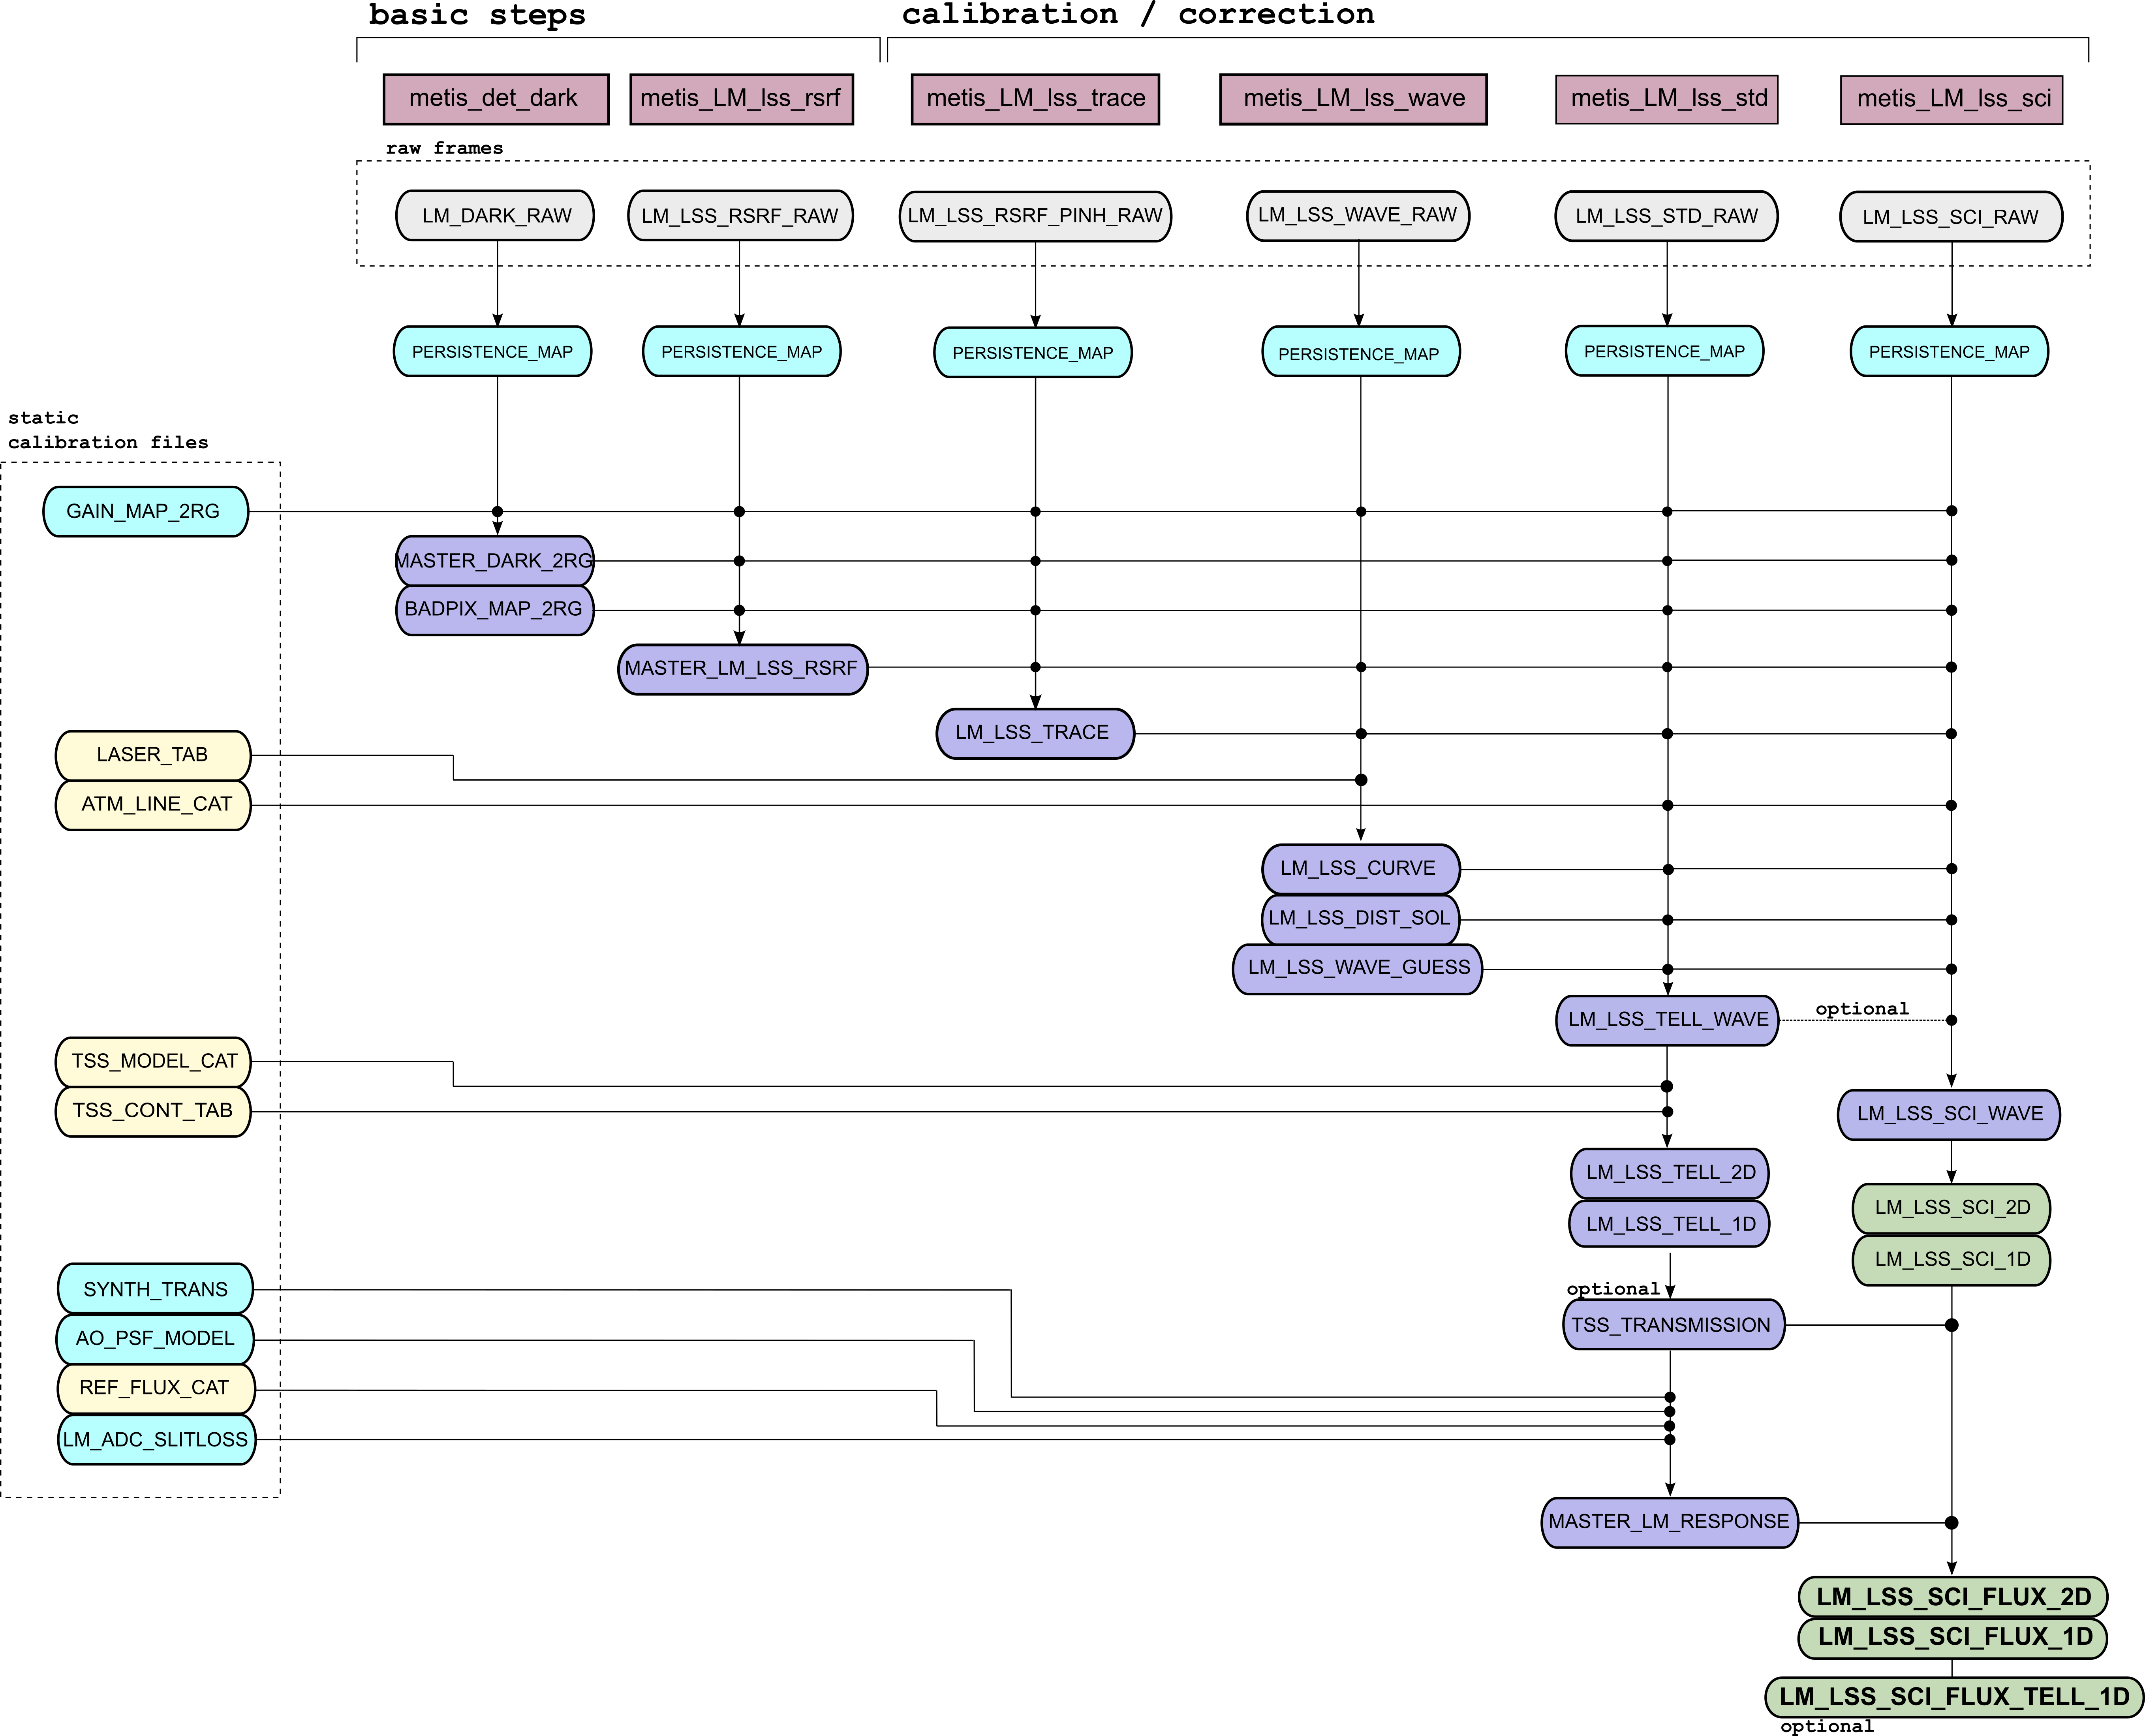
\includegraphics[width=0.9\textheight]{figures/LM_LSS_pipeline_wf_draft_latest_part_1_v0.80.png}
  \caption[Reduction cascade and association map for LM long-slit
  spectroscopy]{Part 1 of the reduction cascade and association map for long-slit
    spectroscopy in the LM bands.  }
  \label{Fig:LMLssAssomap1}
\end{sidewaysfigure}

\begin{sidewaysfigure}[ht]
  \centering
  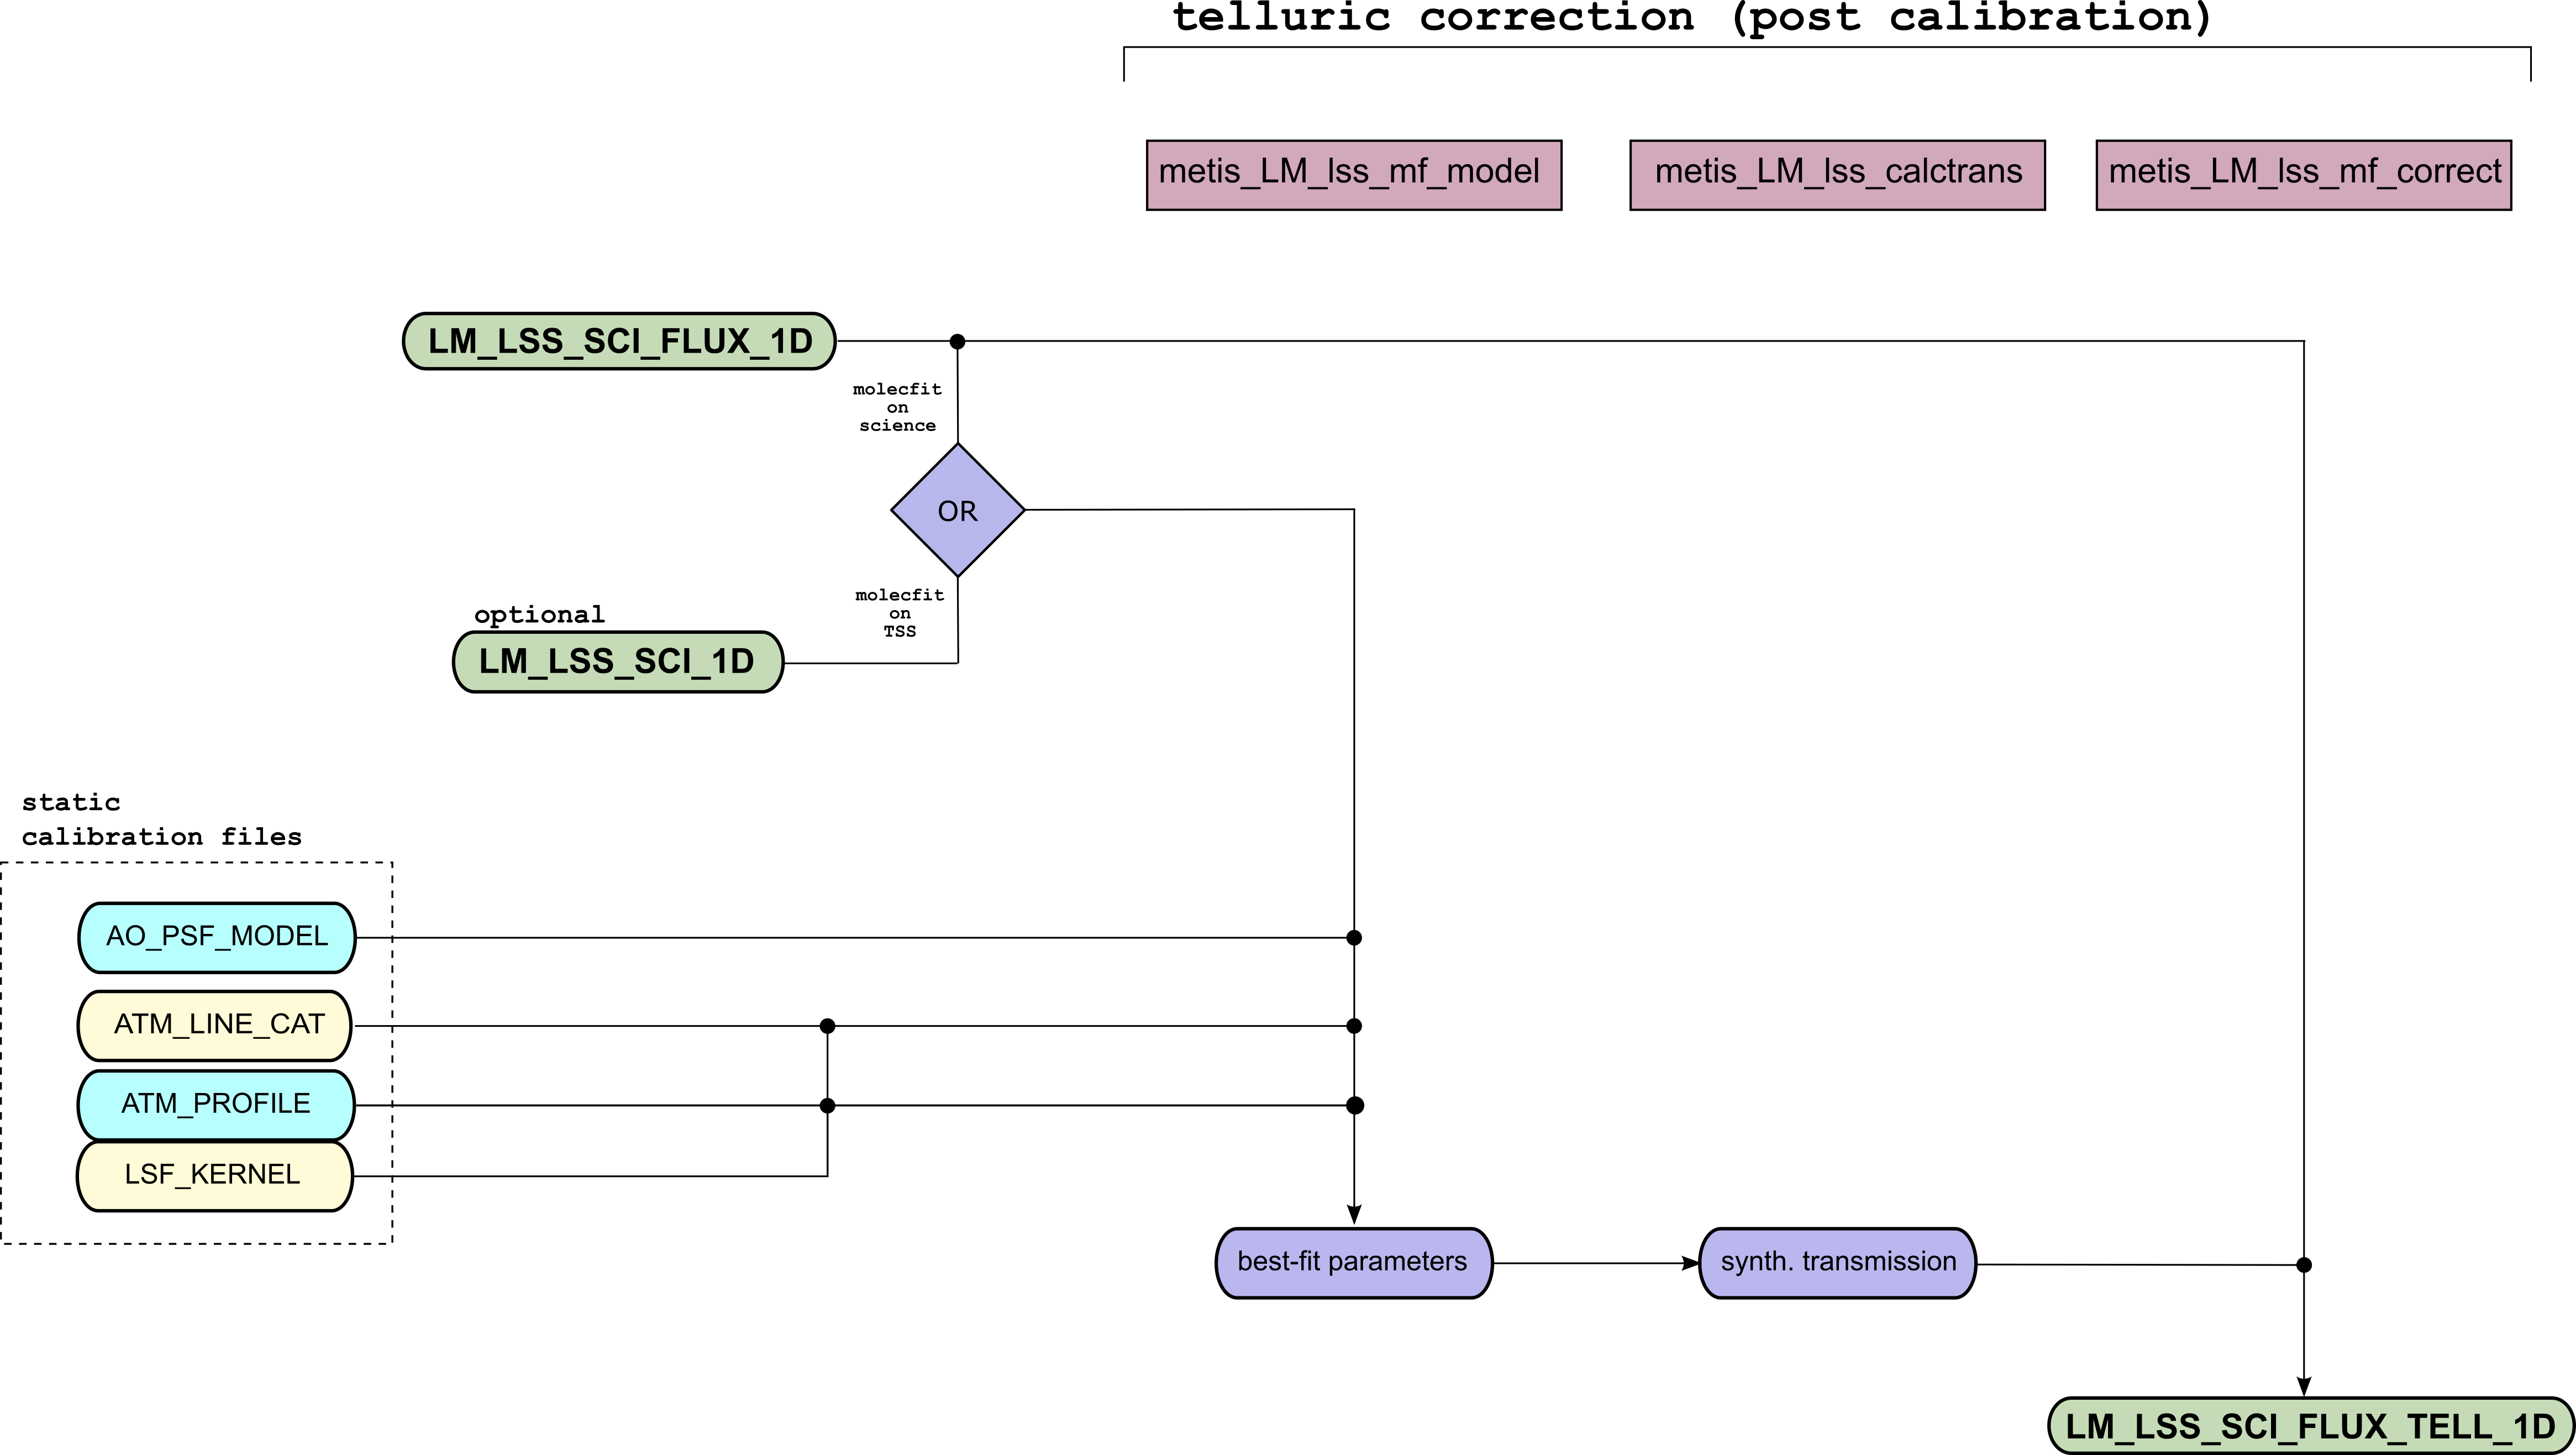
\includegraphics[width=0.8\textheight]{figures/LM_LSS_pipeline_wf_draft_latest_part_2_v0.80.png}
  \caption[Reduction cascade and association map for LM long-slit
  spectroscopy]{Part 2 of the reduction cascade and association map for long-slit
    spectroscopy in the LM bands.  }
  \label{Fig:LMLssAssomap2}
\end{sidewaysfigure}


% \begin{sidewaysfigure}[ht]
%   \centering
%   \includegraphics[width=0.9\textheight]{figures/NQ_LSS_pipeline_wf_draft_latest.png}
%   \caption[Reduction cascade and association map for N long-slit
%   spectroscopy]{Reduction cascade and association map for long-slit
%     spectroscopy in the N band.  }
%   \label{Fig:NQLssAssomap}
% \end{sidewaysfigure}


%% ---- Table: LM long-slit spectroscopy
\begin{sidewaystable}
  \footnotesize
  \begin{center}
    \caption[Data Processing table for LM long-slit spectroscopy]{%
      Data Processing table for LM long-slit spectroscopy
      calibration mode; }\bigskip
    \label{Tab:LMLssDatProc}
    \begin{tabular}{|l|l|l|l|l|l|}
      \hline
      Data Type   & Classification & Recipe (Level)	& FITS Keywords & static CalibDB & Products\\
    (Templates) & Keywords	 & Processing steps	&		&	  &	\\
    \hline
    \TPL{DARK}	& \CODE{DPR.CATG==CALIB} & \hyperref[sssec:metis_det_dark]{\REC{metis_det_dark}} & Exposure time	&	\hyperref[dataitem:gainmap2rg]{\PROD{GAIN_MAP_2RG}}& Averaged dark frame\\
    		& \CODE{DPR.TYPE==DARK}  &			&		&	& Bad pixel map\\
    		& \CODE{DPR.TECH==IMAGE}  &			&		&	& \\
    \hline
    \TPL{FLAT}	& \CODE{DPR.CATG==CALIB} & \hyperref[rec:lsslmrsrf]{\REC{metis_LM_lss_rsrf}} & Exposure time	& \hyperref[dataitem:gainmap2rg]{\PROD{GAIN_MAP_2RG}}	& Averaged, normalized flatfield\\
    		& \CODE{DPR.TYPE==FLAT}  &			&	Grism	& 	& \\
    		& \CODE{DPR.TECH==SPECTRUM}  &			&	Slit	&	& \\
    \hline
         	& \CODE{DPR.CATG==CALIB} &\hyperref[rec:lsslmtrace]{\REC{metis_LM_lss_trace}} & Exposure time	& \hyperref[dataitem:gainmap2rg]{\PROD{GAIN_MAP_2RG}}	& Order location\\
    		& \CODE{DPR.TYPE==FLAT}  &			&		&	& (polynomial fit)\\
    		& \CODE{DPR.TECH==SPECTRUM}  &			&		&	& \\
    \hline
    \TPL{WAVE,LASER} & \CODE{DPR.CATG==CATG} &\hyperref[rec:lsslmwave]{\REC{metis_LM_lss_wave}} & Exposure time &  \hyperref[dataitem:gainmap2rg]{\PROD{GAIN_MAP_2RG}} & wavelength solution\\
    		& \CODE{DPR.TYPE==WAVE,LASER}   &			   & Grism & \hyperref[dataitem:lasertab]{\STATCALIB{LASER_TAB}} &\\
    		& \CODE{DPR.TECH==SPECTRUM}  &			& Slit		&	& \\
    		& \CODE{PRO.CATG==SPECTRUM}   &  &  & & \\
    \hline
    \TPL{FLUX,STD} & \CODE{DPR.CATG==CALIB} & \hyperref[rec:lsslmstd]{\REC{metis_LM_lss_flux}}& Object name (Flux STD) & \hyperref[dataitem:gainmap2rg]{\PROD{GAIN_MAP_2RG}} & Instrumental\\
    		& \CODE{DPR.TYPE==FLUX,STD}   &			   & Exposure time & \hyperref[dataitem:atmlinecat]{\EXTCALIB{ATM_LINE_CAT}} & response function\\
    		& \CODE{DPR.TECH==SPECTRUM}  &			&	Grism	&	\hyperref[dataitem:lmsynthtrans]{\STATCALIB{LM_SYNTH_TRANS}}& \\
    		& \CODE{PRO.CATG==SPECTRUM}   &  & Slit & \hyperref[dataitem:lmadcslitloss]{\STATCALIB{LM_ADC_SLITLOSS}} & \\
    		& & & & \hyperref[dataitem:aopsfmodel]{\EXTCALIB{AO_PSF_MODEL}} &\\    
    		& & & & \hyperref[dataitem:reffluxcat]{\STATCALIB{REF_FLUX_CAT}} &\\    \hline
    \TPL{SCIENCE} & \CODE{DPR.CATG==SCIENCE} & \hyperref[rec:lsslmsci]{\REC{metis_LM_lss_sci}} & Object name &  \hyperref[dataitem:gainmap2rg]{\PROD{GAIN_MAP_2RG}} & Science grade spectrum\\
    		& \CODE{DPR.TYPE==OBJECT}   &			   & Exposure time & \hyperref[dataitem:lmadcslitloss]{\STATCALIB{LM_ADC_SLITLOSS}} &\\
    		& \CODE{DPR.TECH==SPECTRUM}  &			&	Grism	& \hyperref[dataitem:atmlinecat]{\EXTCALIB{ATM_LINE_CAT}}	& \\
    		& \CODE{PRO.CATG==SPECTRUM}   &  & Slit  &  & \\
    \hline
            & \CODE{DPR.CATG==SCIENCE} & \hyperref[rec:LMLSSmfmodel]{\REC{metis_LM_lss_mf_model}} & Object name & \hyperref[dataitem:lsfkernel]{\STATCALIB{LSF_KERNEL}}	 & Best-fit \\
    		& \CODE{DPR.TYPE==OBJECT}   &			  & & \hyperref[dataitem:atmprofile]{\EXTCALIB{ATM_PROFILE}}  & \texttt{molecfit} parameters\\
    		& \CODE{DPR.TECH==TBD}  &			&		& \hyperref[dataitem:atmlinecat]{\EXTCALIB{ATM_LINE_CAT}}	& \\
    		& \CODE{PRO.CATG==TBD}   &  &  & start parameter set & \\
    \hline
            & \CODE{DPR.CATG==SCIENCE} &  \hyperref[rec:LMLSSmfcalctrans]{\REC{metis_LM_lss_mf_calctrans}} & Object name & \hyperref[dataitem:atmlinecat]{\EXTCALIB{ATM_LINE_CAT}}	 & synthetic \\
    		& \CODE{DPR.TYPE==LSS}   &		&	   &   & Transmission curve\\
    		& \CODE{DPR.TECH==TBD}  &			&		& 	& \\
    		& \CODE{PRO.CATG==TBD}   &  &  & & \\
    \hline
            & \CODE{DPR.CATG==SCIENCE} &  \hyperref[rec:LMLSSmfcorrect]{\REC{metis_LM_lss_mf_correct}} & Object name & 	 & Absorption corrected\\
    		& \CODE{DPR.TYPE==LSS}   &			   & & synthetic Transmission curve  & science spectrum\\
    		& \CODE{DPR.TECH==TBD}  &			&		&	& \\
    		& \CODE{PRO.CATG==TBD}   &  &  & & \\
    \hline
    \end{tabular}
  \end{center}
\end{sidewaystable}

\begin{sidewaysfigure}[ht]
  \centering
  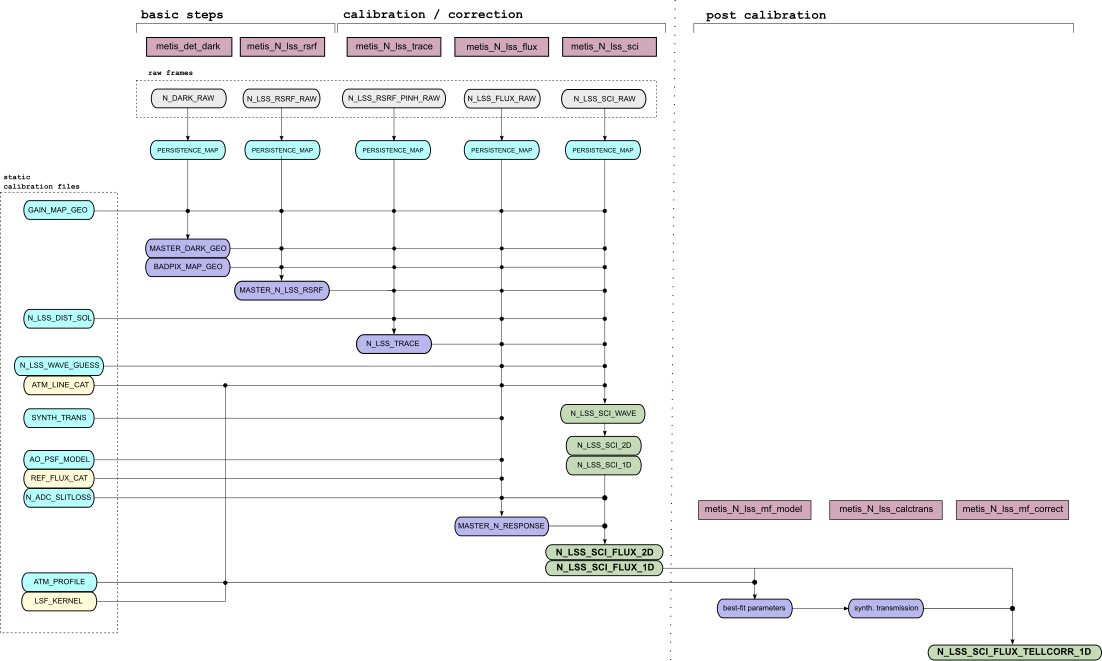
\includegraphics[width=0.9\textheight]{figures/N_LSS_pipeline_wf_draft_latest_v0.74.png}
  \caption[Reduction cascade and association map for N long-slit
  spectroscopy]{Reduction cascade and association map for long-slit
    spectroscopy in the N bands. }
  \label{Fig:NLssAssomap}
\end{sidewaysfigure}

%% ---- Table: N long-slit spectroscopy
\begin{sidewaystable}
  \footnotesize
  \begin{center}
    \caption[Data Processing table for N-band long-slit spectroscopy]{%
      Data Processing table for N long-slit spectroscopy
      calibration mode}\bigskip
    \label{Tab:NLssDatProc}
    \begin{tabular}{|l|l|l|l|l|l|}
      \hline
      Data Type   & Classification & Recipe (Level)	& FITS Keywords & static CalibDB & Products\\
    (Templates) & Keywords	 & Processing steps	&		&	  &	\\
    \hline
    \TPL{DARK}	& \CODE{DPR.CATG==CALIB} & \hyperref[sssec:metis_det_dark]{\REC{metis_det_dark}} & Exposure time	& \hyperref[dataitem:gainmap2rg]{\PROD{GAIN_MAP_GEO}}	& Averaged dark frame\\
    		& \CODE{DPR.TYPE==DARK}  &			&		&	& Bad pixel map\\
    		& \CODE{DPR.TECH==IMAGE}  &			&		&	& \\
    \hline
    \TPL{FLAT}	& \CODE{DPR.CATG==CALIB} & \hyperref[rec:lssnrsrf]{\REC{metis_N_lss_rsrf}} & Exposure time	& \hyperref[dataitem:gainmap2rg]{\PROD{GAIN_MAP_GEO}}	& Averaged, normalized flatfield (\ac{RSRF}\\
    		& \CODE{DPR.TYPE==FLAT}  &			&	Grism	&	& Bad pixel map\\
    		& \CODE{DPR.TECH==SPECTRUM}  &			& Slit		&	& \\
    \hline
         	& \CODE{DPR.CATG==CALIB} & \hyperref[rec:lssntrace]{\REC{metis_N_lss_trace} }& Exposure time	& \hyperref[dataitem:gainmap2rg]{\PROD{GAIN_MAP_GEO}}	& Order location\\
    		& \CODE{DPR.TYPE==FLAT}  &			&	Grism	&	& (polynomial fit)\\
    		& \CODE{DPR.TECH==SPECTRUM}  &			&	Slit	&	& \\
    \hline
    \TPL{FLUX,STD} & \CODE{DPR.CATG==CALIB} & \hyperref[rec:lssnflux]{\REC{metis_N_lss_flux}} & Object name (Flux STD) & \hyperref[dataitem:gainmap2rg]{\PROD{GAIN_MAP_GEO}} & Instrumental\\
    		& \CODE{DPR.TYPE==FLUX,STD}   &			   & Exposure time & \hyperref[dataitem:nlsswaveguess]{\STATCALIB{N_LSS_WAVE_GUESS}} & response function\\
    		& \CODE{DPR.TECH==SPECTRUM}   &			   & Grism		& \hyperref[dataitem:atmlinecat]{\EXTCALIB{ATM_LINE_CAT}}	& \\
    		& \CODE{PRO.CATG==SPECTRUM}   &  &  Slit & \hyperref[dataitem:nsynthtrans]{\STATCALIB{N_SYNTH_TRANS}} & \\
    		& & & & \hyperref[dataitem:nadcslitloss]{\STATCALIB{N_ADC_SLITLOSS}} &\\
    		& & & &  \hyperref[dataitem:reffluxcat]{\STATCALIB{REF_FLUX_CAT}} &\\
    		& & & & \hyperref[dataitem:aopsfmodel]{\EXTCALIB{AO_PSF_MODEL}} &\\
    		& & & & \hyperref[dataitem:nlssdistsol]{\STATCALIB{N_LSS_DIST_SOL}} &\\
    		& & & & \hyperref[dataitem:reffluxcat]{\STATCALIB{REF_FLUX_CAT}} &\\
    \hline
    \TPL{SCIENCE} & \CODE{DPR.CATG==SCIENCE} & \hyperref[rec:lssnsci]{\REC{metis_N_lss_sci}} & Object name & \hyperref[dataitem:gainmap2rg]{\PROD{GAIN_MAP_GEO}}  & Science grade spectrum\\
    		& \CODE{DPR.TYPE==OBJECT}   &			   & Exposure time &  \hyperref[dataitem:atmlinecat]{\EXTCALIB{ATM_LINE_CAT}} &\\
    		& \CODE{DPR.TECH==SPECTRUM}  &			&	Grism	&\hyperref[dataitem:nadcslitloss]{\STATCALIB{N_ADC_SLITLOSS}}	& \\
    		& \CODE{PRO.CATG==SPECTRUM}   &  & Slit & \hyperref[dataitem:nlsswaveguess]{\STATCALIB{N_LSS_WAVE_GUESS}} & \\
    		& & & & \hyperref[dataitem:nlssdistsol]{\STATCALIB{N_LSS_DIST_SOL}} &\\
    \hline
            & \CODE{DPR.CATG==SCIENCE} & \hyperref[rec:NLSSmfmodel]{\REC{metis_N_lss_mf_model}} & Object name & \hyperref[dataitem:lsfkernel]{\STATCALIB{LSF_KERNEL}}	 & Best-fit \\
    		& \CODE{DPR.TYPE==OBJECT}   &			  & & \hyperref[dataitem:atmprofile]{\EXTCALIB{ATM_PROFILE}}  & \texttt{molecfit} parameters\\
    		& \CODE{DPR.TECH==TBD}  &			&		& \hyperref[dataitem:atmlinecat]{\EXTCALIB{ATM_LINE_CAT}}	& \\
    		& \CODE{PRO.CATG==TBD}   &  &  & start parameter set & \\
    \hline
            & \CODE{DPR.CATG==SCIENCE} & \hyperref[rec:NLSSmfcalctrans]{\REC{metis_N_lss_mf_calctrans}} & Object name & \hyperref[dataitem:atmlinecat]{\EXTCALIB{ATM_LINE_CAT}}	 & synthetic \\
    		& \CODE{DPR.TYPE==LSS}   &		&	   &  & Transmission curve\\
    		& \CODE{DPR.TECH==TBD}  &			&		&  	& \\
    		& \CODE{PRO.CATG==TBD}   &  &  & & \\
    \hline
            & \CODE{DPR.CATG==SCIENCE} & \hyperref[rec:NLSSmfcorrect]{\REC{metis_N_lss_mf_correct}} & Object name & 	 & Absorption corrected\\
    		& \CODE{DPR.TYPE==LSS}   &			   &  & synthetic Transmission curve & science spectrum\\
    		& \CODE{DPR.TECH==TBD}  &			&		&	& \\
    		& \CODE{PRO.CATG==TBD}   &  &  & & \\
    \hline
    \end{tabular}
  \end{center}
\end{sidewaystable}

\subsubsection{Static calibration database}\label{lss:static_calib}
The static calibration database comprises several data sets, some are updated from time to time:
\begin{itemize}
    \item \hyperref[dataitem:gainmap2rg]{\hyperref[dataitem:gainmap2rg]{\PROD{GAIN_MAP_2RG}}} and \hyperref[dataitem:gainmapgeo]{\hyperref[dataitem:gainmap2rg]{\PROD{GAIN_MAP_GEO}}}: These are the detector gain maps of the detectors (2RG=Hawaii2RG, LM-band; GEO=Geosnap, N-band), which are created by the recipe \hyperref[sssec:metis_det_lingain]{\REC{metis_det_lingain}} (see Section~\ref{sssec:metis_det_lingain}). This recipe also checks the linearity of the pixels and is carried out every once in a while (yearly, TBD, see \cite{METIS-calibration_plan}) as we assume the detectors to be fairly stable.
    \item \hyperref[dataitem:lasertab]{\STATCALIB{LASER_TAB}}: The \ac{WCU} provides laser sources for the first guess of the wavelength solution. The main laser frequencies are fixed (\cite{METIS-calibration_plan}) and given in a static table.
    \item \hyperref[dataitem:atmlinecat]{\EXTCALIB{ATM_LINE_CAT}}: The main wavelength calibration will be done by means of atmospheric lines, most probably based on the \ac{HITRAN}\footnote{\url{https://hitran.org/}}. They are given in a static catalogue. This database is also required by the telluric correction package \texttt{molecfit}.
    \item \hyperref[dataitem:lmsynthtrans]{\STATCALIB{LM_SYNTH_TRANS}}/\hyperref[dataitem:nsynthtrans]{\STATCALIB{N_SYNTH_TRANS}}: For the determination of the continuum of flux standard stars a rough telluric correction is needed. We intend to apply static transmission curves for that purpose as we deem it to be sufficient and more time efficient than applying the telluric correction package \texttt{molecfit} every time. This static transmission curve will be determined during commissioning via \texttt{molecfit}.
    \item \hyperref[dataitem:aopsfmodel]{\EXTCALIB{AO_PSF_MODEL}}: For the determination of \ac{AO}-induced slit losses we intend to use a static \ac{PSF} model, which is scaled by the \ac{AO} telemetry data. Details on that are TBD.
    \item \hyperref[dataitem:reffluxcat]{\STATCALIB{REF_FLUX_CAT}}: The absolute flux calibration will be done by observations of specific flux standard stars, which are compared to their theoretical models. The \hyperref[dataitem:reffluxcat]{\STATCALIB{REF_FLUX_CAT}} will contain these models. Currently, the catalogue of flux standard stars comprises the stars from the catalogue of the \ac{VISIR} instrument.

    \item \hyperref[dataitem:tssmodelcat]{\STATCALIB{TSS_MODEL_CAT}}: In some cases, the default modelling method for the telluric correction might not be possible or leading to bad results. We therefore foresee the possibility to use telluric standard stars. For the determination of the transmisison function a model of the selected telluric star is required. In this table, a model of a set of such stars
    \item \hyperref[dataitem:tssconttab]{\STATCALIB{TSS_CONT_TAB}}: 

    \item \hyperref[dataitem:lmadcslitloss]{\STATCALIB{LM_ADC_SLITLOSS}}/\hyperref[dataitem:nadcslitloss]{\STATCALIB{N_ADC_SLITLOSS}}: It is expected that the fixed positions of the \ac{ADC} will introduce specific slit losses. These losses are determined in the recipes \hyperref[rec:metislmadcmslitloss]{\REC{metis_lm_adc_slitloss}} and \hyperref[rec:metisnadcmslitloss]{\REC{metis_n_adc_slitloss}} (see Section~\ref{sssec:adc_slitlosses} and \cite{METIS-calibration_plan}). As these losses are assumed to be very stable, these recipes will be carried out only rarely.
    \item \hyperref[dataitem:atmprofile]{\EXTCALIB{ATM_PROFILE}} and \hyperref[dataitem:lsfkernel]{\STATCALIB{LSF_KERNEL}}: The telluric correction package \texttt{molecfit} requires an atmospheric profile incorporating height information of the temperature, pressure and molecular abundances as input. Currently we use a static profile (equatorial \texttt{equ.atm}\footnote{\url{https://eodg.atm.ox.ac.uk/RFM/atm/}}) as starting point of the fit of the molecular column densities. In addition, a kernel for the \ac{LSF} is provided. We intend to determine the kernel during commissioning and use this as input. However, it is still unclear in how far the \ac{AO} influences that kernel. The current baseline is to use the static \hyperref[dataitem:lsfkernel]{\STATCALIB{LSF_KERNEL}} as starting point for fitting the line spread function.
    \item \hyperref[dataitem:nlssdistsol]{\STATCALIB{N_LSS_DIST_SOL}}/\hyperref[dataitem:nlsswaveguess]{\STATCALIB{N_LSS_WAVE_GUESS}}: First guess solutions of the N-band LSS mode are static due to the absence of laser sources after \ac{AIT}. As the instrument is expected to be very stable, these calibration files will be created only once and kept static.
\end{itemize}  % TO BE EDITED BY INNSBRUCK ONLY!!!!!

\clearpage
% IFU-mode
% \input{05_3-Overview_IFU}

\section{Pipeline Recipes}
\label{sec:pipeline_recipes}

% \input{06_1a-Recipes_Detector}
% \newpage
% \input{06_1b-Recipes_Imaging_LM}
% \input{06_2-Recipes_Imaging_NQ}
\clearpage
\subsection{Long-slit spectroscopy, LM band}
\label{ssec:recipes_lss_lm}

A draft of the reduction cascade is shown in
Figs.~\ref{Fig:LMLssAssomap1} and \ref{Fig:LMLssAssomap2} together with the data processing table
(Tables~\ref{Tab:LMLssDatProc1} and ~\ref{Tab:LMLssDatProc2}). The first part aims to update the static calibration database, in particular the creation of the gain map (\hyperref[Sec:detector_calibration]{\REC{metis_det_lingain}}) and the determination of the \ac{ADC} slitlosses (\hyperref[rec:metis_lm_adc_slitloss]{\REC{metis_lm_adc_slitloss}}). These are executed only when an update is required, e.g. after a major instrument interention or on yearly basis. The second part comprises the basic calibrations, e.g. the dark correction and the spectroscopic flatfielding via \ac{RSRF}, followed by the third part, the main calibration steps, incorporating the determination of the first guess wavelength solution by means of the laser sources in the \ac{WCU} and the determination of the response curve for the flux calibration. Subsequently, the main reduction is conducted, which applies the previously created master calibration files to the science frames. Both, the flux standard and the science observations are wavelength calibrated with the help of the atmospheric lines visible in the respective spectra. Therefore the main step of the wavelength calibration is carried out in the recipes \hyperref[rec:metis_lm_lss_std]{\REC{metis_LM_lss_std}} and \hyperref[rec:metis_lm_lss_sci]{\REC{metis_LM_lss_sci}}. Finally, the telluric absorption correction is applied using the modelling approach with \texttt{molecfit}. Optionally, the telluric correction can be done with a telluric standard star.


%------------------------------------------------------------------------------------------------------------------
\subsubsection{Recipes \REC{metis_det_lingain} and \REC{metis_det_dark}}
These recipes are described in Section~\ref{Sec:detector_calibration}.

%------------------------------------------------------------------------------------------------------------------
\subsubsection{Recipe \REC{metis_LM_adc_slitloss}}
The recipe \hyperref[sssec:adc_slitlosses]{\REC{metis_LM_adc_slitloss}} aims to determine the slit losses induced by the fixed \ac{ADC} positions as function of the object position across the slit. The recipe aims to create a table with slitlosses (\hyperref[dataitem:lm_adc_slitloss]{\STATCALIB{LM_ADC_SLITLOSS}}), which is added to the static database and used in the recipes \hyperref[rec:metis_lm_lss_std]{\REC{metis_LM_lss_std}}. This recipe is to be carried out only when an update of the database is needed. The algorithm and the workflow of the recipe to determine the slitlosses is given in Section~\ref{sssec:adc_slitlosses}, more information can be found in Section "Calibration of slit losses" in the Calibration Plan \cite{METIS-calibration_plan}. 


%------------------------------------------------------------------------------------------------------------------
\subsubsection{LM-LSS Flatfielding recipe \REC{metis_LM_lss_rsrf}:}\label{rec:metis_lm_lss_rsrf}
The recipe \hyperref[rec:metis_lm_lss_rsrf]{\REC{metis_LM_lss_rsrf}} aims to create a spectroscopic master flatfield for determining the pixel-to-pixel sensitivity and to enable the order location algorithm (\hyperref[rec:metis_lm_lss_trace]{\REC{metis_LM_lss_trace}}).
\begin{figure}[ht]
  \centering
  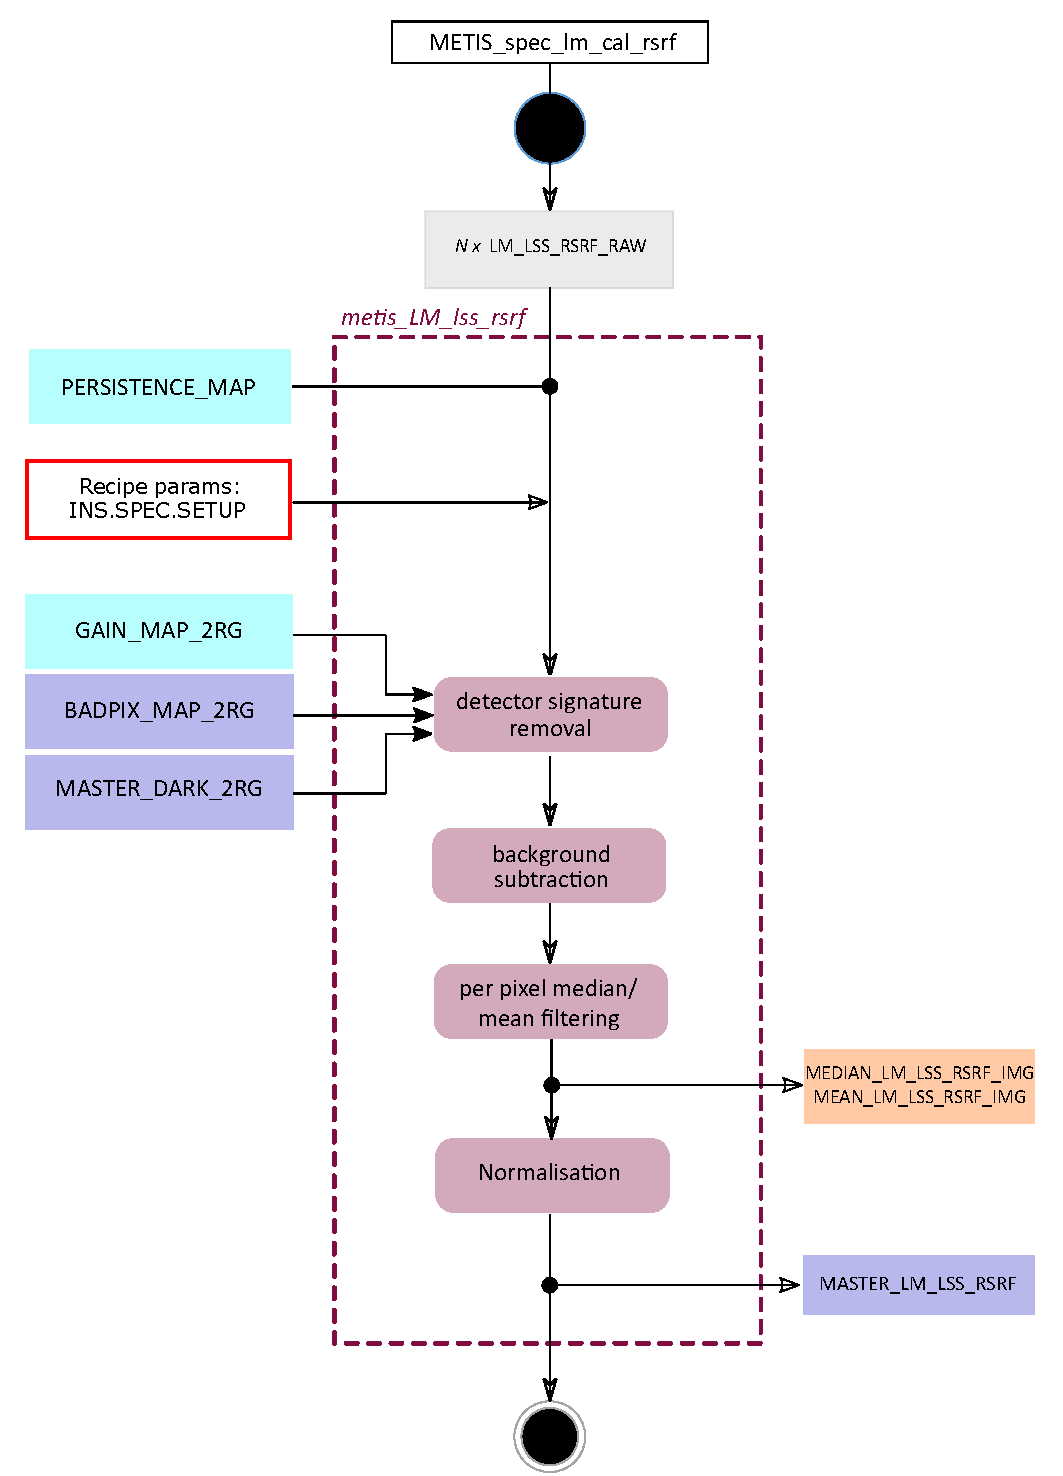
\includegraphics[width=0.5\textheight]{figures/metis_lm_lss_rsrf_v0.82.pdf}
  \caption[Recipe: \REC{metis_LM_lss_rsrf}]{\REC{metis_LM_lss_rsrf} --
    Recipe workflow to create the spectroscopic flatfield by means of the \ac{RSRF}.}
  \label{Fig:rec_lm_lss_rsrf}
\end{figure}

\begin{recipedef}
Name:		& \hyperref[rec:metis_lm_lss_rsrf]{\REC{metis_LM_lss_rsrf}}  \\
Purpose:	& Spectroscopic flatfielding with \ac{RSRF} \\
Type:		& Calibration\\
Requirements: & None \\
Templates:           & \TPL{METIS_spec_lm_cal_rsrf} \\
Input data:     & $N\times$ \hyperref[dataitem:lm_lss_rsrf_raw]{\RAW{LM_LSS_RSRF_RAW}} \\
                & \hyperref[dataitem:persistence_map]{\EXTCALIB{PERSISTENCE_MAP}}  \\
                & \hyperref[dataitem:gain_map_lm]{\STATCALIB{GAIN_MAP_LM}}  \\
                & \hyperref[dataitem:badpix_map_lm]{\PROD{BADPIX_MAP_LM}}  \\
                & \hyperref[dataitem:master_dark_lm]{\PROD{MASTER_DARK_LM}}  \\
Parameters: 	& TBD\\
Algorithm:      & subtract master \ac{WCU} "OFF" frame from illumination frame (done on individual images)\\
                & median/mean filtering of subtracted images\\
                & division by blackbody spectrum\\
                & normalisation to achieve \ac{RSRF}\\
Output data:	& \hyperref[dataitem:master_lm_lss_rsrf]{\PROD{MASTER_LM_LSS_RSRF}} (\FITS{PRO.CATG=MASTER_LM_LSS_RSRF}): \\
                & \hyperref[dataitem:median_lm_lss_rsrf_img]{\PROD{MEDIAN_LM_LSS_RSRF_IMG}}\\
                & \hyperref[dataitem:mean_lm_lss_rsrf_img]{\PROD{MEAN_LM_LSS_RSRF_IMG}}\\
Expected accuracies: & 3\% (cf. \cite{METIS-calibration_plan} and \cite{METIS_calerrbudget})\\
QC1 parameters: & \hyperref[qc:lmlssrsrfmeanlevel]{\QC{QC LM LSS RSRF MEAN LEVEL}}: Mean level of the \ac{RSRF}\\
                & \hyperref[qc:lmlssrsrfmedianlevel]{\QC{QC LM LSS RSRF MEDIAN LEVEL}}: Median level of the \ac{RSRF}\\
                & \hyperref[qc:lmlssrsrfintordrlevel]{\QC{QC LM LSS RSRF INTORDR LEVEL}}: Flux level of the interorder background\\
                & \hyperref[qc:lmlssrsrfnormstdev]{\QC{QC LM LSS RSRF NORM STDEV}}: Standard deviation of the normalised \ac{RSRF}\\
                & \hyperref[qc:lmlssrsrfnormsnr]{\QC{QC LM LSS RSRF NORM SNR}}: \ac{SNR} of the normalised \ac{RSRF}\\
                & more TBD\\
\end{recipedef}
\clearpage

%------------------------------------------------------------------------------------------------------------------
\subsubsection{LM-LSS Order detection \REC{metis_LM_lss_trace}:}\label{rec:metis_lm_lss_trace}
The recipe \hyperref[rec:metis_lm_lss_trace]{\REC{metis_LM_lss_trace}} aims at detecting the orders and a polynomial fitting of the order locations (see \cite{pis02} and \cite{pis21} for details on the algorithms). The detection and polynomial fitting is based on flatfield frames taken through a pinhole mask, which leads to individual pinhole traces along the entire dispersion direction.

\begin{figure}[ht]
  \centering
  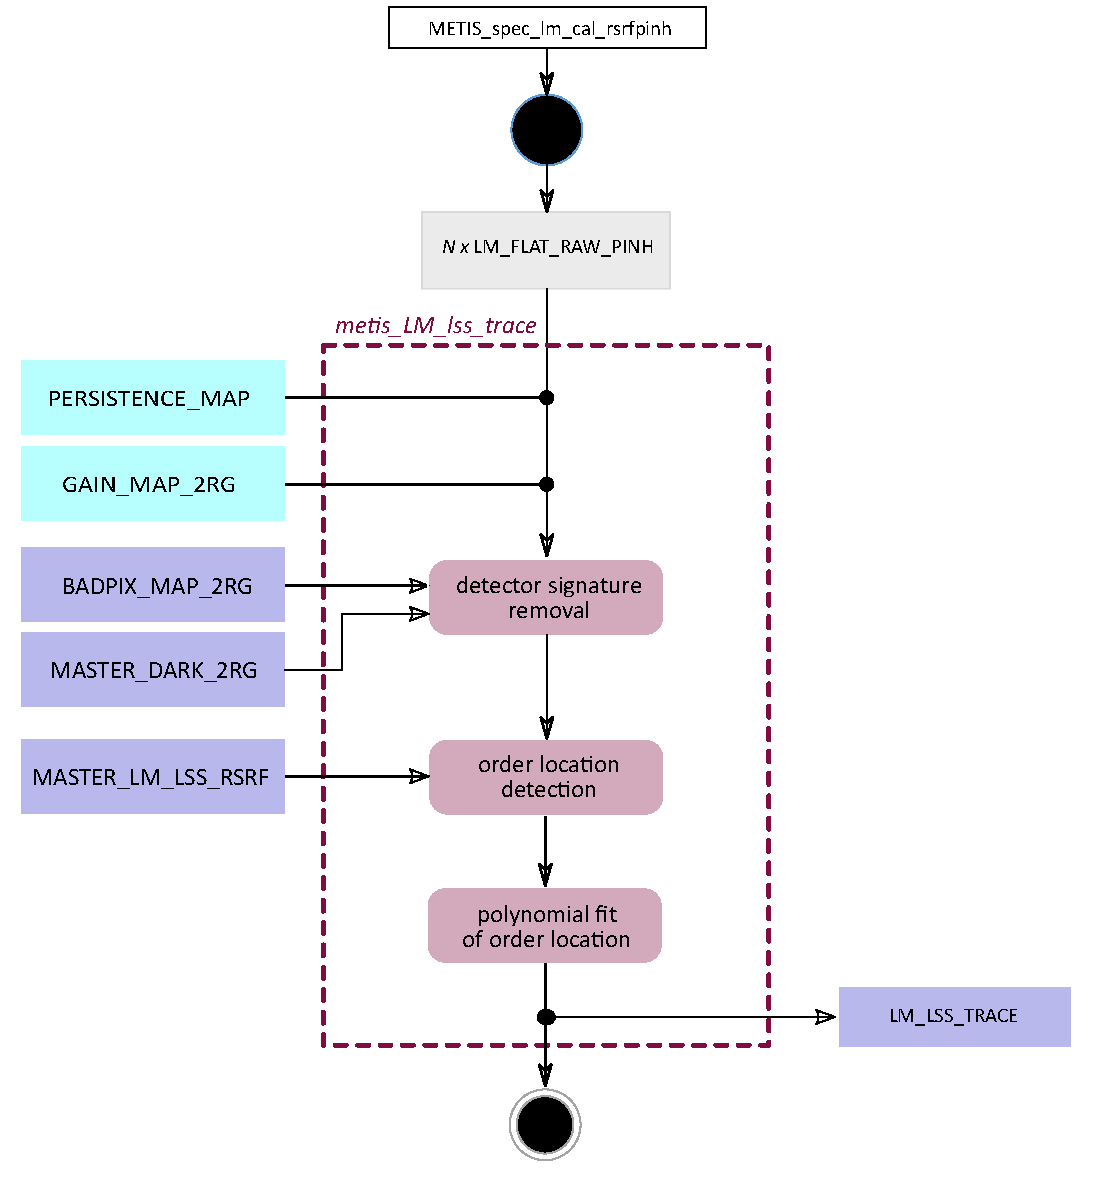
\includegraphics[width=0.5\textheight]{figures/metis_lm_lss_trace_v0.82.pdf}
  \caption[Recipe: \REC{metis_LM_lss_trace}]{\REC{metis_LM_lss_trace} --
    Detection and polynomial fitting of the order location.}
  \label{Fig:rec_lm_lss_wtrace}
\end{figure}

\begin{recipedef}
Name:		&  \hyperref[rec:metis_lm_lss_trace]{\REC{metis_LM_lss_trace}} \\
Purpose:	& Detection of order location \\
Type:		& Calibration\\
Requirements: & None \\
Templates:           & \TPL{METIS_spec_lm_cal_InternalWave}  \\
Input data:     & $N\times$ \hyperref[dataitem:lm_lss_rsrf_pinh_raw]{\RAW{LM_LSS_RSRF_PINH_RAW}} \\
                & \hyperref[dataitem:persistence_map]{\EXTCALIB{PERSISTENCE_MAP}}  \\
                & \hyperref[dataitem:gain_map_lm]{\STATCALIB{GAIN_MAP_LM}}  \\
                & \hyperref[dataitem:badpix_map_lm]{\PROD{BADPIX_MAP_LM}}  \\
                & \hyperref[dataitem:master_dark_lm]{\PROD{MASTER_DARK_LM}}  \\
                & \hyperref[dataitem:master_lm_lss_rsrf]{\PROD{MASTER_LM_LSS_RSRF}} \\
Parameters: 	& polynomial degree\\
Algorithm:      & Detection of the order edges\\
                & Polynomial fitting\\
Output data:	& \hyperref[dataitem:lm_lss_trace]{\PROD{LM_LSS_TRACE}} (\FITS{PRO.CATG=LM_LSS_TRACE}): Polynomial coefficients\\
Expected accuracies: & (TBD)\\
QC1 parameters: & \hyperref[qc:lmlsstracelpolydeg]{\QC{QC LM LSS TRACE LPOLYDEG}}: Degree of the polynomial fit of the left order edge\\
                & \hyperref[qc:lmlsstracelcoeffi]{\QC{QC LM LSS TRACE LCOEFF<i>}}: $i$-th coefficient of the polynomial of the left order edge\\
                & \hyperref[qc:lmlsstracerpolydeg]{\QC{QC LM LSS TRACE RPOLYDEG}}: Degree of the polynomial fit of the right order edge\\
                & \hyperref[qc:lmlsstracercoeffi]{\QC{QC LM LSS TRACE RCOEFF<i>}}: $i$-th coefficient of the polynomial of the right order edge\\
                & \hyperref[qc:lmlsstraceintrordrlevel]{\QC{QC LM LSS TRACE INTORDR LEVEL}}: Flux level of the interorder background\\
                & more TBD\\
\end{recipedef}

\clearpage
%------------------------------------------------------------------------------------------------------------------
\subsubsection{LM-LSS wavelength calibration recipe \REC{metis_LM_lss_wave}:}\label{rec:metis_lm_lss_wave}
This recipe aims at determining the first guess of the wavelength calibration on basis of the \ac{WCU} laser sources (c.f. \cite{METIS-calibration_plan}). Therefore the first steps are the removal of the detector signature of the \FITS{LM_WAVE_RAW} frames by applying the master calibration files derived in the previous steps, following by the background subtraction (if needed, TBD) and the application of the RSRF. The distortion of the lines (i.e. possible tilt, curvature,...) and the wavelength solution is determined by the algorithm developed by Piskunov et al. (\cite{pis02}, \cite{pis21}). The reference frame is defined by the laser line catalogue (\hyperref[dataitem:laser_tab]{\STATCALIB{LASER_TAB}}).

 This is in compliance with \REQ{METIS-6074}.

\begin{figure}[ht]
  \centering
  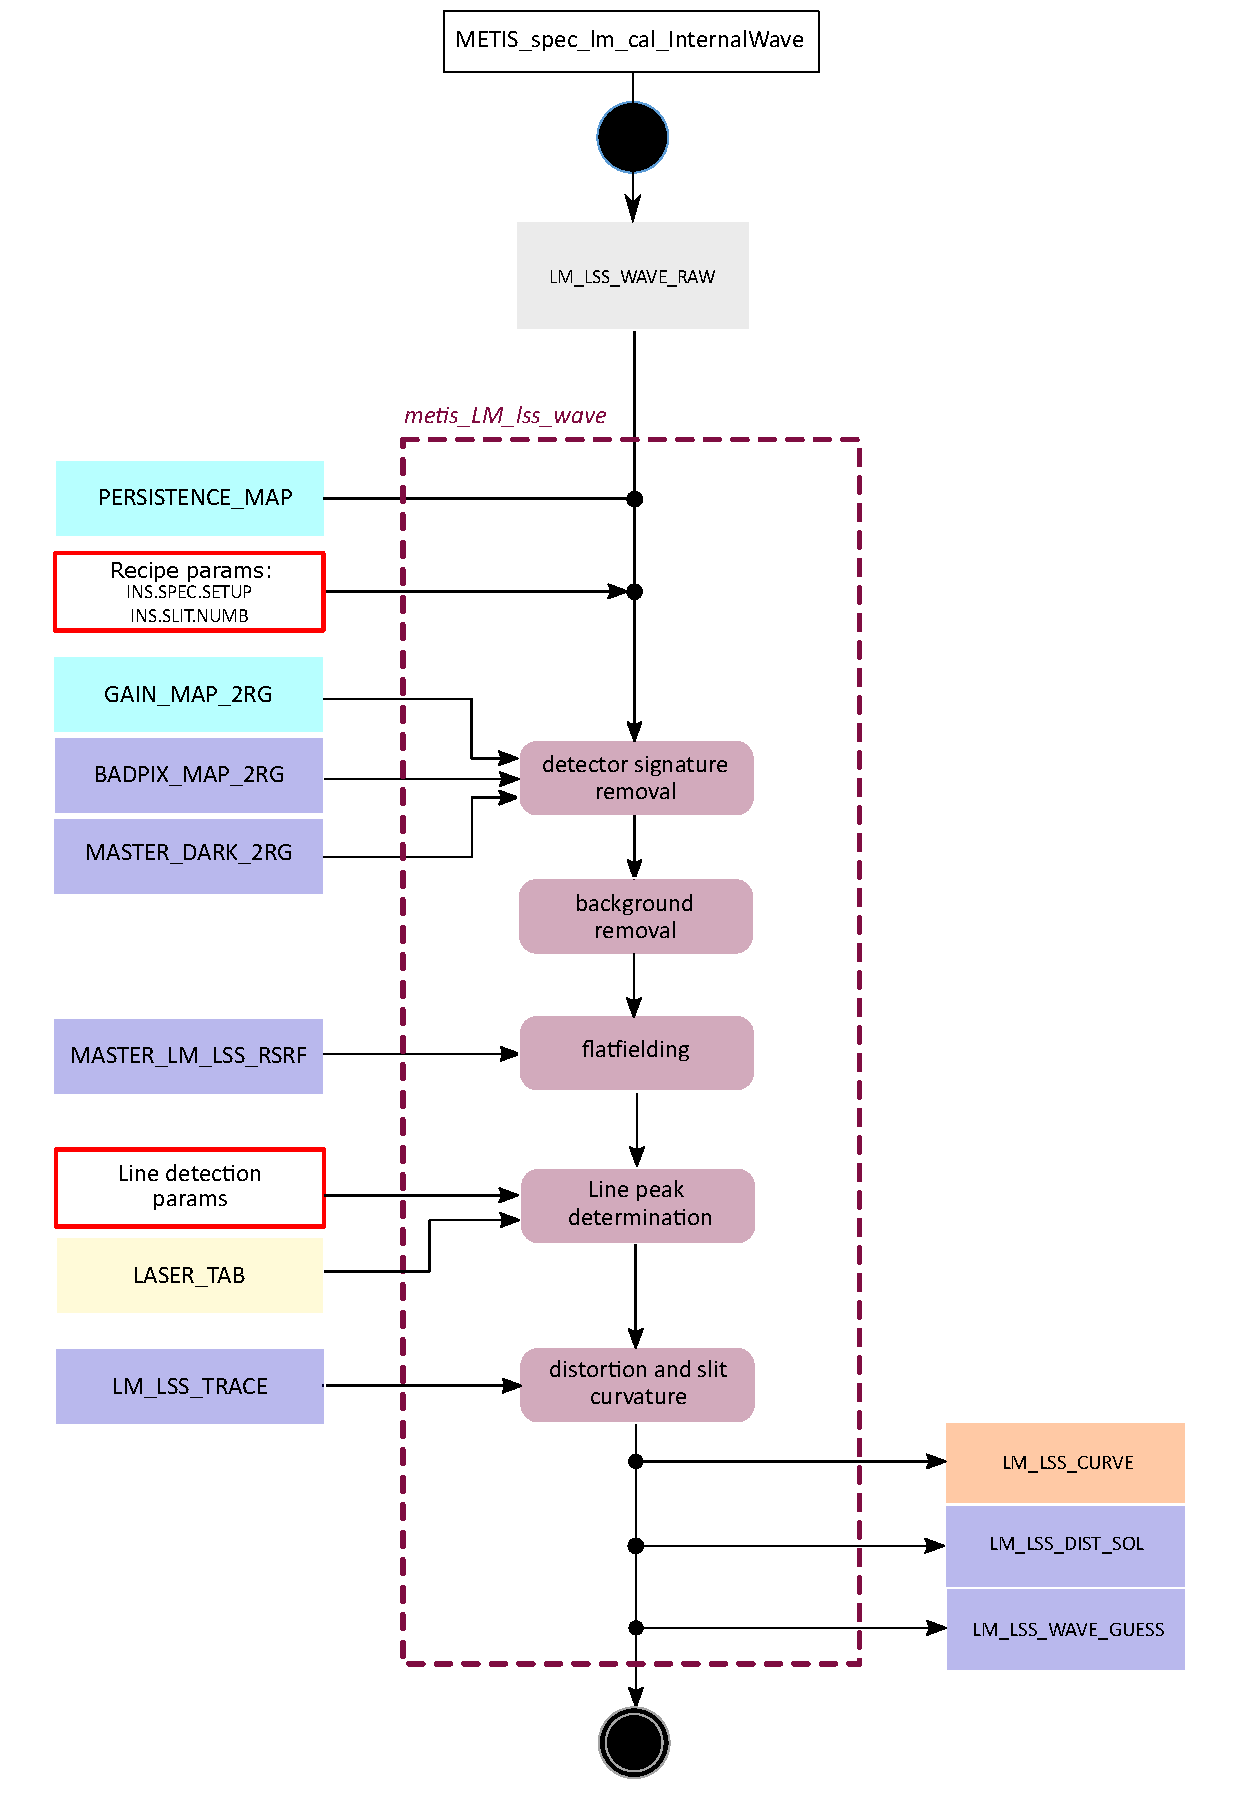
\includegraphics[width=0.5\textheight]{figures/metis_lm_lss_wave_v0.82.pdf}
  \caption[Recipe: \REC{metis_LM_lss_wave}]{\REC{metis_LM_lss_wave} --
    Creation of the LM LSS master wavelength correction.}
  \label{Fig:rec_lm_lss_trace}
\end{figure}
\clearpage

\begin{recipedef}
Name:		& \hyperref[rec:metis_lm_lss_wave]{\REC{metis_LM_lss_wave}} \\
Purpose:	& Wavelength calibration \\
Type:		& Calibration\\
Requirements: & METIS-6084, METIS-1371, METIS-6074 \\
Templates:           & \TPL{METIS_spec_lm_cal_internalwave}, \\
Input data: 	& \hyperref[dataitem:lm_lss_wave_raw]{\RAW{LM_LSS_WAVE_RAW}}\\
                & \hyperref[dataitem:persistence_map]{\EXTCALIB{PERSISTENCE_MAP}}  \\
                & \hyperref[dataitem:gain_map_lm]{\STATCALIB{GAIN_MAP_LM}}  \\
                & \hyperref[dataitem:badpix_map_lm]{\PROD{BADPIX_MAP_LM}}  \\
                & \hyperref[dataitem:master_dark_lm]{\PROD{MASTER_DARK_LM}}  \\
                & \hyperref[dataitem:master_lm_lss_rsrf]{\PROD{MASTER_LM_LSS_RSRF}} \\
                & \hyperref[dataitem:lm_lss_trace]{\PROD{LM_LSS_TRACE}} \\
                & \hyperref[dataitem:laser_tab]{\STATCALIB{LASER_TAB}} \\
                % & \hyperref[dataitem:ref_airg_cat]{\STATCALIB{REF_AIRG_CAT}} \\
Parameters: 	& (TBD)\\
Algorithm:      & Application of detector master calibration files\\
                & Determination and application of the distortion correction\\
                & Determination of the first guess of the wavelength solution by polynomial fit of the detected laser source lines\\
Output data:	& \hyperref[dataitem:lm_lss_curve]{\PROD{LM_LSS_CURVE}} (\FITS{PRO.CATG=LM_LSS_CURVE}): Curvature \\
                & \hyperref[dataitem:lm_lss_dist_sol]{\PROD{LM_LSS_DIST_SOL}} (\FITS{PRO.CATG=LM_LSS_DIST_SOL}): Distortion solution\\
                & \hyperref[dataitem:lm_lss_wave_guess]{\PROD{LM_LSS_WAVE_GUESS}} (\FITS{PRO.CATG=LM_LSS_WAVE_GUESS}): Wavelength first guess\\
Expected accuracies: & 1/5th of a pixel after post-processing (cf. \cite{METIS-calibration_plan})\\
QC1 parameters: & \hyperref[qc:lmlsswavepolydeg]{\QC{QC LM LSS WAVE POLYDEG}}: Degree of the first guess polynomial\\
                & \hyperref[qc:lmlsswavecoeffi]{\QC{QC LM LSS WAVE COEFF<i>}}: $i$-th coefficient of the polynomial\\
                & \hyperref[qc:lmlsswavenlines]{\QC{QC LM LSS WAVE NLINES}}: Number of detected (laser) lines; should be constant\\
                & \hyperref[qc:lmlsswavelinefwhmavg]{\QC{QC LM LSS WAVE LINEFWHMAVG}}: Average of the \ac{FWHM} of the detected lines (should be widely constant)\\
                & \hyperref[qc:lmlsswaveinterordrlevel]{\QC{QC LM LSS WAVE INTORDR LEVEL}}: Flux level of the interorder background\\
                & more TBD: e.g. QC params for distortion determination and correction\\
\end{recipedef}

\clearpage
%------------------------------------------------------------------------------------------------------------------
\subsubsection{LM-LSS standard star calibration recipe \REC{metis_LM_lss_std}:}\label{rec:metis_lm_lss_std}
\TODO{Finish following text} 

This recipe aims at processing standard stars used for the absolute flux calibration and (optionally) for the telluric feature removal: As first step the detector master calibration files derived previously are applied followed by the background subtraction, if needed the distortion correction (\hyperref[dataitem:lm_lss_dist_sol]{\PROD{LM_LSS_DIST_SOL}}), and
the wavelength calibration by means of the first guess solution (\hyperref[dataitem:lm_lss_wave_guess]{\PROD{LM_LSS_WAVE_GUESS}}) and the telluric sky lines (c.f. Sect.\,8.5 in \cite{DRLS}). Then the recipe removes sky background, extracts the standard star spectrum object and collapses the 2D to 1D spectra. To better compare the corresponding model spectrum a telluric correction is required. This is done by means of the standard star observations itself or (optionally) with \texttt{molecfit}.\\
It is on the user's decision whether the standard star is used for the absolute flux calibration only, or also used for the telluric correction of the science target.

As one needs to determine the stellar continuum regions, a telluric correction is required to increase these regions. This can be done either by applying a fairly simple telluric correction in an automated way to the standard star spectrum. In case the the user decides to use the standard star also for the telluric correction, a transmission function is derived from that in the "classical" way (cf. Section~\ref{sssec:tecllcorrclassic}), which will be optionally used for the telluric correction also for the science target. This star spectrum can also be optionally used for the wavelength solution and for the flux calibration, if the \ac{TSS} is suited for that. The response curve is obtained by comparing the extracted spectrum with a model and/or another reference spectrum of the standard star. Currently it is foreseen to use the same standard stars as in \ac{CRIRES}/CRIRES+ and \ac{VISIR}. It is under investigation whether more stars are needed.
\begin{figure}[ht]
  \centering
  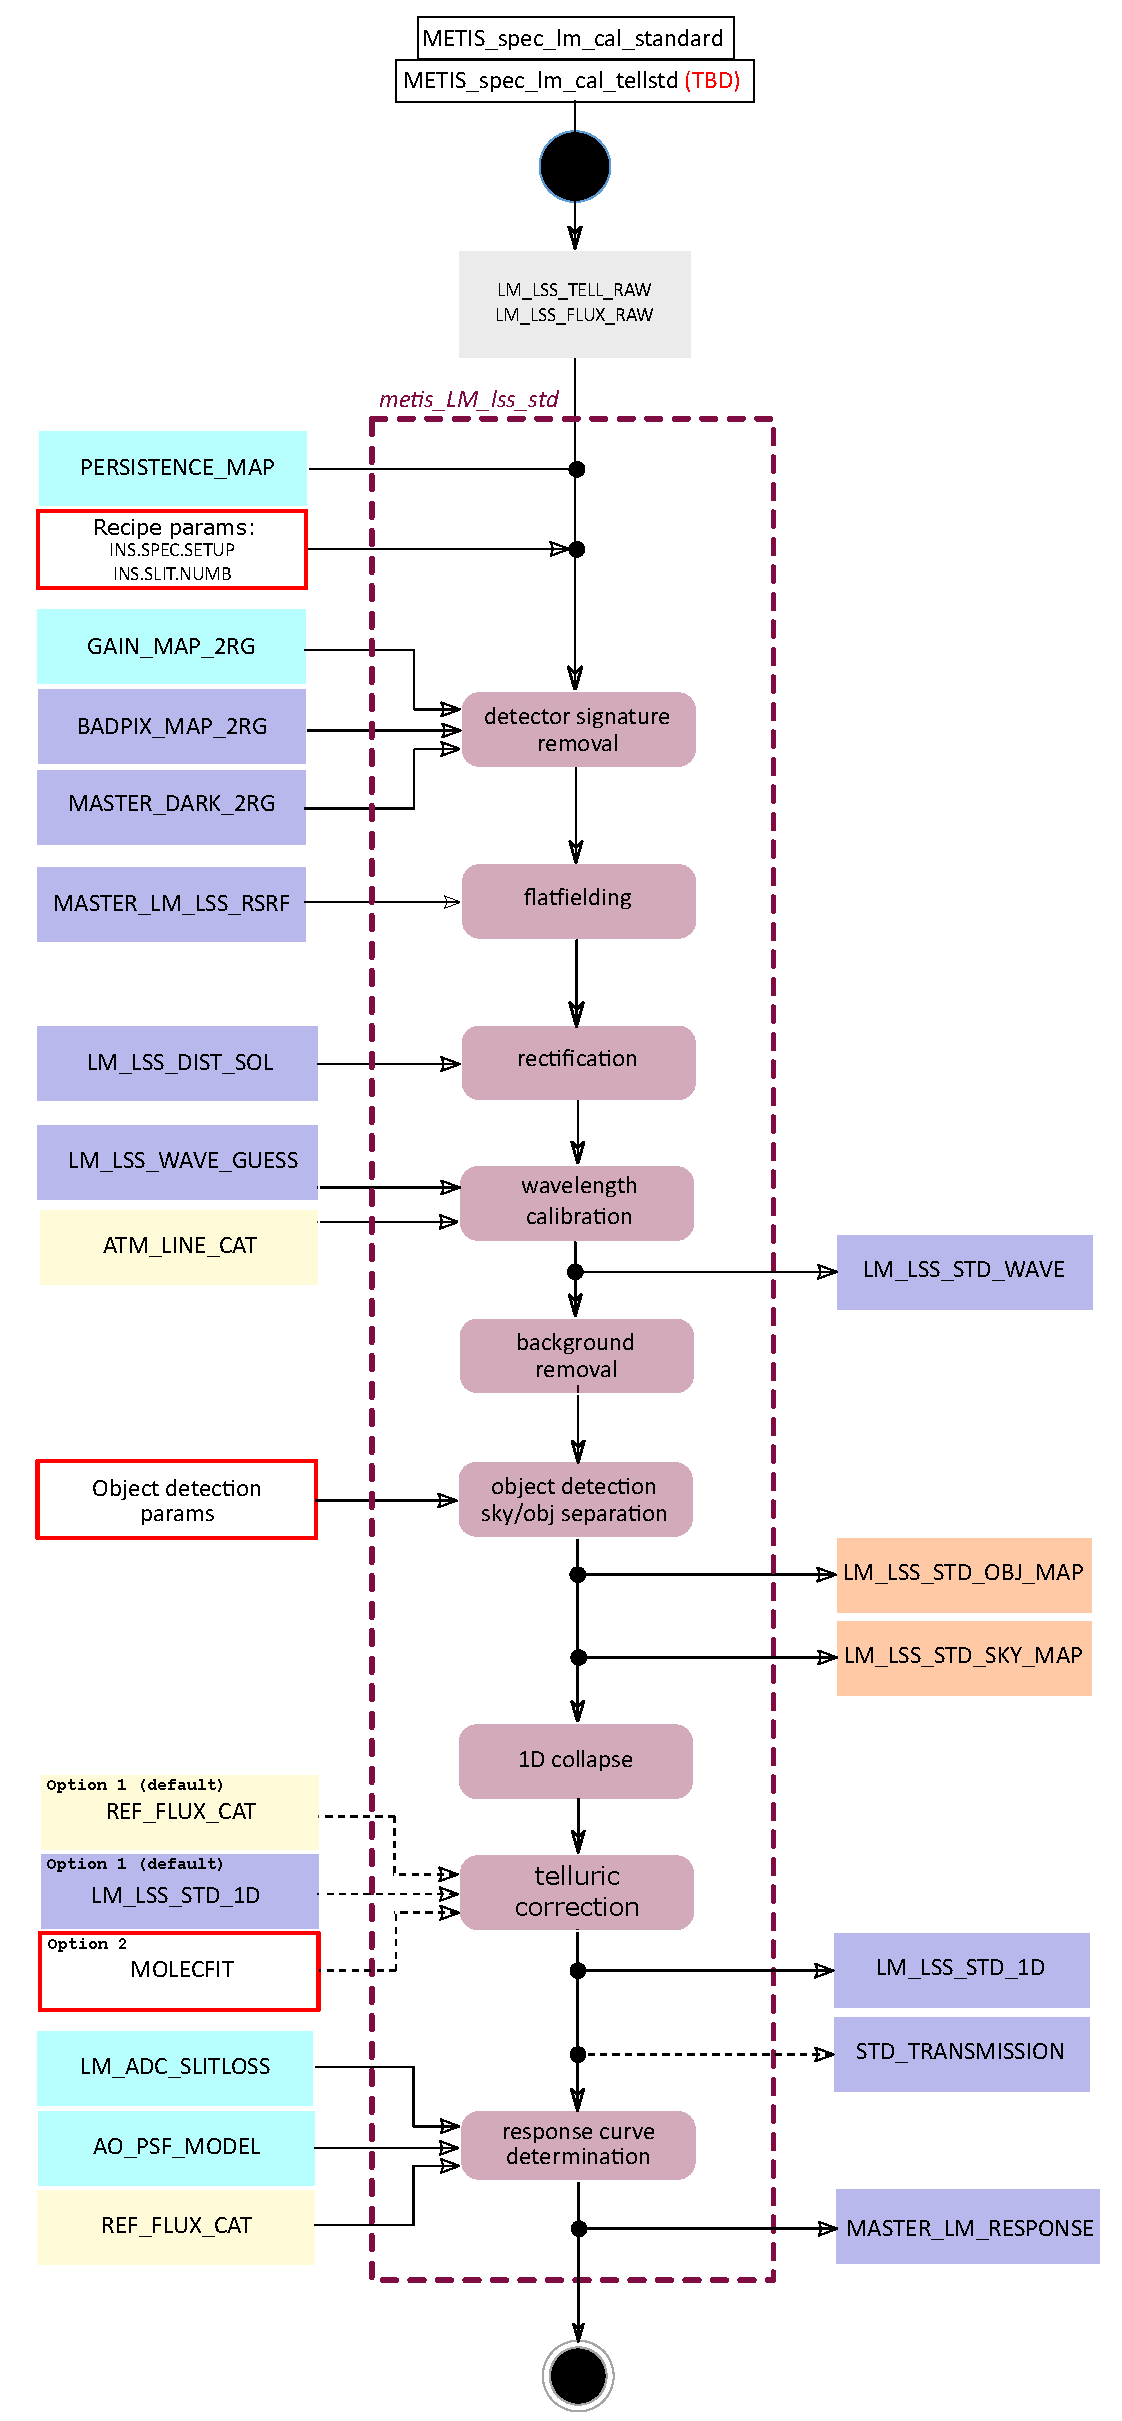
\includegraphics[width=0.4\textheight]{figures/metis_lm_lss_std_v0.82.pdf}
  \caption[Recipe: \REC{metis_LM_lss_std}]{\REC{metis_LM_lss_std} --
    Calibration recipe for processing standard stars for (combined) telluric and  spectro-photometric calibration.}
  \label{Fig:rec_lm_lss_flux1}
\end{figure}
%\begin{figure}[ht]
%  \centering
%  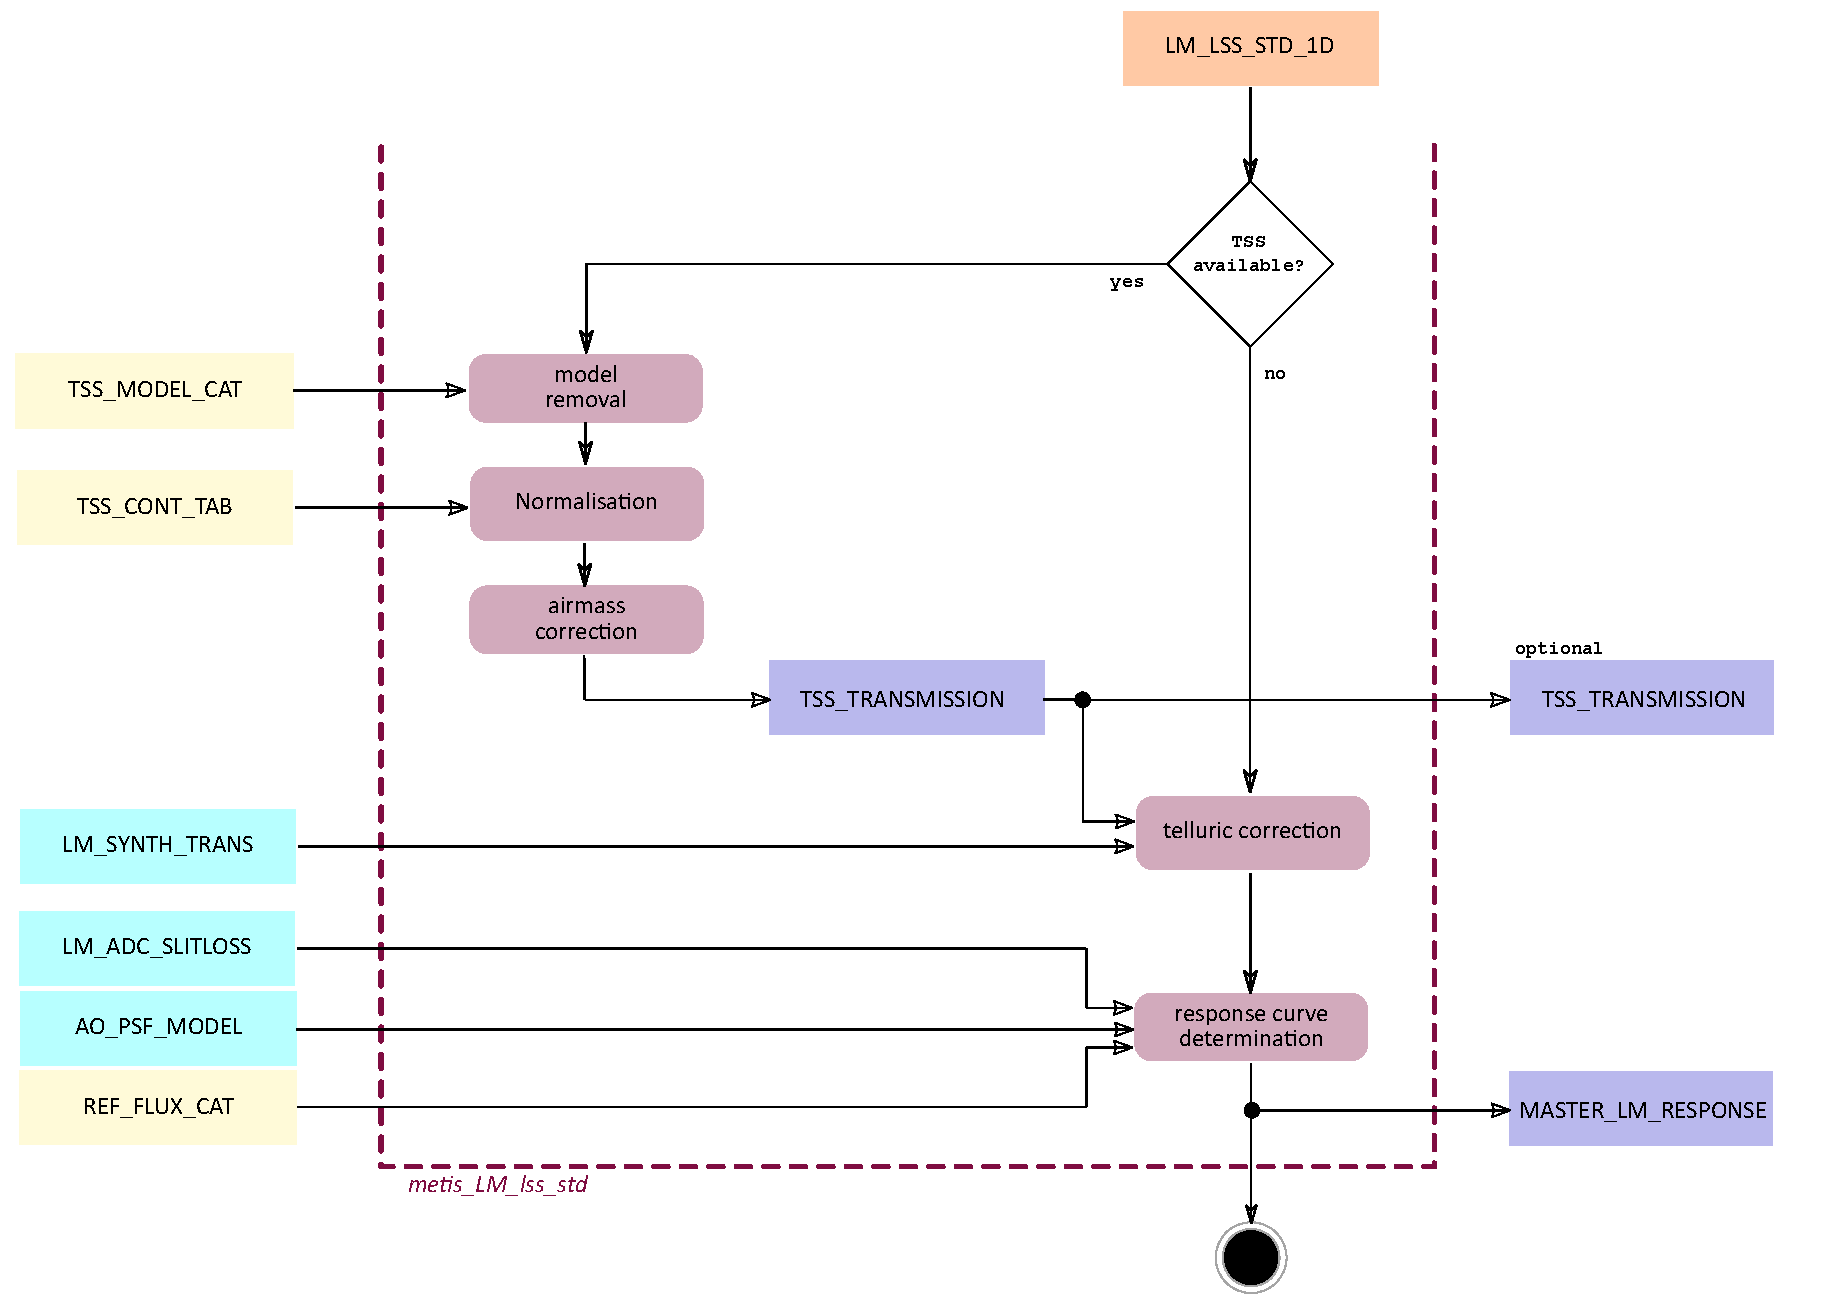
\includegraphics[width=0.6\textheight]{figures/metis_lm_lss_std_v0.8_part_2.pdf}
%  \caption[Recipe: \REC{metis_LM_lss_std}]{\REC{metis_LM_lss_std} --
%    Part 2 of the calibration recipe for processing spectrophotometric and telluric standard stars.}
%  \label{Fig:rec_lm_lss_flux2}
%\end{figure}
\clearpage
\begin{recipedef}
Name:		& \hyperref[rec:metis_lm_lss_std]{\REC{metis_LM_lss_std}} \\
Purpose:	& Flux calibration \\
Type:		& Calibration\\
Requirements: & METIS-6084, METIS-6074 \\
Templates:           & \TPL{METIS_spec_lm_cal_standard}\\
Input data: 	& \hyperref[dataitem:lm_lss_flux_raw]{\RAW{LM_LSS_FLUX_RAW}}\\
                & \hyperref[dataitem:persistence_map]{\EXTCALIB{PERSISTENCE_MAP}}  \\
                & \hyperref[dataitem:gain_map_lm]{\STATCALIB{GAIN_MAP_LM}}  \\
                & \hyperref[dataitem:badpix_map_lm]{\PROD{BADPIX_MAP_LM}}  \\
                & \hyperref[dataitem:master_dark_lm]{\PROD{MASTER_DARK_LM}}  \\
                & \hyperref[dataitem:master_lm_lss_rsrf]{\PROD{MASTER_LM_LSS_RSRF}} \\
                & \hyperref[dataitem:lm_lss_dist_sol]{\PROD{LM_LSS_DIST_SOL}} \\
                & \hyperref[dataitem:lm_lss_wave_guess]{\PROD{LM_LSS_WAVE_GUESS}} \\
                & \hyperref[dataitem:ao_psf_model]{\EXTCALIB{AO_PSF_MODEL}} \\
                & \hyperref[dataitem:atm_line_cat]{\EXTCALIB{ATM_LINE_CAT}} \\
%                & \hyperref[dataitem:tss_model_cat]{\STATCALIB{TSS_MODEL_CAT}}\\
%                & \hyperref[dataitem:tss_cont_tab]{\STATCALIB{TSS_CONT_TAB}}\\
                & \hyperref[dataitem:lm_adc_slitloss]{\STATCALIB{LM_ADC_SLITLOSS}}\\
                & \hyperref[dataitem:lm_synth_trans]{\STATCALIB{LM_SYNTH_TRANS}}\\
                & \hyperref[dataitem:ref_std_cat]{\STATCALIB{REF_STD_CAT}} \\
Parameters: 	& (TBD)\\
Algorithm:      & Application of master calibration files\\
                & Background removal\\
                & Determination and application of the distortion correction\\
                & Determination and application of the wavelength solution\\
                & Identifying/separatiing sky/object pixels\\
                & Removing sky lines: Creation and Subtraction of 2D sky\\
                & Collapsing 2D to 1D spectrum, (see Fig.\,\ref{Fig:rec_lm_lss_sci})\\
                & Determination and application of response curve\\
Output data:	& \hyperref[dataitem:lm_lss_std_obj_map]{\PROD{LM_LSS_STD_OBJ_MAP}}: Pixel map of object pixels\\
            	& \hyperref[dataitem:lm_lss_std_sky_map]{\PROD{LM_LSS_STD_SKY_MAP}}: Pixel map of sky pixels\\
              	& \hyperref[dataitem:lm_lss_std_1d]{\PROD{LM_LSS_STD_1D}}: coadded, wavelength calibrated, collapsed 1D spectrum\\
              	& \hyperref[dataitem:lm_lss_std_wave]{\PROD{LM_LSS_STD_WAVE}}: Wavelength solution derived from the \ac{STD} star (optional)\\
            	& \hyperref[dataitem:std_transmission]{\PROD{STD_TRANSMISSION}}: Transmission function derived by means of the \ac{STD} (optional)\\        
                & \hyperref[dataitem:master_lm_response]{\PROD{MASTER_LM_RESPONSE}}: response function \\
Expected accuracies: & 10\% over an atmospheric band (ESO Req. R-MET-107)\\
            & $<30$\% absolute line flux accuracy (R-MET-107)\\
            & $<5$\% absolute flux calibration (R-MET-82)\\
QC1 parameters: & \hyperref[qc:lmlssstdbackgdmean]{\QC{QC LM LSS STD BACKGD MEAN}}: Mean value of background\\
                & \hyperref[qc:lmlssstdbackgdmedian]{\QC{QC LM LSS STD BACKGD MEDIAN}}: Median value of background\\
                & \hyperref[qc:lmlssstdbackgdstdev]{\QC{QC LM LSS STD BACKGD STDEV}}: Standard deviation value of background\\
                & \hyperref[qc:lmlssstdsnr]{\QC{QC LM LSS STD SNR}}: Signal-to-noise ration of flux standard star spectrum\\
                & \hyperref[qc:lmlssstdsnrnoise]{\QC{QC LM LSS STD SNRNOISE}}: Noise level of flux standard star spectrum\\
                & \hyperref[qc:lmlssstdfwhm]{\QC{QC LM LSS STD FWHM}}: FWHM of flux standard spectrum\\
                & \hyperref[qc:lmlssfluxintrordravglevel]{\QC{QC LM LSS FLUX INTORDR LEVEL}}: Flux level of the interorder background\\
                & \hyperref[qc:lmlssfluxlevel]{\QC{QC LM LSS FLUX AVGLEVEL}}: Average level of the standard star flux \\
                & \hyperref[qc:lmlssfluxwavecaldevmean]{\QC{QC LM LSS FLUX WAVECAL DEVMEAN}}: Mean deviation from the
                  wavelength reference frame (TBDef)\\
                & \hyperref[qc:lmlssfluxwavecalfwhm]{\QC{QC LM LSS FLUX WAVECAL FWHM}}: Measured FWHM of lines\\
                & \hyperref[qc:lmlssfluxwavecalnident]{\QC{QC LM LSS FLUX WAVECAL NIDENT}}: Number of identified lines\\
                & \hyperref[qc:lmlssfluxwavecalnmatch]{\QC{QC LM LSS FLUX WAVECAL NMATCH}}: Number of lines matched between
                    catalogue and spectrum\\
                & \hyperref[qc:lmlssfluxwavecalpolydeg]{\QC{QC LM LSS FLUX WAVECAL POLYDEG}}: Degree of the polynomial\\
                & \hyperref[qc:lmlssfluxwavecalpolycoeffn]{\QC{QC LM LSS FLUX WAVECAL POLYCOEFF\<n\>}}: $n$-th coefficient of the polynomial\\
                & \hyperref[qc:lmlssfluxstdsnr]{\QC{QC LM LSS FLUX STDSNR}}: Signal-to-noise ration of flux standard star spectrum\\
                & \hyperref[qc:lmlssfluxsnrnoise]{\QC{QC LM LSS FLUX SNRNOISE}}: Noise level of flux standard star spectrum\\
                & \hyperref[qc:lmlssfluxfwhm]{\QC{QC LM LSS FLUX FWHM}}: FWHM of flux standard spectrum\\
                & \hyperref[qc:lmlssfluxpsfloss]{\QC{QC LM LSS FLUX PSFLOSS}}: Fraction of AO induced slit losses (TBdef)\\
                & more TBD
\end{recipedef}

\subsubsection{LM-LSS science reduction recipe \REC{metis_LM_lss_sci}:}\label{rec:metis_lm_lss_sci}
The science calibration recipe comprises the extraction of the object (i.e. separation of object/sky pixels), removing the sky lines, the application of the response curve previously defined, the 2D to 1D collapse and the co-addition. In contrast to the flux standard star reduction, the telluric correction on the science data is done in a dedicated recipe afterwards to achieve best quality for the correction.
\begin{figure}[ht]
  \centering
  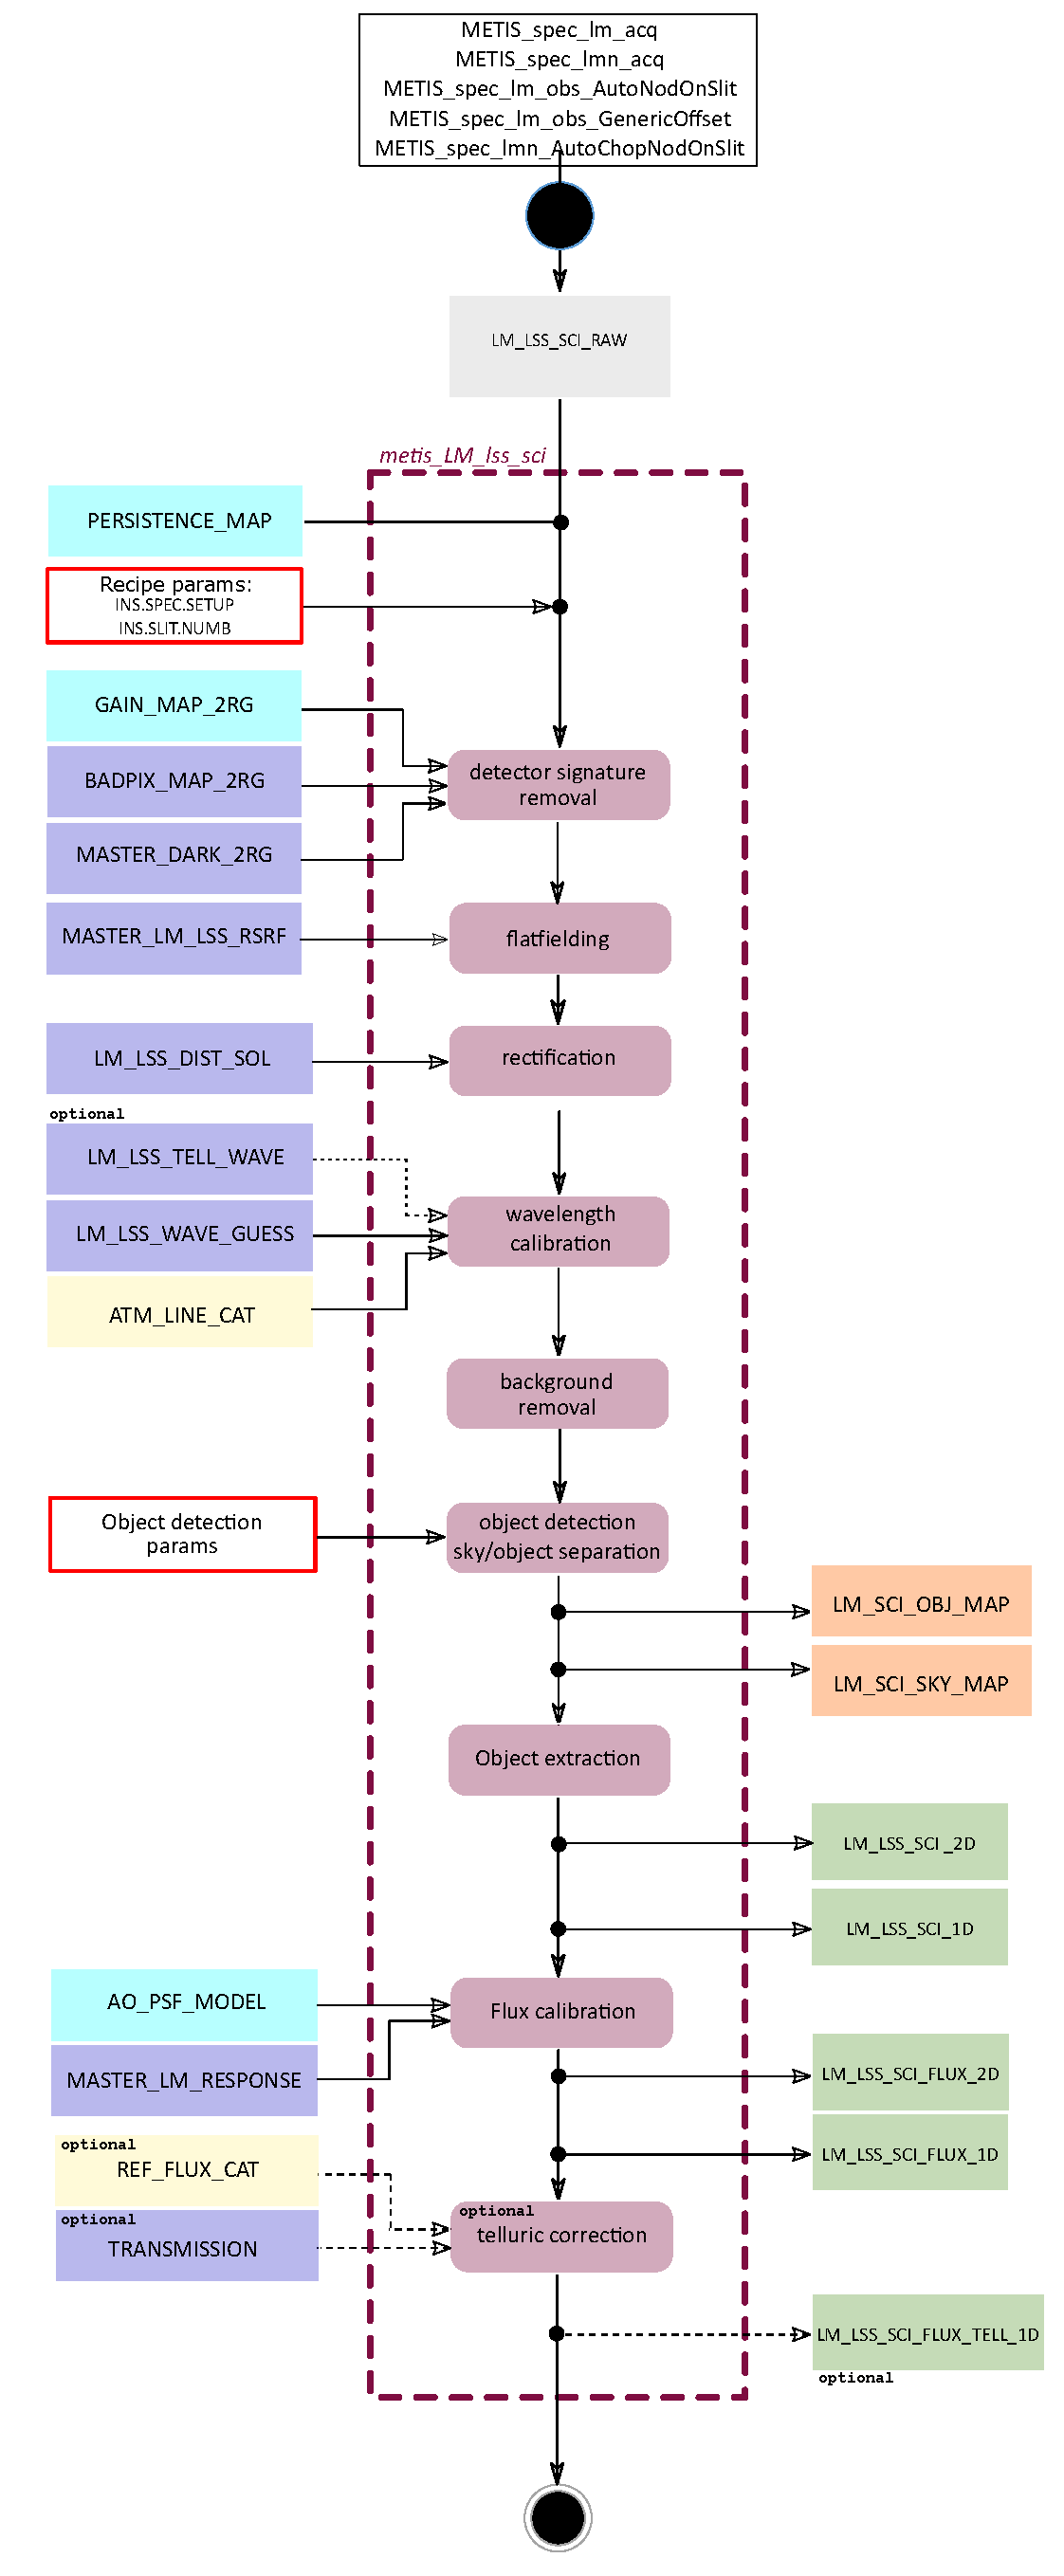
\includegraphics[width=0.37\textheight]{figures/metis_lm_lss_sci_v0.82.pdf}
  \caption[Recipe: \REC{metis_LM_lss_sci}]{\REC{metis_LM_lss_sci} --
    Science reduction recipe.}
  \label{Fig:rec_lm_lss_sci}
\end{figure}
\clearpage

\begin{recipedef}
Name:		& \hyperref[rec:metis_lm_lss_sci]{\REC{metis_LM_lss_sci}} \\
Purpose:    & Science data calibration\\
Type:		& Science reduction\\
Requirements: & METIS-6084 \\
Templates:           & \TPL{METIS_spec_lm_acq}, \\
                & \TPL{METIS_spec_lm_obs_AutoNodOnSlit}, \\
                & \TPL{METIS_spec_lm_obs_GenericOffset} \\
                & \TPL{METIS_spec_lm_cal_SlitAdc}\\
Input data: 	& \hyperref[dataitem:lm_lss_sci_raw]{\RAW{LM_LSS_SCI_RAW}}\\
                & \hyperref[dataitem:persistence_map]{\EXTCALIB{PERSISTENCE_MAP}}  \\
                & \hyperref[dataitem:gain_map_lm]{\STATCALIB{GAIN_MAP_LM}}  \\
                & \hyperref[dataitem:badpix_map_lm]{\PROD{BADPIX_MAP_LM}}  \\
                & \hyperref[dataitem:master_dark_lm]{\PROD{MASTER_DARK_LM}}  \\
                & \hyperref[dataitem:master_lm_lss_rsrf]{\PROD{MASTER_LM_LSS_RSRF}} \\
                & \hyperref[dataitem:lm_lss_dist_sol]{\PROD{LM_LSS_DIST_SOL}} \\
                & \hyperref[dataitem:lm_lss_wave_guess]{\PROD{LM_LSS_WAVE_GUESS}} \\
                & \hyperref[dataitem:atm_line_cat]{\EXTCALIB{ATM_LINE_CAT}} \\
                & \hyperref[dataitem:lm_adc_slitloss]{\STATCALIB{LM_ADC_SLITLOSS}}\\
            	& \hyperref[dataitem:std_transmission]{\PROD{STD_TRANSMISSION}} (optional)\\             
                %& \hyperref[dataitem:ao_psf_model]{\EXTCALIB{AO_PSF_MODEL}} \\
                %& \hyperref[dataitem:lsf_kernel]{\STATCALIB{LSF_KERNEL}}\\
                & \hyperref[dataitem:master_lm_response]{\PROD{MASTER_LM_RESPONSE}} \\
Parameters: 	& (TBD)\\
Algorithm:      & Application of the detector master calib files\\
                & wavelength calibration \\
                & Identifying/separatiing sky/object pixels\\
                & Removing sky lines: Creation and Subtraction of 2D sky\\
                & Coaddition of individual object spectra of one OB\\
                & Collapsing 2D to 1D spectrum, (see Fig.\,\ref{Fig:rec_lm_lss_sci})\\
                & Application of the response function (flux calibration) \\
Output data:	& \hyperref[dataitem:lm_lss_sci_obj_map]{\PROD{LM_LSS_SCI_OBJ_MAP}}: Pixel map of object pixels\\
            	& \hyperref[dataitem:lm_lss_sci_sky_map]{\PROD{LM_LSS_SCI_SKY_MAP}}: Pixel map of sky pixels\\
            	& \hyperref[dataitem:lm_lss_sci_2d]{\PROD{LM_LSS_SCI_2D}}: coadded, wavelength calibrated 2D spectrum\\
                & (\FITS{PRO_CATG}: \FITS{LM_LSS_2d_coadd_wavecal}) \\
                & \hyperref[dataitem:lm_lss_sci_1d]{\PROD{LM_LSS_SCI_1D}}: coadded, wavelength calibrated 1D spectrum\\
                & (\FITS{PRO_CATG}: \FITS{LM_LSS_1d_coadd_wavecal}) \\
                & \hyperref[dataitem:lm_lss_sci_flux_2d]{\PROD{LM_LSS_SCI_FLUX_2D}}: coadded, wavelength + flux calibrated 2D spectrum\\
                & (\FITS{PRO_CATG}: \FITS{LM_LSS_2d_coadd_wavecal}) \\
              	& \hyperref[dataitem:lm_lss_sci_flux_1d]{\PROD{LM_LSS_SCI_FLUX_1D}}: coadded, wavelength + flux 1D spectrum\\
                & (\FITS{PRO_CATG}: \FITS{LM_LSS_1d_coadd_wavecal}) \\
Expected accuracies: & (TBD)\\
QC1 parameters: & \hyperref[qc:lmlssscisnr]{\QC{QC LM LSS SCI SNR}}: Signal-to-noise ration of science spectrum\\
                & \hyperref[qc:lmlssscisnrnoise]{\QC{QC LM LSS SCI SNRNOISE}}: Noise level of science spectrum\\
                & \hyperref[qc:lmlssscifluxsnr]{\QC{QC LM LSS SCI FLUX SNR}}: Signal-to-noise ration of flux calibrated  science spectrum\\
                & \hyperref[qc:lmlssscifluxsnrnoise]{\QC{QC LM LSS SCI FLUX SNRNOISE}}: Noise level of flux calibrated science spectrum\\
                & \hyperref[qc:lmlsssciinterordrlevel]{\QC{QC LM LSS SCI INTORDR LEVEL}}: Flux level of the interorder background\\
                & \hyperref[qc:lmlsssciwavecaldevmean]{\QC{QC LM LSS SCI WAVECAL DEVMEAN}}: Mean deviation from the wavelength reference frame (TBDef)\\
                & \hyperref[qc:lmlsssciwavecalfwhm]{\QC{QC LM LSS SCI WAVECAL FWHM}}: Measured FWHM of lines\\
                & \hyperref[qc:lmlsssciwavecalnident]{\QC{QC LM LSS SCI WAVECAL NIDENT}}: Number of identified lines\\
                & \hyperref[qc:lmlsssciwavecalnmatch]{\QC{QC LM LSS SCI WAVECAL NMATCH}}: Number of lines matched between catalogue and spectrum\\
                & \hyperref[qc:lmlsssciwavecalpolydeg]{\QC{QC LM LSS SCI WAVECAL POLYDEG}}: Degree of the wavelength polynomial\\
                & \hyperref[qc:lmlsssciwavecalpolycoeffn]{\QC{QC LM LSS SCI WAVECAL POLYCOEFF\<n\>}}: $n$-th coefficient of the polynomial\\
                & more TBD\\
\end{recipedef}

\subsubsection{LM-LSS telluric correction recipe \REC{metis_LM_lss_mf_model}:}\label{rec:metis_lm_lss_mf_model}
The telluric correction will be done with the package \texttt{molecfit}\footnote{\url{https://www.eso.org/sci/software/pipelines/molecfit/molecfit-pipe-recipes.html}}. It is realised in three individual recipes, \hyperref[rec:metis_lm_lss_mf_model]{\REC{metis_LM_lss_mf_model}}, which calculates the best-fit model, \hyperref[rec:metis_lm_lss_mf_calctrans]{\REC{metis_LM_lss_mf_calctrans}}, which creates a synthetic transmission curve, and \hyperref[rec:metis_lm_lss_mf_correct]{\REC{metis_LM_lss_mf_correct}}, which performs the actual telluric correction by means of the synthetic transmission.

\begin{figure}[ht]
  \centering
  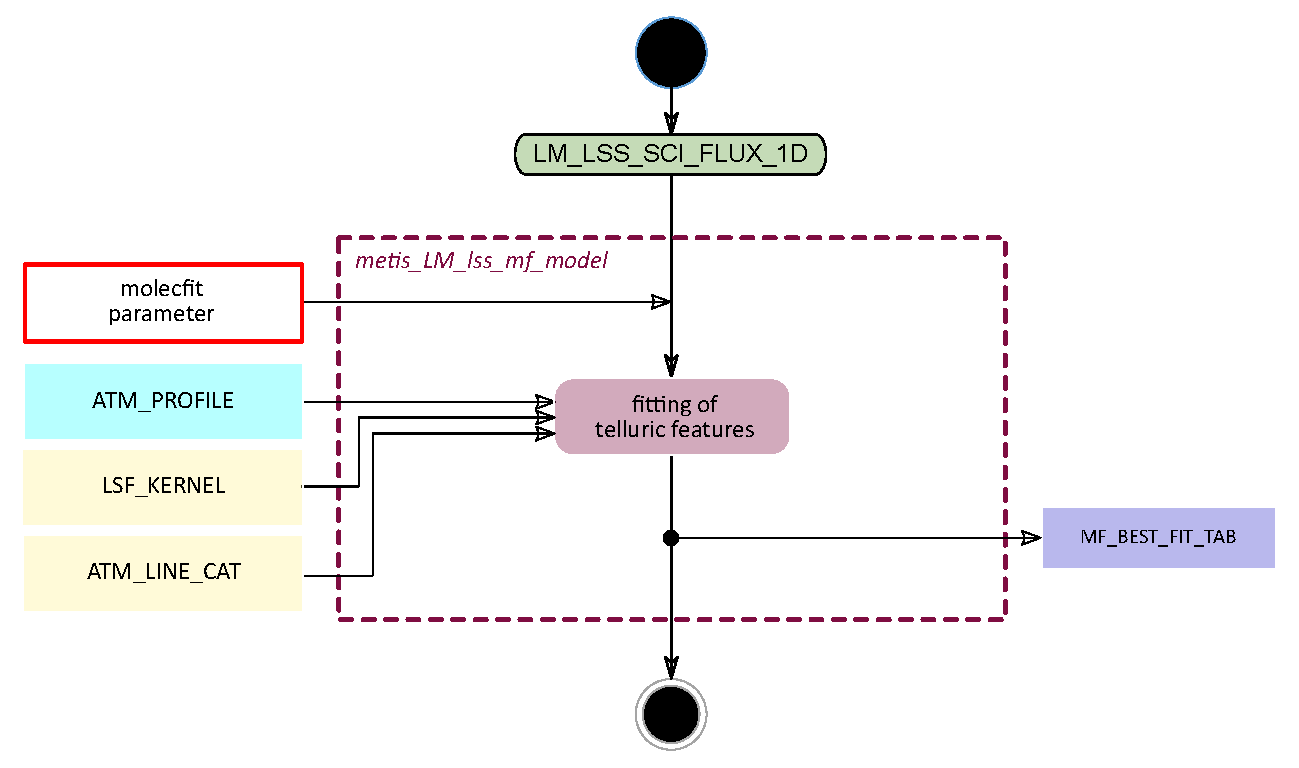
\includegraphics[width=0.5\textheight]{figures/metis_lm_lss_mf_model_v0.82.pdf}
  \caption[Recipe: \REC{metis_LM_lss_mf_model}]{\REC{metis_LM_lss_mf_model} --
    Recipe to achieve the best-fit for the calculation of the synthetic transmission curve for the telluric correction.}
  \label{Fig:rec_lm_lss_mf_model}
\end{figure}
\clearpage

\begin{recipedef}
Name:		& \hyperref[rec:metis_lm_lss_mf_model]{\REC{metis_LM_lss_mf_model}} \\
Purpose:	& Achieve the best fit for modelling the transmission curve to be applied as telluric correction \\
Type:		& Post-calibration\\
Requirements: & METIS-4051, METIS-6091 \\
Templates:           & None\\
Input data: 	& \hyperref[dataitem:lm_lss_sci_flux_1d]{\PROD{LM_LSS_SCI_FLUX_1D}}\\
                & \hyperref[dataitem:lsf_kernel]{\STATCALIB{LSF_KERNEL}} \\
                & \hyperref[dataitem:atm_profile]{\EXTCALIB{ATM_PROFILE}} \\
                & \hyperref[dataitem:atm_line_cat]{\EXTCALIB{ATM_LINE_CAT}} \\
Parameters: 	& \texttt{molecfit} parameters (c.f. \cite{molecfit})\\
Algorithm:      & Fit of telluric features visible in the science input spectrum\\
                & Determination of best-fit parameter set\\
Output data:	& \hyperref[dataitem:mf_best_fit_tab]{\PROD{MF_BEST_FIT_TAB}}: Table with best-fit parameters\\
Expected accuracies: & (TBD)\\
QC1 parameters: & cf. \cite{molecfit}\\
\end{recipedef}

\subsubsection{LM-LSS telluric correction recipe \REC{metis_LM_lss_mf_calctrans}:}\label{rec:metis_lm_lss_mf_calctrans}

\begin{figure}[ht]
  \centering
  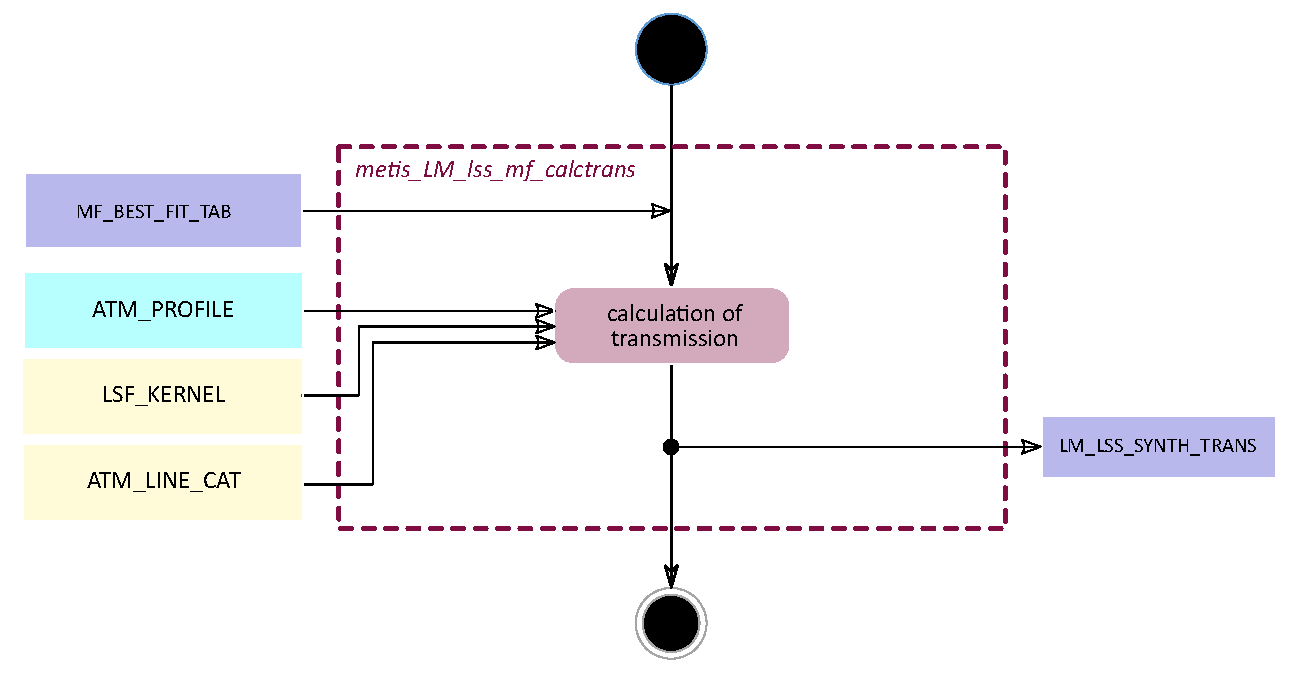
\includegraphics[width=0.5\textheight]{figures/metis_lm_lss_mf_calctrans_v0.82.pdf}
  \caption[Recipe: \REC{metis_LM_lss_mf_calctrans}]{\REC{metis_LM_lss_mf_calctrans} --
    Recipe to calculate the synthetic transmission to be applied as telluric correction.}
  \label{Fig:rec_lm_lss_mf_calctrans}
\end{figure}
\clearpage

\begin{recipedef}
Name:		& \hyperref[rec:metis_lm_lss_mf_calctrans]{\REC{metis_LM_lss_mf_calctrans}} \\
Purpose:	& Calculation of the synthetic transmission \\
Type:		& Post-calibration\\
Requirements: & METIS-4051, METIS-6091 \\
Templates:           & None\\
Input data: 	& \hyperref[dataitem:mf_best_fit_tab]{\PROD{MF_BEST_FIT_TAB}}: Table with best-fit parameters\\
                & \hyperref[dataitem:lsf_kernel]{\STATCALIB{LSF_KERNEL}} \\
                & \hyperref[dataitem:atm_profile]{\EXTCALIB{ATM_PROFILE}} \\
                & \hyperref[dataitem:atm_line_cat]{\EXTCALIB{ATM_LINE_CAT}} \\
Parameters: 	& \texttt{molecfit} parameters (c.f.  \cite{molecfit})\\
Algorithm:      & Calculate the entire transmission curve by means of the best-fit parameters\\
Output data:	& \hyperref[dataitem:lm_lss_synth_trans]{\PROD{LM_LSS_SYNTH_TRANS}}: synth. transmission\\
Expected accuracies: & (TBD)\\
QC1 parameters: & cf. \cite{molecfit}\\
\end{recipedef}

\subsubsection{LM-LSS telluric correction recipe \REC{metis_LM_lss_mf_correct}:}\label{rec:metis_lm_lss_mf_correct}

\begin{figure}[ht]
  \centering
  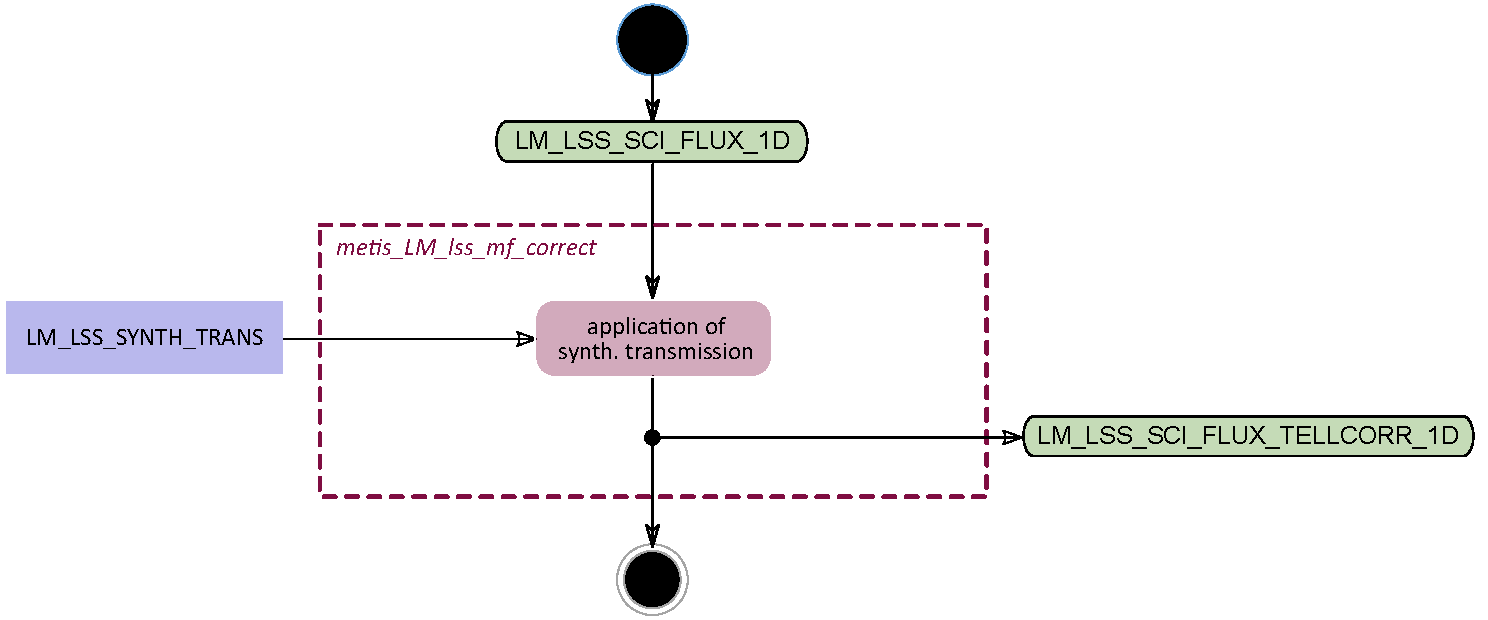
\includegraphics[width=0.5\textheight]{figures/metis_lm_lss_mf_correct_v0.82.pdf}
  \caption[Recipe: \REC{metis_LM_lss_mf_correct}]{\REC{metis_LM_lss_mf_correct} --
    Recipe to apply the telluric correction.}
  \label{Fig:rec_lm_lss_mf_correct}
\end{figure}
\clearpage

\begin{recipedef}
Name:		& \hyperref[rec:metis_lm_lss_mf_correct]{\REC{metis_LM_lss_mf_correct}} \\
Purpose:	& Apply the synthetic transmission to the science spectra \\
Type:		& Post-calibration\\
Requirements: & METIS-4051, METIS-6091 \\
Templates:           & None\\
Input data: 	& \hyperref[dataitem:lm_lss_sci_flux_1d]{\PROD{LM_LSS_SCI_FLUX_1D}}\\
                & \hyperref[dataitem:lm_lss_synth_trans]{\PROD{LM_LSS_SYNTH_TRANS}}\\
Parameters: 	& None\\
Algorithm:      & Apply telluric correction, i.e. divide the input science spectrum\\
                & by the synthetic transmission\\
Output data:	& \hyperref[dataitem:lm_lss_sci_flux_tellcorr_1d]{\PROD{LM_LSS_SCI_FLUX_TELLCORR_1D}}\\
Expected accuracies: & (TBD)\\
QC1 parameters: & cf. \cite{molecfit}\\
\end{recipedef}




% \input{06_4-Recipes_LSS_N}
% \input{06_5-Recipes_IFU}
% \input{06_6-Recipes_HCI}

\clearpage


% \subsection{Specifications and requirements}
% \label{Subsec:polarion}
% \input{01-Requirements}


\end{document}

%%
%% THE END
%%
%%%%%%%%%%%%%%%%%%%%%%%%%%%%%%%%%%%%%%%%%%%%%%%%%%%%%%%%%%%%%%%%%%%%%%%%%%%%%
